%                                     MMMMMMMMM                                         
%                                                                             
%  MMO    MM   MMMMMM  MMMMMMM   MM    MMMMMMMM   MMD   MM  MMMMMMM MMMMMMM   
%  MMM   MMM   MM        MM     ?MMM              MMM$  MM  MM         MM     
%  MMMM 7MMM   MM        MM     MM8M    MMMMMMM   MMMMD MM  MM         MM     
%  MM MMMMMM   MMMMMM    MM    MM  MM             MM MMDMM  MMMMMM     MM     
%  MM  MM MM   MM        MM    MMMMMM             MM  MMMM  MM         MM     
%  MM     MM   MMMMMM    MM   MM    MM            MM   MMM  MMMMMMM    MM
%
%
%            - META-NET Language Whitepaper | German paper -
%
% 
% ----------------------------------------------------------------------------

\documentclass[]{../../metanetpaper}

%!TEX TS-program = xelatex
\RequireXeTeX %Force XeTeX check

\usepackage{polyglossia}
\setotherlanguages{dutch,english}

\hyphenation{al-go-rit-mi-sche ana-ly-se an-der-zijds ant-woord ant-woor-den Ask-Now au-to-ma-tic au-to-ma-ti-se-ren A-xen-do au-teurs-on-der-steu-nings-sy-ste-men be-dien-den be-doe-ling be-drijfs-do-mei-nen  be-drijfs-le-ven be-drijfs-spe-ci-fie-ke be-drij-ven be-grij-pen be-kij-ken be-lang-rij-ke be-na-de-ring be-oor-de-len be-schik-baar-heid  be-schrij-ven be-ta-ling be-trek-ke-lij-ke be-voor-deeld bij-ko-men-de bij-na bui-ten-ge-slo-ten com-mu-ni-ca-tie-no-den com-ple-xi-teit com-pu-ters con-fe-ren-ties copy-right-schen-din-gen crowd-sour-cing daad-wer-ke-lijk des-am-bi-gu-e-ring di-a-kri-ti-sche dichtst-bij-zijnde dien-sten Di-gi-ta-le di-gi-ta-le do-cu-men-ten
do-mein-mo-del-le-ring do-mi-nan-te dy-na-mi-sche eind-ge-brui-kers-toe-pas-sin-gen e-lec-tro-ni-ca e-lek-tro-ni-ca ele-men-ten e-ner-zijds e-qui-va-lent erf-goed e-va-lu-a-tie fei-te-lij-ke fi-nan-cie-rings-toe-zeg-gin-gen Frank-rijk func-tio-na-li-teit ge-brui-kers-ac-cep-ta-tie ge-brui-kers-er-va-ring ge-brui-kers-vrien-de-lij-ke ge-meen-schap-pe-lijke ge-net-werk-te Ge-noot-schap  ge-or-ga-ni-seerd ge-pu-bli-ceerd ge-stan-daar-di-seerd ge-stuur-de ge-za-men-lij-ke gram-ma-ti-ca-le hier-on-der Hier-on-der hoe-veel-heid in-ge-ni-eurs-we-ten-schap-pen In-ter-net-do-mei-nen in-te-res-sant ken-nis-ma-na-ge-ment kern-roe-pas-sin-gen ko-nink-lij-ke Ko-nink-lij-ke kwa-li-teit le-vert Lu-xem-burg mak-ke-lij-ker me-de-werk-ers meer-ta-lig-heid  ME-TA-VI-SI-ON ME-TA-RE-SEARCH ME-TA-SHA-RE mo-del-le-ren moe-der-taal-spre-kers moei-lijk mo-ge-lijk-he-den na-tuur-lij-ke na-tuur-lijk-heid nau-we-lijks Ne-der-land Ne-der-lands Ne-der-land-se nog-al nood-za-ke-lij-ker nood-za-ke-lij-ker-wijs  on-der-zoeks-or-ga-ni-sa-ties on-der-steund on-der-steu-nen on-der-steu-nings-pro-gram-ma on-der-zoeks-or-ga-ni-sa-tie ont-bre-kend ont-wik-ke-laars ont-wik-keld ont-wik-kel-de ont-wik-ke-ling oor-spron-ke-lij-ke or-ga-ni-sa-ties ou-de-ren per-soon-lij-ke pho-nes pu-blieke re-le-van-te rij-zen se-man-ti-sche spe-ci-fie-ke spre-ker-on-af-han-ke-lij-ke spre-kers sta-tis-ti-sche stra-te-gi-sche strij-den sym-bo-li-sche taal-mo-del-len Taal-unie taal-tech-no-lo-gi-sche taal-ver-wer-king ta-bel-len tech-no-lo-gi-sche te-ge-lij-ker-tijd te-gen-woor-dig tekst-ana-ly-se teks-ten tekst-ver-wer-kers par-sing toe-pas-sin-gen toe-pas-sings-om-ge-ving toe-pas-sings-ge-bie-den toe-pas-sings-ka-der toe-pas-sings-ont-wik-ke-laars toe-wij-zings-over-een-komst     Toe-wij-zings-over-een-komst trans-pa-ran-ten uit-ge-voerd uit-vin-ding uit-zon-de-ring ver-an-de-rin-gen  ver-ba-zing-wek-kend ver-e-nigd ver-ge-lij-ken ver-ge-lij-king ver-te-gen-woor-di-ger ver-wer-ken ver-wer-king ver-wer-ven  ver-ze-ke-ren vir-tu-ele vi-sie-ont-wik-ke-lings-pro-ces Vlaan-de-ren voor-deel voor-uit-gang wer-kers werk-woord-con-struc-ties werk-woor-den woor-den woor-den-boek-af-dek-king werk-woor-denwoord-groe-pen woord-volg-or-de zaak-voe-ring}

\title{Het Nederlands in het Digitale Tijdperk --- The Dutch Language in the Digital Age}

\subtitle{White Paper Series --- Witboekserie}

\author{
Jan Odijk~ {\small Universiteit Utrecht} \\
Catia Cucchiarini~ {\small Nederlandse Taalunie}\\
Walter Daelemans~ {\small Universiteit Antwerpen}\\
Alice Dijkstra~ {\small NWO}\\
Jean-Pierre Martens~ {\small Universiteit Gent}\\
Jacomine Nortier~ {\small Universiteit Utrecht}\\
Peter Spyns~ {\small Nederlandse Taalunie}\\
Remco van Veenendaal~ {\small TST-centrale}
}

\editors{
  Georg Rehm, Hans Uszkoreit\\(XXX, \textcolor{grey1}{editors})
}

\begin{document}

% Mocktitle
\maketitle
\null
\pagestyle{empty} 

\centerline{META-NET -- office@meta-net.eu -- http://www.meta-net.eu}

\vfill

\begin{small}
  \selectlanguage{dutch}
De ontwikkeling van dit witboek is gefinancierd door het Zevende Kaderprogramma en het  ondersteuningsprogramma voor ICT-beleid van de Europese Commissie onder de contracten T4ME (Toewijzingsovereenkomst 249119), CESAR (Toewijzingsovereenkomst 271022), META-NET4U (Toewijzingsovereenkomst 270893) en META-NORD (Toewijzingsovereenkomst 270899).
\end{small}

\bigskip
\begin{small}
  \selectlanguage{english}
  The development of this white paper has been funded by the Seventh
  Framework Programme and the ICT Policy Support Programme of the
  European Commission under the contracts T4ME (Grant Agreement 249119),
  CESAR (Grant Agreement 271022), METANET4U (Grant Agreement 270893)
  and META-NORD (Grant Agreement 270899).
\end{small}

\clearpage

\pagenumbering{Roman} 
\setcounter{page}{5}
\pagestyle{scrheadings}

\cleardoublepage


% --------------------------------------------------------------------------
\bsection*{Voorwoord --- Preface}

\begin{Parallel}[c]{78mm}{78mm}
\ParallelLText{\selectlanguage{dutch}

Dit witboek maakt deel uit van een serie die kennis over taaltechnologie en het potentieel ervan bevordert. Het richt zich op onderwijsspecialisten, journalisten, politici, taalgemeenschappen en anderen.    De beschikbaarheid en het gebruik van taaltechnologie in Europa verschilt per taal. Daarom verschillen de acties die nodig zijn om ondersteuning van onderzoek en ontwikkeling van taaltechnologie te bevorderen eveneens per taal. De vereiste acties hangen af van veel factoren, zoals de complexiteit van een taal en de omvang van de taalgemeenschap.

META-NET, een `Network of Excellence' gefinancierd door de Europese Commissie, heeft een analyse gemaakt van de huidige taalbronnen en -technologie{\"e}n. Deze analyse richtte zich op de 23 offici{\"e}le Europese talen en op andere belangrijke nationale en regionale talen in Europa. De resultaten van deze analyse suggereren dat er veel significante lacunes zijn voor iedere taal. Een gedetailleerdere expertanalyse en beoordeling van de huidige situatie zal ertoe bijdragen de impact van additioneel onderzoek te maximaliseren en risico's te verminderen.

META-NET bestaat uit 54 onderzoekscentra in 33 landen (XXX: November 2011, XXX p.~\pageref{metanetmembers}) die werken met belanghebbenden uit commerci{\"e}le bedrijven, overheidsagentschappen, onderzoeksorganisaties, softwarebedrijven, technologieleveranciers en Europese universiteiten. Samen cre{\"e}ren zij een gemeenschappelijke technologievisie en ontwikkelen daarbij een strategische onderzoeksagenda die laat zien hoe taaltechnologische toepassingen lacunes in het onderzoek aan kunnen pakken tegen 2020.

XXX The authors of this document are grateful to the authors of the White Paper on German for permission to re-use selected language-independent materials from their document. 
}

\ParallelRText{\selectlanguage{english}
This white paper is part of a series that promotes knowledge about language technology and its potential. It addresses journalists, politicians, language communities, educators and others. 
The availability and use of language technology in Europe varies between languages. Consequently, the actions that are required to further support research and development of language technologies also differ. The required actions depend on many factors, such as the complexity of a given language and the size of its community.

META-NET, a Network of Excellence funded by the European Commission, has conducted an  analysis of current language resources and technologies in this white paper series (p.~\pageref{whitepaperseries}). The analysis focused on the 23 official European languages as well as other important national and regional languages in Europe. The results of this analysis suggest that there are tremendous deficits in technology support and significant research gaps for each language. The given detailed expert analysis and assessment of the current situation will help maximise the impact of additional research.

As of November 2011, META-NET consists of 54 research centres from 33 European countries (p.~\pageref{metanetmembers}). META-NET is working with stakeholders from economy (software companies, technology providers and users), government agencies, research organisations, non-governmental organisations, language communities and European universities. Together with these communities, META-NET is creating a common technology vision and strategic research agenda for multilingual Europe 2020.

The authors of this document are grateful to the authors of the White Paper on German for permission to re-use selected language-independent materials from their document. } 


\ParallelPar
\end{Parallel}

\cleardoublepage


% --------------------------------------------------------------------------
\bsection*{XXX --- Table of Contents}

\tableofcontents

\addtocontents{toc}{\protect\thispagestyle{empty}\protect}
\addtocontents{toc}{{\Large\textsf{\centerline{HET NEDERLANDS IN HET DIGITALE TIJDPERK}}\par}}

\cleardoublepage


% --------------------------------------------------------------------------
\setcounter{page}{1}
\pagenumbering{arabic} 
\pagestyle{scrheadings}


% Start of origin language part
% --------------------------------------------------------------------------
\ssection[Managementsamenvatting]{Managementsamenvatting}

\selectlanguage{dutch}

\begin{multicols}{2}

    In de laatste zestig jaar is Europa een aparte politieke en economische structuur geworden, maar op cultureel en taalkundig gebied is het nog zeer divers. Dit heeft als consequentie dat van het Portugees tot het Pools en van het Italiaans tot het Iers alledaagse communicatie en communicatie op het gebied van het bedrijfsleven en politiek onvermijdelijk tegen taalgrenzen aanloopt. De instituten van de Europese Unie besteden ongeveer een miljard euro per jaar om hun beleid van meertaligheid te behouden, d.w.z. aan het vertalen van teksten en het tolken bij gesproken communicatie. Maar hoeft dit wel zo'n last te zijn? Moderne taaltechnologie en taalkundig onderzoek kunnen een significante bijdrage leveren aan het slechten van deze taalkundige grenzen. Taaltechnologie zal, wanneer het gecombineerd wordt met intelligente toestellen en toepassingen, in de toekomst in staat zijn Europeanen te helpen op een eenvoudige manier met elkaar te praten en met elkaar zaken te doen zelfs als ze geen gemeenschappelijke taal spreken.
   
 \boxtext{Taaltechnologie bouwt bruggen \\ voor de toekomst van Europa }

    De Nederlandse economie heeft veel baat bij de XXX �{\'e}ngemaakte Europese markt. In 2010 besloeg handel binnen de EU meer dan 74\% van de Nederlandse export \cite{CBSStats}.  Maar taalgrenzen kunnen de bedrijvigheid tot stilstand brengen, vooral voor het MKB, dat niet de financi{\"e}le middelen heeft om de situatie te veranderen. Het enige (ondenkbare) alternatief voor dit meertalige Europa zou zijn dat wordt toegestaan dat {\'e}{\'e}n enkele taal een dominante positie inneemt en op termijn alle andere talen zou vervangen.

    Een klassieke manier om de taalgrenzen te overwinnen is het leren van vreemde talen. Maar zonder technologische ondersteuning is het leren beheersen van de 23 offici{\"e}le talen van de lidstaten van de Europese Unie en ongeveer 60 andere Europese talen een onoverkomelijk obstakel voor de burgers van Europa, zijn economie, het politieke debat en wetenschappelijke vooruitgang.

    De oplossing ligt in het bouwen van essenti{\"e}le technologie{\"e}n die nieuwe mogelijkheden cre{\"e}ren. Die zullen de Europese actoren enorme voordelen bieden, niet alleen in de gemeenschappelijke Europese markt maar ook in handelsrelaties met derde landen, vooral de opkomende economie{\"e}n. Om dit doel te bereiken en de culturele en taalkundige verscheidenheid van Europa te bewaren, moet er eerst een systematische analyse uitgevoerd worden van de taalkundige bijzonderheden van alle Europese talen en van de huidige toestand van de taaltechnologische ondersteuning voor die talen.

    \boxtext{Taaltechnologie als een sleutel voor de toekomst}

    De gereedschappen voor automatisch vertalen en het verwerken van spraak die momenteel beschikbaar zijn op de markt schieten nog te kort voor deze ambitieuze doelstelling. De dominante actoren in het veld zijn voornamelijk in de Verenigde Staten gebaseerde private commerci{\"e}le ondernemingen. Al in de late jaren zeventig van de vorige eeuw was Europa zich bewust van het grote belang van taaltechnologie als een aanjager van Europese eenheid, en begon het zijn eerste onderzoeksprojecten zoals EUROTRA te financieren. Tegelijkertijd werden nationale projecten opgezet die waardevolle resultaten hebben gegenereerd maar nooit geleid hebben tot een georkestreerde Europese actie. In scherp contrast tot deze selectieve financieringsacties, hebben andere meertalige maatschappijen zoals India (22 offici{\"e}le talen) en Zuid-Afrika (11 offici{\"e}le talen) recentelijk nationale langetermijnprogramma's opgezet voor taalonderzoek en taaltechnologische ontwikkeling.

    De overheersende actoren in taaltechnologie verlaten zich vandaag de dag op onnauwkeurige statistische benaderingen die geen gebruik maken van diepere taalkundige methoden en kennis. Zo worden zinnen bijvoorbeeld automatisch vertaald door een nieuwe zin te vergelijken met duizenden eerder door mensen vertaalde zinnen. De kwaliteit van de output hangt in hoge mate af van de hoeveelheid en de kwaliteit van het beschikbare corpus. Hoewel het automatisch vertalen van simpele zinnen in talen met voldoende beschikbaar tekstmateriaal nuttige resultaten kan bereiken, zijn zulke oppervlakkige statistische methodes gedoemd te falen voor talen met een veel kleinere hoeveelheid corpusmateriaal of in het geval van zinnen met complexe structuren.

    De Europese Unie heeft daarom besloten projecten te financieren zoals EuroMatrix en EuroMatrixPlus (sinds 2006) en iTranslate4 (sinds 2010) die fundamenteel en toegepast onderzoek uitvoeren en taalbronnen genereren om taaltechnologische oplossingen van hoge kwaliteit voor alle Europese talen neer te zetten. Het analyseren van diepere structurele eigenschappen van talen is de enige manier om verder te komen als we toepassingen willen bouwen die goed werken voor de hele reeks van Europese talen.

    Europees onderzoek op dit gebied heeft al een aantal successen geboekt. Zo gebruiken de vertaaldiensten van de Europese Unie nu de MOSES open source software voor automatisch vertalen, die grotendeels ontwikkeld is via Europese onderzoeksprojecten. De Nederlands-Vlaamse programma's CGN en STEVIN hebben een significante hoeveelheid basistaalbronnen beschikbaar gemaakt, onderzoek uitgevoerd en de markt voor taaltechnologie gestimuleerd. Daarmee is een eerste stap gezet om de positie van het Nederlands in de moderne communicatie- en informatiemaatschappij te verzekeren. Maar Europa had de neiging, in plaats van voort te bouwen op de onderzoeksresultaten, ge{\"\i}soleerde onderzoeksactiviteiten met beperkte impact op de markt na te jagen. De economische waarde  van zelfs de eerste inspanningen kan men zien in het aantal spin-offs. Een bedrijf zoals Trados, dat opgericht werd in 1984, werd in 2005 aan het in het Verenigd Koninkrijk gebaseerde SDL verkocht.

    \boxtext{Taaltechnologie draagt bij aan \\ de eenmaking van Europa}

    Afgaande op de tot nu toe verkregen inzichten ziet het ernaar uit dat de huidige zogenaamde `hybride' technologie die diepe analyses met statistische methodes combineert in staat zal zijn de kloof tussen alle Europese talen en daar voorbij te overbruggen. Zoals deze serie van witboeken laat zien, is er een dramatisch verschil tussen de staten van Europa in de mate waarin zij voorbereid zijn voor taaloplossingen en de toestand van het onderzoek. Hoewel het Nederlands een van de beter van taalbronnen voorziene EU-talen is, is er toch nog verder onderzoek nodig voordat echt effectieve taaltechnologische oplossingen klaar zijn voor alledaags gebruik. Tegelijkertijd zijn er goede vooruitzichten dat het Nederlands sprekende deel van Europa een leidende internationale rol kan spelen op dit belangrijke technologische gebied.

    Het langetermijndoel van META-NET is het introduceren van taaltechnologie van hoge kwaliteit voor alle talen om politieke en economische eenheid te bereiken door culturele verscheidenheid. De technologie zal ertoe bijdragen bestaande grenzen te slechten en bruggen te bouwen tussen de talen van Europa. Daarvoor moeten wel alle belanghebbenden --- in de politiek, het onderzoek, het bedrijfsleven, en de maatschappij --- hun inspanningen voor de toekomst verenigen.

    Deze serie van witboeken is een aanvulling op andere strategische acties ondernomen door META-NET (zie de appendix voor een overzicht). Actuele informatie zoals de huidige versie van het META-NET visiedocument \cite{MNVision}  of de Strategische OnderzoeksAgenda (Strategic Research Agenda, SRA) kunt u vinden op de META-NET website: \url{http://www.meta-net.eu}
\end{multicols}

\clearpage


% --------------------------------------------------------------------------
\ssection[Gevaar voor onze Talen en een Uitdaging voor Taaltechnologie]{Gevaar voor onze Talen en  een Uitdaging voor Taaltechnologie}

\begin{multicols}{2}

We zijn getuige van een digitale revolutie die een dramatisch effect heeft op de communicatie- en informatiemaatschappij. Recente ontwikkelingen in de digitale informatie- en communicatietechnologie worden soms vergeleken met de uitvinding van de boekdrukkunst. Wat kan deze analogie ons vertellen over de toekomst van de Europese informatiemaatschappij en onze talen in het bijzonder?

\boxtext{XXX De digitale revolutie lijkt de uitvinding \\ van de boekdrukkunst.}

 Na de uitvinding van de boekdrukkunst werden ware doorbraken in communicatie- en kennisuitwisseling verwezenlijkt door bijv. de vertaling van de Bijbel in de lokale taal. In de daarop volgende eeuwen werden culturele technieken ontwikkeld om beter om te gaan met taalverwerking en kennisuitwisseling:
    \begin{itemize}
      \item de orthografische en grammaticale standaardisatie van belangrijke talen maakte de snelle verspreiding van nieuwe wetenschappelijke en intellectuele idee{\"e}n mogelijk;
      \item de ontwikkeling van offici{\"e}le talen stelde burgers in staat om te communiceren binnen bepaalde (vaak politieke) grenzen;
 	  \item het onderwijs en de vertaling van talen maakte uitwisseling over talen heen mogelijk;
 	  \item de creatie van uitgevers- en bibliografische richtlijnen verzekerde de kwaliteit en beschikbaarheid van gedrukt materiaal;
 	  \item de creatie van verschillende media zoals kranten, radio, televisie, boeken, en andere formaten bedienden verschillende communicatienoden.
     \end{itemize}

     In de laatste twintig jaar heeft de informatietechnologie eraan bijgedragen veel processen te automatiseren en makkelijker te maken:
    \begin{itemize}
 	\item desktop publishing software heeft typen en zetten vervangen;
 	\item Microsoft PowerPoint heeft transparanten voor overheadprojectors vervangen;
 	\item e-mail verstuurt en ontvangt documenten sneller dan een fax-machine;
 	\item Skype biedt goedkope Internet telefoonoproepen aan en verzorgt virtuele ontmoetingen;
 	\item Audio- and videocoderingsformaten maken het makkelijk om multimedia-inhoud uit te wisselen;
 	\item zoekmachines leveren trefwoordgebaseerde toegang tot webpagina's;
 	\item online diensten zoals Google Translate produceren snelle, ruwe vertalingen;
 	\item platforms voor sociale media zoals Facebook, Twitter, and Google+ maken communicatie, samenwerking, en het delen van informatie makkelijker.
     \end{itemize}

     Hoewel zulke hulpmiddelen en applicaties nuttig zijn, zijn ze nog niet in staat om een duurzame meertalige Europese maatschappij voor iedereen te ondersteunen met vrij verkeer van informatie en goederen.



\subsection{Taalgrenzen staan de Europese Informatiemaatschappij in de Weg}
  
    We kunnen niet precies voorspellen hoe de toekomstige informatiemaatschappij eruit gaat zien. Maar het is zeer waarschijnlijk dat de revolutie in de communicatietechnologie mensen die verschillende talen spreken op nieuwe manieren bij elkaar zal brengen. Dat legt druk op individuen om nieuwe talen te leren en vooral op ontwikkelaars om nieuwe technologische toepassingen te maken om wederzijds begrip en toegang tot deelbare kennis te verzekeren. In een globale economische en informatieruimte interageren meer talen, sprekers en inhoud sneller met nieuwe mediatypes. De huidige populariteit van sociale media (Wikipedia, Facebook, Twitter, YouTube, and, recentelijk, Google+) is maar het topje van de ijsberg.

\boxtext{XXX In een globale economische en informatieruimte interageren meer talen, sprekers en inhoud.}

    We kunnen vandaag de dag in een paar seconden gigabytes tekst rond de wereld sturen voordat we ons realiseren dat de tekst in een taal is die we niet begrijpen. Volgens een recent rapport van de Europese commissie schaft 57\% van de Internetgebruikers in Europa goederen en diensten aan in andere talen dan hun moedertaal (Engels is de meest gebruikte vreemde taal, gevolgd door Frans, Duits en Spaans). 55\% van de gebruikers lezen inhoud in een vreemde taal terwijl slechts 35\% een andere taal gebruikt om e-mails te schrijven of om commentaren te plaatsen op het Web \cite{EC1}.   Een paar jaar geleden was het Engels waarschijnlijk de lingua franca van het Web --- de overgrote meerderheid van inhoud op het Web was in het Engels --- maar de situatie is nu drastisch veranderd. De hoeveelheid online inhoud in andere Europese talen (en talen uit Azi{\"e} en het Midden Oosten) is explosief toegenomen.

Het is verrassend dat deze overal aanwezige digitale tweedeling niet veel publieke aandacht gekregen heeft; maar het doet toch een prangende vraag rijzen: Welke Europese talen zullen gedijen in de genetwerkte informatie- en kennismaatschappij, en welke zijn gedoemd te verdwijnen?

\subsection{Onze Talen in Gevaar}

    Hoewel de drukpers ertoe bijdroeg de uitwisseling van informatie in Europa te vergroten, leidde het ook tot het verdwijnen van veel Europese talen. Regionale en minderheidstalen werden zelden gedrukt en talen zoals het Cornish en Dalmatisch werden beperkt tot mondelinge vormen van overdracht, wat dan weer hun gebruiksbereik beperkte. Zal het Internet hetzelfde schokeffect hebben op onze talen?

\boxtext{XXX De ongeveer 80 talen van Europa zijn een van onze  belangrijkste culturele bezittingen.}

    De ongeveer 80 talen van Europa zijn een van zijn rijkste en belangrijkste culturele bezittingen, en een vitaal onderdeel van Europa's unieke sociale model \cite{EC2}.  Hoewel talen zoals Engels en Spaans waarschijnlijk zullen overleven in de opkomende digitale marktplaats, zouden veel Europese talen irrelevant kunnen worden in een genetwerkte maatschappij. Dit zou Europa's globale status verzwakken, en ingaan tegen het strategische doel om gelijke deelname voor iedere Europese burger te verzekeren ongeacht taal. 


Volgens een UNESCO rapport over meertaligheid zijn talen een essentieel medium om fundamentele rechten uit te oefenen zoals politieke expressie, onderwijs en deelname aan de maatschappij \cite{Unesco1}.


\subsection{Taaltechnologie is een Essenti{\"e}le Ondersteunende Technologie}

    In het verleden richtten investeringsinspanningen op het gebied van taalbehoud zich op taalonderwijs en vertaling. Volgens een schatting bedroeg de Europese markt voor vertaling, tolken, softwarelokalisatie en websiteglobalisatie 8.4 miljard euro in 2008 en er wordt een groei verwacht van 10\% per jaar \cite{EC3}.  En toch dekt dit getal slechts een klein gedeelte af van de huidige en toekomstige noden voor communicatie tussen talen. De meest overtuigende oplossing om het taalgebruik in het Europa van morgen zowel in de breedte als in de diepte te verzekeren is het gebruik van de gepaste technologie, zoals we ook technologie gebruiken om onze transport-, energie- en handicapnoden op te lossen.

    Digitale taaltechnologie (die zich richt op alle vormen van geschreven tekst en gesproken uitingen) helpt mensen samen te werken, handel te drijven, kennis te delen en deel te nemen aan sociale en politieke debatten ongeacht taalbarri{\`e}res en computervaardigheden. De technologie functioneert vaak onzichtbaar in complexe softwaresystemen om ons te helpen:
    \begin{itemize}
 	\item informatie te vinden met een zoekmachine op het internet;
 	\item spelling en grammatica te controleren in een tekstverwerker;
 	\item productaanbevelingen in een online winkel te bekijken;
 	\item de verbale instructies te horen van een navigatiesysteem in auto's;
 	\item webpagina's te vertalen via een online dienst.
    \end{itemize}

    Taaltechnologie bestaat uit een aantal essenti{\"e}le toepassingen die processen mogelijk maken in een groter toepassingskader. Het doel van de META-NET taalwitboeken is om vast te stellen hoe matuur deze kerntechnologie{\"e}n zijn voor iedere Europese taal.

\boxtext{XXX Europa benötigt für alle Sprachen robuste und preiswerte Sprachtechnologie.}

Om onze positie aan de frontlinie van de globale innovatie te behouden heeft Europa taaltechnologie nodig die aangepast is aan alle Europese talen, die robuust en betaalbaar is, en nauw ge{\"\i}ntegreerd in belangrijke softwareomgevingen. Zonder taaltechnologie zullen we niet in staat zijn een werkelijk effectieve interactieve multimedia en meertalige gebruikerservaring te bereiken in de nabije toekomst.

\subsection{Mogelijkheden voor Taaltechnologie}

    Op het gebied van het drukken werd de technologische doorbraak gevormd door het snelle kopi{\"e}ren van een tekstbeeld (een pagina) met een daartoe uitgeruste drukpers. Mensen moesten het harde werk van het opzoeken, lezen, vertalen en samenvatten van kennis doen. We moesten wachten tot Edison om gesproken taal vast te kunnen leggen --- en ook die technologie maakte niet meer dan analoge kopie{\"e}n.

    Digitale taaltechnologie kan nu de processen van vertaling, productie van inhoud en kennismanagement voor alle Europese talen automatiseren. Het kan intu{\"\i}tieve taal- of spraakgebaseerde interfaces mogelijk maken voor huishoudelijke elektronica, machineparken, voertuigen, computers en robots. Praktische commerci{\"e}le en industri{\"e}le toepassingen zijn nog in de initi{\"e}le stadia van ontwikkeling, maar de resultaten van onderzoek en ontwikkeling cre{\"e}ren echte toegang tot nieuwe mogelijkheden. Zo is automatisch vertalen al redelijk accuraat in specifieke domeinen, en experimentele toepassingen bieden meertalige informatie- en kennismanagement evenals productie van inhoud in veel Europese talen.

    Zoals voor de meeste technologie{\"e}n geldt, zijn ook de eerste taaltoepassingen zoals stemgebaseerde gebruikersinterfaces en dialoogsystemen ontwikkeld voor zeer gespecialiseerde domeinen, en zij laten vaak beperkte performantie zien. Maar er zijn enorme marktmogelijkheden in de onderwijs- en entertainmentsectoren voor de integratie van taaltechnologie{\"e}n in `games', cultureelerfgoedsites, `edutainment' pakketten, bibliotheken, simulatieomgevingen en trainingprogramma's. Mobiele informatiediensten, software voor het computerondersteund leren van talen, eLearning-omgevingen, gereedschappen voor zelfevaluatie en software voor plagiaatdetectie zijn maar enkele van de toepassingsgebieden waar taaltechnologie een belangrijke rol kan spelen. De populariteit van socialemediatoepassingen zoals Twitter en Facebook suggereren additionele noden voor gesofisticeerde taaltechnologie{\"e}n die het plaatsen van berichten kunnen controleren, discussies kunnen samenvatten, trends in opinievorming kunnen suggereren, emotionele reacties kunnen detecteren, en schendingen van copyright kunnen identificeren of misbruik opsporen.

    Taaltechnologie biedt de Europese Unie een enorm potentieel. Het kan ertoe bijdragen de complexe kwestie van meertaligheid in Europa aan te pakken --- het feit dat verschillende talen op natuurlijke wijze naast elkaar bestaan in Europese bedrijven, organisaties en scholen. Maar burgers moeten kunnen communiceren over deze taalgrenzen heen dwars door de Europese Gemeenschappelijk Markt, en taaltechnologie kan helpen deze laatste barri{\`e}re te overwinnen en daarmee het vrije en open gebruik van individuele talen ondersteunen. 

\boxtext{XXX Sprachtechnologie hilft, die „Behinderung“ durch Sprachenvielfalt zu überwinden.} 

Als we nog verder in de toekomst kijken zal innovatieve Europese meertalige taaltechnologie een maatstaf bieden voor onze globale partners wanneer zij hun eigen meertalige gemeenschappen hiervan willen voorzien. Taaltechnologie kan gezien worden als een vorm van `ondersteunende technologie' die de `handicap' van taaldiversiteit helpt overwinnen en de taalgemeenschappen toegankelijker voor elkaar maakt.

  Tot slot is ook het gebruik van taaltechnologie voor reddingsoperaties in rampgebieden waar succesvol functioneren een kwestie van leven of dood kan zijn een actief onderzoeksgebied: Toekomstige intelligente robots met meertalig vermogen hebben het potentieel om levens te redden.

\subsection{Uitdagingen voor Taaltechnologie}

Hoewel taaltechnologie aanzienlijke vooruitgang geboekt heeft in de laatste paar jaar is het huidige tempo van de technologische vooruitgang en productinnovatie te langzaam. 

\boxtext{XXX Das Tempo des technologischen Fortschritts ist derzeit zu langsam.}


Veelgebruikte technologie{\"e}n zoals programma's voor spellings- en grammaticacontrole in tekstverwerkers zijn typisch eentalig, en zijn alleen beschikbaar voor een handjevol talen. Online diensten voor automatisch vertalen zijn nuttig om snel een redelijke benadering van de inhoud van een document te genereren maar zijn nog hoogst problematisch als het gaat om zeer accurate en volledige vertalingen. 

Door de complexiteit van natuurlijke taal is het modelleren van ons taalgebruik in software en het testen ervan in de praktijk een lange en kostbare zaak die duurzame financieringstoezeggingen vereist. Europa moet daarom zijn pioniersrol behouden in het aangaan van de technologische uitdagingen voor een meertalige taalgemeenschap door nieuwe methodes uit te vinden om de ontwikkeling voor het hele gebied te versnellen. Dit zou zowel computationele innovaties als technieken zoals crowdsourcing kunnen omvatten.

\subsection{Taalverwerving bij Mensen en Machines}

 Om te illustreren hoe computers met taal omgaan en waarom het moeilijk is ze te programmeren om taal te gebruiken bekijken we kort hoe mensen eerste en tweede talen verwerven, en daarna hoe taaltechnologiesystemen werken.

\boxtext{XXX Der Mensch eignet sich Sprachfertigkeiten durch das Lernen anhand von Beispielen sowie zugrunde liegender Sprachregeln an.}

 Mensen verwerven taalvaardigheden op twee verschillende manieren. Baby's verwerven een taal door te luisteren naar de interactie tussen de ouders, broers en zussen en andere familieleden. Vanaf een jaar of twee produceren kinderen hun eerste woorden en korte woordcombinaties. Dit is alleen mogelijk omdat mensen een genetisch bepaalde aanleg hebben om te imiteren en daarna te rationaliseren wat ze horen.

    Een tweede taal leren op latere leeftijd vereist meer inspanning, vooral omdat het kind niet ondergedompeld is in een taalgemeenschap van moedertaalsprekers. Op school worden vreemde talen meestal verworven door grammaticale structuur, vocabularium en spelling te leren door driloefeningen die taalkundige kennis beschrijven in termen van abstracte regels, tabellen en voorbeelden Een vreemde taal leren wordt moeilijker naarmate men ouder is.

    De twee hoofdtypes van taaltechnologische systemen `verwerven' taalvaardigheden op een vergelijkbare manier. Statistische (of `datagedreven') benaderingen verkrijgen taalkundige kennis uit gigantische collecties van concrete voorbeeldteksten. Hoewel het volstaat om tekst van een enkele taal te gebruiken om bijv. een spellingchecker te ontwikkelen, moeten parallelle teksten in twee (of meer) talen beschikbaar zijn om een automatisch vertaalsysteem te ontwikkelen. Een `machine-learning' algoritme `leert' dan patronen voor de vertaling van woorden, korte frases en volledige zinnen.

    Deze statistische benadering kan miljoenen zinnen vereisen en de kwaliteit van de technologie neemt toe naarmate er meer tekst geanalyseerd wordt. Dit is een van de redenen waarom leveranciers van zoekmachinediensten zo graag zoveel mogelijk geschreven materiaal verzamelen. Spellingscorrectie in tekstverwerkers, en diensten zoals Google Search en Google Translate zijn allemaal gebaseerd op statistische benaderingen. Het grote voordeel van statistiek is dat de machine snel leert in continue series van trainingscycli hoewel de kwaliteit enorm kan verschillen.

    De tweede benadering van taaltechnologie en automatisch vertalen in het bijzonder bestaat uit het bouwen van regelgebaseerde systemen. Experts op het gebied van taalkunde, computationele taalkunde en informatica moeten eerst grammaticale analyses (vertaalregels) inbrengen en vocabulariumlijsten (lexicons) samenstellen. Dit is zeer tijds- en arbeidsintensief. Enkele van de regelgebaseerde automatische vertaalsystemen zijn al meer dan twintig jaar onder constante ontwikkeling. Het grote voordeel van regelgebaseerde systemen zit 'm in de gedetailleerde controle die experts hebben over de taalverwerking. Dat maakt het mogelijk om systematisch fouten in de software te corrigeren en gedetailleerde feedback te geven aan de gebruiker, vooral wanneer regelgebaseerde systemen gebruikt worden voor het leren van taal. Maar door de hoge kosten van dit werk is regelgebaseerde technologie tot nu toe alleen ontwikkeld voor de belangrijkste talen.

    Aangezien de sterktes en zwaktes van statistische en regelgebaseerde systemen complementair neigen te zijn, richt het huidige onderzoek zich op hybride benaderingen die de twee methodologie{\"e}n combineert. Tot nu toe zijn die benaderingen echter minder succesvol geweest in industri{\"e}le toepassingen dan in het onderzoekslaboratorium.

    Zoals we gezien hebben in dit hoofdstuk maken veel wijdverbreide toepassingen in de moderne informatiemaatschappij intensief gebruik van taaltechnologie. Vanwege de meertaligheid van de gemeenschap geldt dat in het bijzonder voor de Europese economische en informatieruimte. Hoewel taaltechnologie enorme vooruitgang geboekt heeft in de laatste paar jaar, ligt er nog een enorm potentieel om de kwaliteit van taaltechnologiesystemen te verbeteren. In de volgende secties zullen we de rol van het Nederlands in de informatiemaatschappij beschrijven en de huidige toestand van taaltechnologie voor het Nederlands evalueren.
 
\end{multicols}

\clearpage


% --------------------------------------------------------------------------
\ssection[Het Nederlands in de Europese Informatiemaatschappij]{Het Nederlands in de Europese Informatiemaatschappij}

\begin{multicols}{2}

\subsection{Algemene Feiten}

Met ongeveer 23 miljoen moedertaalsprekers is het Nederlands de achtste meest gesproken taal in de EU. Het is de algemeen gebruikte taal in Nederland en het Vlaamse deel (Vlaanderen) van Belgi{\"e} en een van de offici{\"e}le talen in Suriname, Aruba, Cura{\c{c}}ao en Sint-Maarten, waar het door delen van de bevolking wordt gebruikt. Het wordt ook gesproken in de EU in Frankrijk en Duitsland, en buiten de EU in Brazili{\"e}, Canada, Indonesi{\"e} (Java en Bali), Zuid-Afrika, en de Verenigde Staten. De offici{\"e}le Nederlandse naam voor de taal is Nederlands, hoewel Nederlands zoals gesproken in Vlaanderen gewoonlijk Vlaams genoemd wordt.

    Dit witboek richt zich op de toestand van het Nederlands en taal-technologie ervoor in Nederland en Vlaanderen, die we gezamen-lijk zullen aanduiden met de term `de Lage Landen'.

    In Nederland is het Nederlands de gemeenschappelijke geschreven en gesproken taal en de moedertaal van de overgrote meerderheid van de bevolking. Nederland heeft een officieel erkende minderheidstaal, het Fries, gesproken in de provincie Friesland. Er zijn verschillende immigrantentalen. Er zijn geen betrouwbare gegevens over de aantallen sprekers van immigrantentalen bekend. Maar het Centraal Bureau voor de Statistiek \cite{CBS} levert wel cijfers voor immigranten per etniciteit ($\neq$nationaliteit). Voor etniciteiten van buiten Nederland zijn er ongeveer 1.5 miljoen van westerse oorsprong, en voor niet-westerse herkomst zijn de cijfers: Marokko (Rif Berber, geschat op 75\%, en (Marokkaans) Arabisch, geschat op 25\%) 350k personen, Nederlandse Antillen en Aruba (Papiamento) 138k personen, Suriname (Nederlands, Sranan, Guyaans Creools Engels, Hindustani, Javaans) 342k personen, Turkije (Turks) 383k personen, en andere niet-westerse landen (verschillende talen) 644k personen.

    In Belgi{\"e} is het Nederlands bij wet de taal van Vlaanderen, en een van de twee talen (naast Frans) van de regio Brussel. Belgi{\"e} heeft ook een Frans sprekende regio en een Duits sprekende regio.

    Het Nederlands heeft een vari{\"e}teit aan dialecten, waaronder (in Nederland) Achterhoeks, Drents, Gronings, Limburgs, Sallands, Stellingwerfs, Twents, Veluws en Zeeuws, en in Vlaanderen West-Vlaams, Antwerps, Oost-Vlaams, Brabants en Limburgs. De orthografie is gestandaardiseerd maar er zijn recentelijk (1996 and 2006) wat veranderingen in de standaard doorgevoerd. De standaard is verplicht in onderwijs en overheidspublicaties. Enkele van de recent voorgestelde wijzigingen hebben geleid tot verschillende interpretaties van de standaard door verschillende uitgevers, wat heeft geresulteerd in kleine spellingsverschillen (bijv. \emph{het Groene Boekje} \cite{GroeneBoekje}: \emph{actievoeren} v. \emph{Van Dale}: \emph{actie voeren}), en enkele spellingsveranderingen werden niet geaccepteerd door alle uitgevers \cite{Wittespellers} , die daarom enkele woorden anders spellen (vooral met betrekking tot de zogenaamde \emph{tussen-n} in samenstellingen), in overeenstemming met het zogenaamde \emph{Witte Boekje} \cite{Wittespelling}.  De Nederlandse orthografie kan behoorlijk moeilijk zijn voor bepaalde woorden en constructies, zelfs zo moeilijk dat ieder jaar het zogenaamde \emph{Groot Dictee} \cite{Grootdictee} wordt georganiseerd door Nederland en Vlaanderen en uitgezonden op de nationale TV. Het \emph{Groot Dictee} is zo moeilijk dat iedereen die minder dan 30 fouten in ongeveer 8 zinnen maakt beschouwd kan worden als een excellent speller! Over het algemeen delen de Nederlandse dialecten in Nederland dezelfde kerngrammatica, hoewel sommige dialecten verschillen vertonen in bepaalde syntactische constructies. Er is een behoorlijk aantal lexicale verschillen tussen dialecten, en vooral tussen het Nederlands zoals gesproken in Nederland en het Nederlands zoals gesproken in Vlaanderen, bijv. het woord \emph{ajuin} wordt gebruikt in Vlaanderen in plaats van het Standaardnederlands \emph{ui}. Er zijn ook heel wat woorden die hetzelfde zijn in Vlaanderen en Nederland maar een andere betekenis hebben, bijv. \emph{middag} in Nederland betekent de periode van een dag van 14:00-17:00 uur, terwijl het in Vlaanderen de periode van de dag van 12:00-14:00 uur betekent. Het Vlaams gebruikt ook veel woorden die hun herkomst hebben in het Frans, bijv. termen voor auto-onderdelen, waar het Nederlands in Nederland eerder Engelse of op het Engels ge{\"\i}nspireerde woorden gebruikt. Dit heeft soms ook gevolgen voor de uitspraak, bijv. de woorden \emph{flat} en \emph{tram} worden zowel in Nederland als in Vlaanderen gebruikt, ze zijn ontleend aan het Engels, maar in Vlaanderen verliep de ontlening via het Frans, zodat deze woorden in Vlaanderen uitgesproken worden als fl[A]t en tr[A]m terwijl ze in het Nederlands uitgesproken worden als fl[E]t en tr[E]m.

\subsection{Eigenaardigheden van het Nederlands}

Het Nederlands vertoont enkele specifieke karakteristieken, die bijdragen aan de rijkdom van de taal door het sprekers mogelijk te maken idee{\"e}n tot uitdrukking te brengen op een groot aantal ver-schillende manieren. Een zo'n karakteristiek is dat het vrij gebruikelijk is om niet-onderwerpen vooraan in de zin te zetten (veel gebruikelijker dan in het Engels). Neem bijv. de Engelse zin \textit{The woman was going to the store every day.} In het Engels zijn er maar beperkte mogelijkheden om een andere woordvolgorde te gebruiken, maar in het Nederlandse equivalent kan bijna iedere woordgroep vooraan in de zin staan:

\begin{itemize}
\item De vrouw ging elke dag naar de winkel
\item    Elke dag ging de vrouw naar de winkel
\item    Naar de winkel ging de vrouw elke dag
\end{itemize}

\boxtext{XXX Bestimmte linguistische Merkmale des Deutschen stellen für Computer eine Herausforderung dar.}


    De woordvolgorde in het Nederlands is dan ook veel vrijer dan in het Engels (maar niet zo vrij als in het Duits).


    Het Nederlands heeft een vrij productief verschijnsel van woordvorming door nieuwe samenstellingen te maken, hoewel het gebruik en de productiviteit niet zo extreem zijn als in het Duits. Desondanks komen nieuwgevormde samenstellingen frequent voor en zij zijn moeilijk te verwerken voor taaltechnologie.

    Een andere karakteristiek van het Nederlands die automatische verwerking moeilijk maakt wordt gevormd door scheidbare werkwoordsprefixen die op kunnen treden op plaatsen in de zin ver weg van het werkwoord waar ze bij horen in geneste (`tang') constructies zoals:\\

\begin{itemize}
\item Hij \textbf{stelde} zich na mij een drankje aangeboden te hebben en wij in gesprek geraakt waren aan ons \textbf{voor}.
\end{itemize}

    De betekenis van een werkwoord dat een dergelijk scheidbaar prefix zoals \emph{voor}, \emph{in}, of \emph{uit} bevat kan zeer vaak niet afgeleid worden van de betekenis van het basiswerkwoord en de betekenis van het prefix. Het werkwoord \emph{stellen} (betekenis: `zetten, plaatsen') is bijvoorbeeld bevat in \emph{voorstellen} (betekenis: `inbeelden', `introduceren', etc.), \emph{instellen} (betekenis o.a. `afregelen')), \emph{uitstellen} (betekenis `opschorten') en in vele andere werkwoorden.

    Een andere eigenaardigheid die de automatische verwerking van het Nederlands compliceert is het verschijnsel van de zogenaamde R-pronomina zoals \emph{er, waar, daar}. Deze voornaamwoorden staan vaak verwijderd van het voorzetsel waar ze bij horen

\begin{itemize}
\item Hij keek daar gisteren naar.
\end{itemize}

    waar \textit{daar} en \textit{naar} van elkaar gescheiden worden door het bijwoord \textit{gisteren}. Verder kan een enkel voorkomen van het voornaamwoord \emph{er} meerdere functies tegelijkertijd vervullen, bijv. in

\begin{itemize}
\item Dachten er twee over na?
\end{itemize}

    waar \emph{er} tegelijkertijd bij het voorzetsel \emph{over} en bij het telwoord \emph{twee} hoort.


\subsection{Recente Ont\-wikke\-lin\-gen}

    Vanaf de jaren vijftig van de vorige eeuw begonnen Amerikaanse TV-series de Nederlandse markt te veroveren. Vreemde films en series worden over het algemeen uitgezonden in de originele taal en ondertiteld. De sterke aanwezigheid van de Amerikaanse manier van leven in de media heeft de Nederlandse taal en cultuur be{\"\i}nvloed. Dankzij de voortdurende triomf van de Engelse muziek sinds de jaren zestig (bijv. Elvis Presley, de Beatles), zijn generaties van jonge mensen opgegroeid in een omgeving waar het Engels natuurlijk was. Het Engels werd de `coole/hippe' taal en heeft die status tot op de dag van vandaag behouden.

    De voortdurende populariteit komt tot uitdrukking in het feit dat tegenwoordig leenwoorden vaak hun oorsprong hebben in het Engels. Volgens een schatting door \cite{VanderSijs:2005}, bestaat 30\% van het Nederlandse vocabularium uit leenwoorden, en vele ervan komen uit het Engels. In de meeste gevallen vullen deze woorden een lacune op, d.w.z. ze verrijken het Nederlands eerder dan er een bedreiging voor te vormen, hoewel sommige leenwoorden beschouwd worden als anglicismen, d.w.z. barbarismen uit het Engels waar geschikte Nederlandse equivalenten voor bestaan die bij voorkeur gebruikt zouden moeten worden.

    Leenwoorden uit het Engels domineren in het bedrijfsleven, de wetenschap, bepaalde technische domeinen en op het internet. Er kan ook een sterke tendens om Engels teveel te gebruiken waargenomen worden in productreclames.

    Deze ontwikkelingen laten zien hoe belangrijk het is mensen bewust te maken van een ontwikkeling die het risico inhoudt dat een deel van de bevolking buitengesloten wordt van deelname in de informatiemaatschappij, namelijk degenen die niet vertrouwd zijn met het Engels. Dit was ook een van de redenen om het Nederlands-Vlaamse taal- en spraaktechnologische programma STEVIN \cite{STEVIN}, dat beoogde de positie van het Nederlands in de moderne informatiemaatschappij te consolideren, op te starten.

\subsection{Taalcultivatie in de Lage Landen}

   Het Nederlands wordt vertegenwoordigd door verschillende publiek gefinancierde organisaties en taallichamen.

   Er is een intergouvernementele organisatie voor taalbeleid, de Nederlandse Taalunie \cite{NTU}, waarin Nederland, Vlaanderen en Suriname samenwerken op het gebied van de Nederlandse taal. Het beleid van de Taalunie wordt vastgesteld door het Comit{\'e} van Ministers, een commissie met de Nederlandse en Vlaamse ministers voor onderwijs en cultuur en een vertegenwoordiger van Suriname als leden. De Taalunie werkt ook samen met de Cara{\"\i}bische eilanden die het Nederlands als een offici{\"e}le taal hebben.

   Het beleid van de Nederlandse Taalunie betreft de Nederlandse taal zelf, het Nederlands in digitale toepassingen, het onderwijs van de Nederlandse taal, literatuur, het bevorderen van leesvaardigheden, de positie van het Nederlands in Europa en de wereld, en tot slot de niet geringe taak van het verzorgen van {\'e}{\'e}n enkele uniforme offici{\"e}le spelling voor het Nederlands.

   Private initiatieven omvatten het \emph{Genootschap Onze Taal} \cite{OT}, en het \emph{Algemeen Nederlands Verbond} \cite{ANV}.

   Er zijn verschillende instituten die zich wijden aan de studie van de Nederlandse taal en cultuur, bijv. het \emph{Instituut voor Nederlandse Lexicologie (INL)} \cite{INL}, het \emph{Meertens Instituut} (dat de Nederlandse taal en dialecten, en de Nederlandse cultuur bestudeert) \cite{MI}, en het \emph{Huygens ING Instituut} (voor de studie van Nederlandse literatuur en geschiedenis) \cite{HING}. De twee laatstgenoemde zijn instituten van de \emph{Koninklijke Nederlandse Academie voor Wetenschappen (KNAW)} \cite{KNAW}.  Verder verzorgt de TST-Centrale \cite{TST-Centrale}, een initiatief van en gefinancierd door de Nederlandse Taalunie en gebaseerd in het INL, opslag, onderhoud en distributie van taaltechnologische bronnen voor het Nederlands.

   In tegenstelling tot andere landen heeft Nederland geen taalacademie, maar Belgi{\"e} heeft wel de \emph{Koninklijke Academie voor Nederlandse Taal- en Letterkunde} \cite{Kantl}.

\boxtext{XXX Maatregelen om de status van het Nederlands te beschermen worden zelden getroffen.}

   Maatregelen om de status van het Nederlands te beschermen worden zelden getroffen. Een uitzondering wordt gevormd door de `taalwetten' in Belgi{\"e}, met zijn gecompliceerde en gevoelige taalsituatie, gedeeltelijk om het Nederlands te beschermen tegen het Frans. Op het gebied van de taaltechnologie vormt de financiering van het STEVIN-programma om de positie van het Nederlands in de moderne informatie- en communicatiemaatschappij te consolideren een zeldzame uitzondering voor de korte termijn, en het opzetten van de TST-Centrale een goede (maar zeer kleine) stap naar een benadering voor de langere termijn.

   Het Nederlands is relatief klein, en de moedertaalsprekers ervan zijn over het algemeen goed opgeleid en spreken andere talen (vooral Engels). Dat plaatst het Nederlands in een nadelige positie ten opzicht van talen zoals het Frans, dat een groot aantal sprekers heeft en sterk gepromoot wordt door de globale Franssprekende gemeenschap in de zogenaamde Francofonie. Deze factoren kunnen een houding van tolerantie en openheid ten opzichte van culturele diversiteit aanmoedigen, maar kunnen ook een bedreiging vormen voor de cultivatie van de Nederlandse taal.

\subsection{Taal in het Onderwijs}

    Het Ministerie van Onderwijs, Cultuur en Wetenschappen (OCW) organiseert en overziet onderwijs in het algemeen, inclusief het onderwijs van de Nederlandse taal in Nederland. In Vlaanderen is het Department Onderwijs \& Vorming verantwoordelijk voor onderwijs.

    Taalvaardigheden vormen een kernkwalificatie benodigd in het onderwijs en voor persoonlijke en professionele communicatie. Het onderwijs van het Nederlands neemt ongeveer een derde van de schoollessen in beslag van 9-11 jaar oude leerlingen, vergelijkbaar met de moedertaallessen in Frankrijk en Griekenland en hoger dan de 20\% gerapporteerd voor Duitsland. Het is daarom niet verrassend dat, op Europees niveau, de PISA 2009 studie als resultaat had dat Nederlandse studenten significant boven het OECD-gemiddelde scoorden met betrekking tot leesvaardigheid \cite{Dataoecd}.

    Het onderwijs van het Nederlands `extra muros' wordt ook systematisch gemonitord via studies uitgevoerd door of onder de supervisie van de Nederlandse Taalunie \cite{NTUOnderwijs}.  De aandacht van de Nederlandse Taalunie gaat daarbij niet alleen uit naar onderzoek maar ook naar concrete beleids- en praktische richtlijnen om problemen aan te pakken op gebied van de spelling, leesvaardigheid, taalvaardigheid van de leraren, taal- en of onderwijsachterstand, onderwijs in literatuur, en andere onderwerpen.

    Voortdurende aandacht voor onderwijs van de Nederlandse taal op school is essentieel om studenten te voorzien van de taalvaardigheden die vereist zijn voor actieve participatie in de maatschappij. Taaltechnologie kan hier een belangrijke bijdrage leveren door zogenaamde systemen voor computerondersteund taalonderwijs (CALL) aan te bieden, die studenten in staat stellen taal op speelse wijze te ervaren, bijvoorbeeld door speciaal vocabularium in een elektronische tekst te verbinden met begrijpelijke definities of aan audio- of videobestanden met additionele informatie, bijv. de uitspraak van een woord.

\subsection{Internationale Aspecten}

    Het Nederlands heeft auteurs voortgebracht van internationale faam, en veel auteurs bereiken een internationaal publiek via vertalingen van hun werk \cite{Vertalingendb}.   Desondanks is de invloed van het Nederlands klein in vergelijking met grote talen zoals het Engels, Duits en Frans. In de filosofie heeft Nederland significante bijdragen geleverd (bijv. Spinoza, en meer recent (op het gebied van de grondslagen van de wiskunde) L.E.J. Brouwer en E.W. Beth). De Lage Landen hebben een bloeiende wetenschappelijke gemeenschap en een hoog internationaal prestige. Achttien wetenschappers uit Nederland en vijf uit Belgi{\"e} (waarvan twee uit Vlaanderen) hebben Nobelprijzen gewonnen in de natuurkunde, scheikunde, economie, literatuur en medicijnen.

\boxtext{XXX Het Nederlands heeft nooit een belangrijke rol gespeeld in internationale wetenschappelijke publicaties.}

    Het Nederlands heeft nooit een belangrijke rol gespeeld in internationale wetenschappelijke publicaties. Hoewel veel publicaties over het Nederlands recht, literatuur en geschiedenis in het Nederlands geschreven worden, zijn de meeste wetenschappelijke publicaties in het Engels. Op veel conferenties, workshops en lezingen op Nederlandse universiteiten is de werktaal Engels. Dat is ook zo in het bedrijfsleven. In veel grote en internationaal actieve bedrijven is Engels de lingua franca geworden, zowel in geschreven (e-mails en documenten) als mondelinge communicatie (bijv. presentaties).

    Hoewel het Nederlands onderwezen wordt door 700 leraren op 190 universiteiten en door 6000 docenten aan 400,000 studenten aan honderden niet-universitaire instituten, is de status van het Nederlands als vreemde taal altijd marginaal geweest in vergelijking tot grote talen zoals Engels. Pragmatische redenen om Nederlands te leren (bijv. betere kansen op de arbeidsmarkt) zijn van weinig belang, dus de meeste studenten moeten gedreven zijn door pure belangstelling in de Nederlandse taal.

    In de Europese Unie is het Nederlands een offici{\"e}le taal, maar het Nederlands wordt nauwelijks gebruikt bij de dagelijkse werkzaamheden van de Europese Unie. Alleen de offici{\"e}le wetgeving, enkele documenten voor Nederlands sprekende leden van het Europees parlement, en documenten gericht op het algemene publiek worden ook in het Nederlands gepubliceerd. Dat maakt het Nederlands tot een enigszins marginale taal op EU-niveau, en brengt de belangen van de Nederlands sprekende gemeenschappen in gevaar.

    Taaltechnologie kan deze uitdaging aangaan vanuit een ander perspectief door diensten aan te bieden zoals automatisch vertalen of meertalige informatieretrieval toegepast op teksten in vreemde talen, om zo de persoonlijke en economische nadelen waar niet-moedertaalsprekers van het Engels van zelf tegen aan lopen te verkleinen.

\subsection{Het Nederlands op het Internet}

    In juni 2010 was 88.6\% van de Nederlanders  internetgebruikers \cite{Internetworldstats} en had 72.7\% van de Vlamingen \cite{VRIND} internet. Onder jonge mensen is het aandeel gebruikers zelfs nog hoger. Er is een actieve Nederlands sprekende webgemeenschap, wat bijvoorbeeld blijkt uit de Nederlandse Wikipedia, die qua omvang de negende Wikipedia in de wereld is \cite{Wikipedia}.  Een recente studie heeft laten zien dat 90\% van de Europese internetgebruikers liever een website in hun moedertaal leest dan een website in een andere taal, en slechts een klein gedeelte zou een webpagina in het Engels accepteren als er geen alternatief in hun moedertaal is \cite{Flash}. Verder daalt het actieve gebruik van het internet naar 35\% wanneer het in een andere dan de moedertaal moet gebeuren. Dat toont het belang van de moedertaal op het internet aan.

\boxtext{XXX Die deutsche Wikipedia ist die zweitgrößte Wikipedia nach Englisch.}

    Met ongeveer 1.24 miljoen Internetdomeinen \cite{Webstats} is het landendomein van Nederland (.nl) de elfde landenextensie. Hoewel dat niet slecht is voor een klein land en nog steeds groeiende is, is de hoeveelheid taaldata voor het Nederlands die beschikbaar is op het web natuurlijk gering in vergelijking met de data voor het Engels en verschillende andere grotere talen zoals Duits en Frans.

    Voor taaltechnologie is het toenemende belang van het internet belangrijk op twee manieren. Enerzijds vormt de grote hoeveelheid taaldata een rijke bron voor de analyse van natuurlijke taal, in het bijzonder door statistische informatie te verzamelen. En aan de andere kant biedt het internet een grote reeks toepassingsgebieden waar taaltechnologie een rol kan spelen.

    De meest gebruikte webtoepassing is zonder meer zoeken op het web, dat automatische verwerking van taal op meerdere niveaus omvat, zoals we in meer detail zullen zien in het tweede deel van dit witboek. Het omvat gesofisticeerde taaltechnologie, die verschilt per taal. Voor het Nederlands zit daarbij het vergelijken van woorden met varianten in een andere spelling, en het afbeelden van woorden met diakritische tekens zoals accenten en trema's op woorden zonder deze diakritische tekens. Maar internetgebruikers kunnen ook voordeel hebben van taaltechnologie op minder voor de hand liggende manieren, bijvoorbeeld als het gebruikt wordt om webinhoud te vertalen van de ene taal naar de andere. Wanneer men de hoge kosten in beschouwing neemt waar sprake van is bij handmatige vertaling van de inhoud, is het verbazingwekkend hoe weinig bruikbare taaltechnologie gebouwd wordt in vergelijking met de te verwachten noden.

\boxtext{XXX Mit rund 14 Millionen Internetdomänen im November 2010 ist die Landesdomäne .de für Deutschland das größte Länderkürzel der Welt.}

    Het wordt echter minder verbazingwekkend als we ook de complexiteit van (de Nederlandse) taal in beschouwing nemen en het aantal technologie{\"e}n dat nodig is voor typische taaltechnologische toepassingen. In het volgende hoofdstuk zullen we een inleiding geven op taaltechnologie en diens kerntoepassingsgebieden evenals een evaluatie van de huidige situatie van taaltechnologische ondersteuning voor het Nederlands.

    Voor meer informatie over de Nederlandse taal verwijzen we naar \cite{e-ans}, \cite{TUFenW}, \cite{NedWiki:Fries}, \cite{NedWiki:Nederlands}, \cite{NedWiki:Nedersaksisch},  \cite{Ethn-Dutch} en \cite{Ethn-LN}.

\nocite{Soria:Mariani:2011} \nocite{Joscelyne:Lockwood:2003}

%Das nächste Kapitel liefert eine Einführung in die Sprachtechnologie und ihre Kernanwendungsbereiche sowie eine Bewertung der derzeitigen Sprachtechnologieunterstützung für die deutsche Sprache.

\end{multicols}

\clearpage

% --------------------------------------------------------------------------

\ssection[Taaltechnologische Ondersteuning voor het Nederlands]{Taaltechnologische Ondersteuning voor het Nederlands}

\begin{multicols}{2}
    Taaltechnologie{\"e}n zijn informatietechnologie{\"e}n die specifiek ingericht zijn voor het verwerken van taal zoals gebruikt door mensen. Daarom worden deze technologie{\"e}n in het Engels ook vaak aangeduid met de term `Human Language Technology'. Mensentaal komt voor in gesproken en geschreven vorm. Spraak is de oudste en meest natuurlijke manier van taalcommunicatie, maar complexe informatie en de meeste kennis die mensen hebben worden bijgehouden en overgedragen in geschreven teksten. Spraak- en teksttechnologie{\"e}n verwerken of produceren taal in deze twee realisatiewijzes. Maar taal heeft ook aspecten die gedeeld worden tussen spraak en tekst zoals woordenboeken, de meeste grammatica en de betekenis van zinnen. Daarom vallen grote delen van de taaltechnologie niet alleen onder spraaktechnologie{\"e}n of alleen onder teksttechnologie{\"e}n. Daartoe behoren ook de technologie{\"e}n die taal met kennis verbinden. De illustratie~\ref{fig:ltincontext_nl} toont het taaltechnologielandschap. 


\begin{figure*}[htb]
  \colorrule{grey3}{\textwidth}{1.5pt}
 % \vspace{-25mm}
  \center
  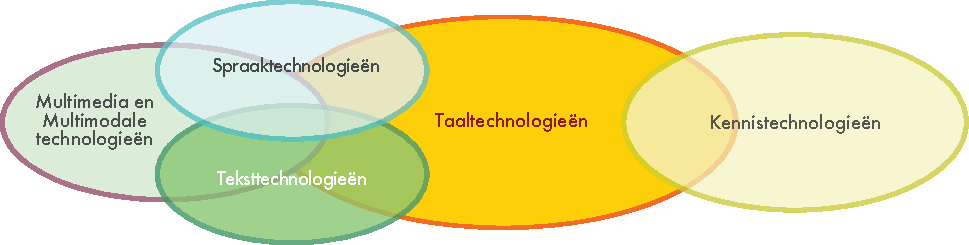
\includegraphics[width=\textwidth]{../_media/dutch/language_technologies}
  \caption{XXX Sprachtechnologie im Kontext}
  \label{fig:ltincontext_nl}
  \colorrule{grey3}{\textwidth}{1.5pt}
\end{figure*}


Bij onze communicatie vermengen we taal met andere manieren van communicatie en met andere informatiemedia. We combineren spraak met gebaren en gezichtsuitdrukkingen. Digitale teksten worden gecombineerd met plaatjes en geluiden. Films kunnen taal in gesproken en geschreven vorm bevatten. Daarom overlappen spraak- en teksttechnologie{\"e}n en interageren zij met vele andere technologie{\"e}n die het verwerken van multimodale communicatie en multimedia documenten vergemakkelijken.

XXX
Im Folgenden werden wir uns mit den Hauptanwendungsbereichen der Sprachtechnologie beschäftigen, insbesondere mit Sprachüberprüfung, Websuche, Sprach\-inter\-aktion und maschineller Übersetzung. Dies umfasst Anwendungen und Basistechnologien wie beispielsweise

\begin{itemize}
\item Rechtschreibkorrektur
\item Unterstützung bei der Texterstellung
\item Computergestützter Spracherwerb
\item Informationssuche
\item Informationsextraktion
\item Textzusammenfassung
\item Frage-Antwort-Systeme
\item Spracherkennung 
\item Sprachsynthese
\end{itemize}

Sprachtechnologie ist ein etabliertes Forschungsgebiet mit weitreichender Grundlagenliteratur. Der interessierte Leser sei auf \cite{carstensen-etal1, jurafsky-martin01, manning-schuetze1, lt-world1, lt-survey1} verwiesen.

Bevor wir die oben genannten Anwendungsbereiche genauer behandeln, werden wir zunächst die Architektur eines typischen sprachtechnologischen Systems beschreiben. 
XXX

\subsection[Toepassingsarchitecturen voor Taaltechnologie]{Toepassingsarchitecturen voor Taaltechnologie}

Typische softwaretoepassingen voor taalverwerking bestaan uit meerdere componenten die verschillende aspecten reflecteren van taal en de taak die zij implementeren. De illustratie~\ref{fig:textprocessingarch_de} laat een sterk vereenvoudigde architectuur zien die in een tekstverwerkingssysteem gevonden wordt. De eerste drie modules behandelen de structuur en de betekenis van de tekstinput:
\begin{figure*}[b]
  \colorrule{grey3}{\textwidth}{1.5pt}
  \center
  %\vspace{-5mm} 
  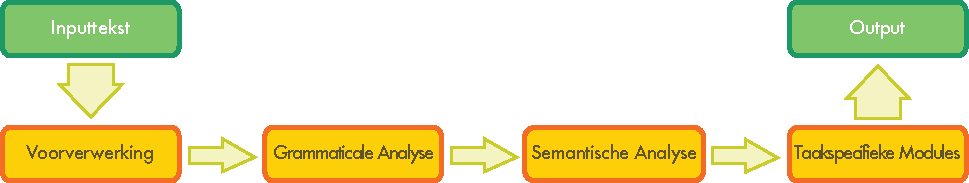
\includegraphics[width=\textwidth]{../_media/dutch/text_processing_app_architecture}
  \caption{Een Typische Toepassingsarchitectuur voor Tekstverwerking}
  \label{fig:textprocessingarch_de}
  \colorrule{grey3}{\textwidth}{1.5pt}
\end{figure*}
%
    \begin{enumerate}
 	\item Voorverwerking: opschonen van de data, het verwijderen van opmaak, detecteren wat de input taal is, "e" door "{\"e}" vervangen (in het Nederlands), etc.
 	\item Grammaticale analyse: het werkwoord en zijn complementen vinden, bepalingen, etc.; de zinsstructuur vaststellen.
 	\item Semantische analyse: desambiguering: Welke betekenis van \emph{appel} is de juiste in de gegeven context?, de verwijzing van voornaamwoorden zoals \emph{zij} en van uitdrukkingen zoals \emph{de auto} oplossen, etc.; de betekenis van de zin weergeven op een voor machines leesbare manier
    \end{enumerate}
%
    Taakspecifieke modules voeren dan allerlei operaties uit zoals automatische samenvatting van een inputtekst, zoeken in een databank en vele andere. Beneden zullen we \textbf{kerntoepassingsgebieden} illustreren en enkele van de modules van de verschillende architecturen in iedere sectie voor het voetlicht brengen. De architecturen zoals hier geschetst zijn sterk vereenvoudigd en ge{\"\i}dealiseerd, en dienen vooral om de complexiteit van taaltechnologische toepassingen op een algemeen begrijpelijke manier duidelijk te maken.

    Na de introductie van de kerntoepassingsgebieden zullen we een kort overzicht geven van de situatie in taaltechnologieonderzoek en -onderwijs, en we sluiten af met een overzicht van (in het verleden) gefinancierde programma's. Tot slot presenteren we, in tabelvorm, een inschatting door experts van de situatie met betrekking tot essenti{\"e}le taaltechnologische software en data langs een aantal dimensies, zoals beschikbaarheid, maturiteit, en kwaliteit (XXX Abbildung~\ref{fig:lrlttable_de}) . Deze tabel geeft een goed overzicht van de situatie voor taaltechnologie voor het Nederlands.

XXX
im Text fett gedruckte Anwendungen und Ressourcen sind ebenfalls in dieser Abbildung zu finden. Im Anschluss wird das Deutsche im Hinblick auf die sprachtechnologische Unterstützung mit anderen Sprachen verglichen, die im Rahmen dieser Weißbuchserie untersucht wurden.


\subsection{Kerntoepassingsgebieden} 

%In diesem Abschnitt konzentrieren wir uns auf die wichtigsten sprachtechnologischen Anwendungen und Ressourcen und geben einen Überblick über Aktivitäten im Bereich Sprachtechnologie in Deutschland, Österreich und in der Schweiz. 


\begin{figure*}[t]
  \colorrule{grey3}{\textwidth}{1.5pt}
 % \vspace{-9mm}
  \center
  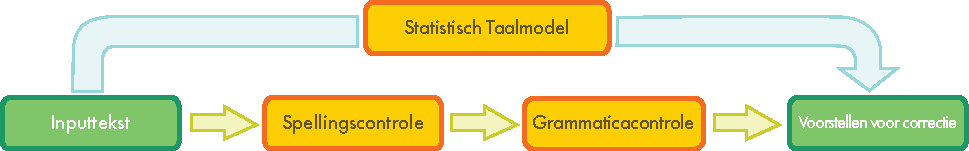
\includegraphics[width=\textwidth]{../_media/dutch/language_checking}
  \caption{Taalcontrole (links: regelgebaseerd, rechts: statistisch)}
  \label{fig:langcheckingaarch_de}
  \colorrule{grey3}{\textwidth}{1.5pt}
\end{figure*}


\subsubsection{Taalcontrole}

    Iedereen die een tekstverwerker gebruikt zoals Microsoft Word is wel een component voor spellingscontrole tegengekomen die spellingsfouten aanduidt en verbeteringen suggereert. Veertig jaar na het eerste programma voor spellingscorrectie door Ralph Gorin vergelijken taalcontroleprogramma's niet meer eenvoudigweg de lijst van gevonden woorden tegen een woordenboek van correct gespelde woorden: zij zijn aanzienlijk gesofisticeerder geworden. Naast taalspecifieke algoritmes om met morfologie (bijv. meervoudsvormen) om te gaan, kunnen sommige ook bepaalde syntactische fouten herkennen, zoals een ontbrekend werkwoord of een werkwoord dat niet congrueert met het onderwerp in persoon en getal, bijv. in \emph{Hij *bied geld aan}. De meeste spellingscontroleprogramma's (inclusief Microsoft Word) vinden echter geen fouten in de volgende tekst \cite{zar1}:


\begin{quote}
  I have a spelling checker,\\
  It came with my PC.\\
  It plane lee marks four my revue\\
  Miss steaks aye can knot sea.
\end{quote}



    Om met dit soort fouten om te gaan is in veel gevallen een analyse van de context nodig, bijvoorbeeld om te beslissen of een werkwoord in het Nederlands geschreven moet worden met \emph{dt} of \emph{d}, zoals in:

\begin{itemize}
 \item   Hij heeft het dier \underline{verwond}.
 \item   Hij \underline{verwondt} het dier.
\end{itemize}



    Dit vereist hetzij de formulering van taalspecifieke grammaticaregels, d.w.z. een hoge mate van expertise en manueel werk, hetzij het gebruik van een zogenaamd statistisch taalmodel. Zulke modellen berekenen de waarschijnlijkheid van het voorkomen van een bepaald woord in een specifieke context (d.w.z. de woorden ervoor en erna). Zo is bijvoorbeeld \emph{hij verwondt} een veel waarschijnlijkere woordsequentie dan \emph{hij verwond}. Een statistisch taalmodel kan automatisch worden afgeleid van een grote hoeveelheid (correcte) taaldata (d.w.z., een corpus) (XXXsiehe Abbildung~\ref{fig:langcheckingaarch_de}). Tot nu toe zijn deze benaderingen het meest toegepast en ge{\"e}valueerd op Engelse taaldata. Maar ze zijn niet per se eenvoudig over te zetten naar het Nederlands met zijn flexibelere woordvolgorde, combinaties van werkwoorden en scheidbare prefixen, samenstellingen, en kruisende afhankelijkheden.

\boxtext{XXX Der Einsatz der Sprachprüfung ist nicht auf Textverarbeitungsprogramme beschränkt. Sie ist auch zur Autorenunterstützung anwendbar.}

    Het gebruik van taalcontrolesoftware is niet beperkt tot tekstverwerkers, maar kan ook toegepast worden in systemen voor auteursondersteuning. Met het stijgende aantal technische producten is in de laatste decennia ook de hoeveelheid technische documentatie snel toegenomen. Uit angst voor klachten van klanten over verkeerd gebruik en schadeclaims voortkomend uit slechte of slecht begrepen instructies, zijn bedrijven meer en meer begonnen zich te richten op de kwaliteit van technische documentatie, terwijl ze tegelijkertijd de internationale markt bedienen. Vooruitgang in de verwerking van natuurlijke taal hebben geleid tot de ontwikkeling van software voor auteursondersteuning, die de schrijver van technische documentatie assisteert om vocabulaire en zinsstructuren te gebruiken die consistent zijn met bepaalde regels en (bedrijfs)specifieke terminologiebeperkingen.



    Spellingscontrolesoftware voor het Nederlands ge{\"\i}ncorporeerd in Microsoft producten zijn in het verleden ontwikkeld door Lernout \& Hauspie, onafhankelijk later ook door Polderland, en deze soft-ware wordt momenteel onderhouden en verder ontwikkeld door Knowledge Concepts. Andere bedrijven actief op dit gebied zijn *TAL{\=O} BV en Carp Technologies.

    Naast spellingcontrole en auteursondersteuning is taalcontrole ook van belang op het gebied van computerondersteund taalonderwijs en wordt het toegepast om automatisch zoekopdrachten verstuurd naar zoekmachines op het web te corrigeren, bijvoorbeeld de `Bedoelt u�' suggesties van Google.

\subsubsection{Zoeken op het Web}

 Zoeken op het web, in een intranet, of in digitale bibliotheken is vandaag waarschijnlijk de meest gebruikte maar toch nog onderontwikkelde taaltechnologie. De zoekmachine Google, die begon in 1998, wordt tegenwoordig wereldwijd voor ongeveer 80\% van alle zoekopdrachten gebruikt \cite{Spiegel}. Het werkwoord \emph{googelen} is zelfs opgenomen in het Nederlandse Van Dale woordenboek. Noch de zoekinterface, noch de presentatie van de verkregen resultaten is significant veranderd sinds de eerste versie. In de huidige versie biedt Google spellingscorrectie voor verkeerd gespelde woorden en het incorporeerde ook, in 2009, een basisversie van semantische zoekfunctionaliteit in hun algoritmische mix \cite{GoogleSem}, die de accuraatheid van het zoeken kan verbeteren door de betekenis van de zoektermen in context te analyseren. Het succesverhaal van Google toont aan dat met de beschikbaarheid van een grote hoeveelheid data en effici{\"e}nte technieken voor het indexeren van deze data, een grotendeels statistisch gebaseerde benadering tot bevredigende resultaten kan leiden.

\begin{figure*}[tb]
  \colorrule{grey3}{\textwidth}{1.5pt}
  \vspace{-9mm}
  \center
  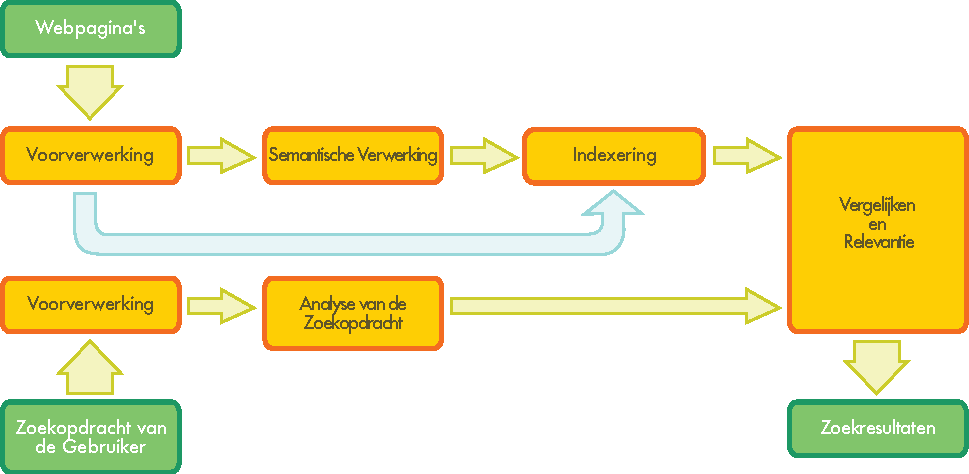
\includegraphics[width=\textwidth]{../_media/dutch/web_search_architecture}
  \vspace{-5mm}
  \caption{Architectuur voor Zoeken op het Web}
  \label{fig:websearcharch_de}
  \colorrule{grey3}{\textwidth}{1.5pt}
\end{figure*}

    Voor een meer gesofisticeerd verzoek om informatie is echter de integratie van diepere taalkundige kennis essentieel. In de onderzoekslaboratoria hebben experimenten met voor machines leesbare thesauri en ontologische taalbronnen zoals WordNet (of het equivalent EuroWordNet Nederlands), verbeteringen laten zien door het mogelijk te maken een pagina te vinden op basis van synoniemen van de zoektermen, bijv. \emph{kernenergie} en \emph{nucleaire energie}, of zelfs losser gerelateerde termen.

    De volgende generatie zoekmachines zal meer gesofisticeerde taaltechnologie moeten bevatten. Als een zoekopdracht bestaat uit een vraag of een ander type zin dan simpelweg een lijstje trefwoorden, dan vereist het ophalen van relevante antwoorden voor deze zoekopdracht een analyse van deze zin op syntactisch en semantisch niveau (XXX siehe Abbildung~\ref{fig:websearcharch_de}) evenals de beschikbaarheid van een index die het mogelijk maakt snel de relevante documenten op te halen. Stelt u zich bijvoorbeeld voor dat een gebruiker als zoekopdracht ingeeft: `Geef me een lijst van alle bedrijven die overgenomen zijn door andere bedrijven in de laatste vijf jaar'. Voor een bevredigend antwoord moet er syntactische ontleding (parsing) toegepast worden om de grammaticale structuur van de zin te analyseren en te bepalen dat de gebruiker zoekt naar bedrijven die overgenomen zijn en niet bedrijven die overgenomen hebben. Ook de uitdrukking \emph{in de laatste vijf jaar} moet verwerkt worden om te bepalen naar welke jaren het precies verwijst.

    Tot slot moet de verwerkte zoekopdracht vergeleken worden met een gigantische hoeveelheid ongestructureerde data om het stukje of de stukjes informatie te vinden waar de gebruiker naar zoekt. Dit wordt gewoonlijk \emph{information retrieval} genoemd en omvat het zoeken naar en rangschikken van relevante documenten. Bovendien moeten we om een lijst van bedrijven te genereren ook de informatie extraheren dat een bepaalde karakterreeks in een document verwijst naar de naam van een bedrijf. Dat soort informatie wordt beschikbaar gemaakt door herkenning van benoemde entiteiten met behulp van zogenaamde named-entity recognizers.

    Nog meer eisen stelt de poging een zoekopdracht te vergelijken met documenten geschreven in een andere taal. Voor zulke \emph{cross-lingual information retrieval} moeten we de zoekopdracht automatisch vertalen naar alle mogelijke brontalen en de opgehaalde informatie terugvertalen naar de doeltaal. Het toenemend percentage data dat beschikbaar is in andere vormen dan tekst drijft de vraag naar diensten die information retrieval in multimedia mogelijk maken, d.w.z., het zoeken naar informatie in beeld-, audio-, en videodata. Voor audio- en videobestanden is daarvoor een spraakherkenningsmodule vereist om gesproken inhoud om te zetten in een tekstuele of fonetische representatie waar zoekopdrachten van de gebruiker mee vergeleken kunnen worden.

    In Nederland zijn verschillende bedrijven actief op deze gebieden, waaronder AskNow Solutions, Carp Technologies, GridLine, Irion Technologies, Knowledge Concepts, MediaLab Solutions, RightNow! (voorheen Q-Go), TextKernel, en andere. In Belgi{\"e} zijn Natlanco, InterSystems (voorheen i.Know), ICMS, Aktor Technologies, Mentoring Systems en CrossMinder actief op deze gebieden.

    De focus van de ontwikkeling ligt voor deze bedrijven in het leveren van bijkomende functionaliteit en geavanceerde zoekmachines voor portalen gericht op specifieke onderwerpen door gebruik te maken van onderwerpsrelevante semantiek. Vanwege de steeds nog hoge vereisten aan verwerkingskracht zijn zulke zoekmachines alleen economisch rendabel op relatief kleine tekstcorpora. De benodigde verwerkingstijd gaat al snel die van een gewone statistische zoekmachine (bijv. Google) met een factor van een ordegrootte van enkele duizenden te boven. Deze zoekmachines stellen ook hoge eisen aan onderwerpspecifieke domeinmodellering, waardoor het niet mogelijk is ze te gebruiken op de schaal van het web.
  
\subsubsection{Spraakinteractie}

  Spraakinteractie is een van de vele toepassingsgebieden die afhankelijk zijn van spraaktechnologie, d.w.z. technologie{\"e}n om gesproken taal te verwerken. Spraaktechnologie wordt gebruikt om interfaces te cre{\"e}ren die een gebruiker in staat stellen te werken met machines via gesproken taal in plaats van via een grafisch scherm, een toetsenbord, en een muis. Vandaag de dag worden deze stemgestuurde interfaces (`voice user interfaces', VUIs) gebruikt voor het gedeeltelijk of geheel automatiseren van diensten die aangeboden worden door bedrijven aan hun klanten, medewerkers, of partners via de telefoon (XXX siehe Abbildung~\ref{fig:dialoguearch_de}). Bedrijfsdomeinen die een grootschalig beroep doen op VUIs zijn bankieren, logistiek, openbaar vervoer, en telecommunicatie. Spraaktechnologie wordt ook gebruikt als interface naar specifieke apparaten, bijv. navigatiesystemen in de auto, en als alternatief voor de input/output modaliteiten van grafische  gebruikersinterfaces, bijv.  in `smart phones', d.w.z. intelligente mobiele telefoons.

\boxtext{Sprachtechnologie ermöglicht Schnittstellen, über die ein Nutzer mittels gesprochener Sprache interagieren kann.}

\begin{figure*}[htb]
  \colorrule{grey3}{\textwidth}{1.5pt}
  %\vspace{-9mm}
  \center  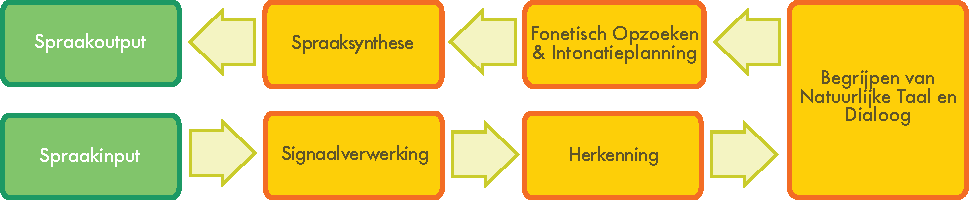
\includegraphics[width=\textwidth]{../_media/dutch/simple_speech-based_dialogue_architecture}
  \center
  \caption{Simpele Spraakgebaseerde Dialoogarchitectuur}
  \label{fig:dialoguearch_de}
  \colorrule{grey3}{\textwidth}{1.5pt}
\end{figure*}

    Spraakinteractie omvat vier technologie{\"e}n:
    \begin{enumerate}
    \item Automatische spraakherkenning (`automatic speech recognition', ASR) bepaalt welke woorden feitelijk uitgesproken worden op basis van een sequentie van geluiden geuit door een gebruiker.
 	\item Syntactische analyse en semantische interpretatie houden zich bezig met de syntactische structuur van de uiting van de gebruiker en het interpreteren ervan in overeenstemming met het doel van het systeem.
 	\item Dialoogmanagement zorgt ervoor dat het systeem waar de gebruiker mee werkt kan bepalen welke actie ondernomen moet worden gegeven de input van de gebruiker en de functionaliteit van het systeem.
 	\item Spraaksynthese (ook wel tekst-naar-spraak `Text-to-Speech', TTS): deze technologie wordt ingezet om de verwoording van een uiting om te zetten in spraakgeluid dat dient als uitvoer van het systeem en als invoer voor de gebruiker
    \end{enumerate}

    Het is een van de grote uitdagingen om een ASR-systeem te maken dat de woorden die geuit worden door een gebruiker zo precies mogelijk herkent. Dit is moeilijk omdat spraak geen spaties bevat tussen woorden (zoals in de geschreven taal), en omdat het spraaksignaal zeer variabel van karakter is (accentverschillen, mannenstemmen verschillen van vrouwenstemmen, achtergrondgeluiden, etc.). Dit vereist {\`o}f een beperking op de reeks van mogelijke gebruikersuitingen tot een beperkte set van trefwoorden, {\`o}f het manueel aanmaken van taalmodellen die een grote reeks natuurlijke gebruikersuitingen afdekt. Het eerste alternatief resulteert in een nogal rigide en inflexibel gebruik van een VUI en misschien ook in slechte gebruikersacceptatie. In het tweede alternatief kan het cre{\"e}ren, afstemmen en onderhouden van taalmodellen de kosten behoorlijk opdrijven. VUIs die taalmodellen gebruiken en het de gebruiker toestaan zijn/haar bedoeling op flexibele manier uit te drukken --- opgeroepen door bijvoorbeeld een `Hoe kan ik u helpen' begroeting --- vertonen een hogere automatiseringsgraad en een grotere gebruikersacceptatie en kunnen daarom beschouwd worden als bevoordeeld boven een minder flexibele gestuurde dialoogbenadering.

    Voor het outputgedeelte van een VUI plegen bedrijven heel vaak van te voren opgenomen uitingen van professionele --- idealiter met het bedrijf geassocieerde --- sprekers te gebruiken. Voor statische uitingen waar de verwoording niet afhangt van de specifieke context of de persoonlijke gegevens van de gebruiker, zal dit resulteren in een rijke gebruikerservaring. Maar hoe meer een uiting dynamische inhoud in ogenschouw moet nemen, hoe meer de gebruikerservaring zal lijden onder een slechte prosodie die resulteert uit het achter elkaar zetten van audiobestanden. De TTS-systemen van tegenwoordig daarentegen, blijken superieur op het gebied van de prosodische natuurlijkheid van dynamische uitingen, ook al zijn verbeteringen zeker nog mogelijk.

    Kijken we naar de markt voor spraakinteractie, dan zien we dat in het laatste decennium een sterke standaardisatie van de interfaces tussen de verschillende technologiecomponenten is opgetreden. Dat geldt ook voor standaarden voor het cre{\"e}ren van bepaalde softwareartefacten voor een gegeven toepassing. Er is ook sprake geweest van een sterke marktconsolidatie in de laatste tien jaar, vooral op het gebied van ASR en TTS. Hier worden de nationale markten in de G20-landen -- d.w.z. economisch sterke landen met een aanzienlijke bevolking -- gedomineerd door minder dan vijf spelers wereldwijd, met Nuance (V.S.) en Loquendo (Itali{\"e}) als meest prominente spelers in Europa. Nuance heeft een groot ontwikkelingscentrum in Vlaanderen.

    Op de Nederlandse TTS-markt zijn er ook nog kleinere bedrijven zoals Acapela, gebaseerd in Walloni{\"e}, SVOX, met het hoofdkwartier in Zwitserland, en Fluency, gebaseerd in Amsterdam. Er zijn veel bedrijven die TTS en ASR technologie integreren in toepassingen en diensten. Hieronder vallen Advance Voice Technology, DB-Scape, Dialogs Unlimited, DutchEar,   G2 Speech,  Logica, OrcaVoice, Quentris, Telecats, TomTom en Voice Data Bridge. Verschillende bedrijven en stichtingen richten zich op toepassingen voor gebruikersgroepen met speciale eisen zoals fysiek gehandicapten, dyslectici, en ouderen. Daaronder vallen Axendo, Cochlear Benelux, Dedicon, JABBLA, Kamelego, Lexima, rdgKompagne, Sensotec NV en VoiceCore.

    Met betrekking tot technologie en kennis voor dialoogmanagement zijn enkele relevante bedrijven Carp Technologies, Irion, RightNow! (voorheen Q-Go) en  RE-Phrase voor tekstgebaseerde toepassingen, en  Dialogs Unlimited, DutchEar, Telecats, en Voice Data Bridge  voor spraakgebaseerde toepassingen. Op het gebied van de spraakinteractie bestaat er nog geen echte markt voor de taalkundige kerntechnologie{\"e}n voor syntactische en semantische analyse.

    Wat betreft het daadwerkelijk gebruik van VUIs is de vraag de laatste vijf jaar toegenomen. Deze tendens werd gedreven door de toenemende vraag van eindgebruikers naar `zelfbediening' door de klant, door het feit dat er een behoorlijke kostenoptimalisatie verkregen kon worden met geautomatiseerde telefoondiensten, en verder door een significant toegenomen acceptatie van gesproken taal als een modaliteit voor mens-machine interactie.

    Kijken we voorbij de huidige stand van de techniek, dan zien we significante veranderingen dankzij de verspreiding van `smart phones' als een nieuw platform voor het onderhouden van klantenrelaties - naast de telefoon-, internet- en e-mailkanalen. Deze tendens zal ook het gebruik van spraaktechnologie be{\"\i}nvloeden. Enerzijds zal de vraag naar telefoongebaseerde VUIs op de lange termijn afnemen. Anderzijds zal het gebruik van gesproken taal als een gebruikersvriendelijke inputmodaliteit voor `smart phones' behoorlijk aan belang winnen. Deze tendens wordt ondersteund door de waarneembare verbetering van de accuraatheid van sprekeronafhankelijke spraakherkenning voor spraakdicteerdiensten die al aangeboden worden als gecentraliseerde diensten aan gebruikers van `smart phones'. Met dit `uitbesteden' van de herkenningstaak naar de toepassingsinfrastructuur, zal, naar verondersteld wordt, het applicatiespecifieke gebruik van essenti{\"e}le taalkundige technologie{\"e}n aan belang winnen in vergelijking met de huidige situatie.

\subsubsection{Automatisch Vertalen}

  Het idee om digitale computers te gebruiken voor het vertalen van natuurlijke talen ontstond in 1946 bij A. D. Booth en werd gevolgd door een substanti{\"e}le financiering van onderzoek op dit gebied in de jaren vijftig en opnieuw in de jaren tachtig van de vorige eeuw. Desondanks kan automatisch vertalen (Machine Translation, MT) nog steeds de hoge verwachtingen die het in de eerste jaren wekte niet inlossen.

    In de eenvoudigste vorm vervangt MT simpelweg woorden in de ene natuurlijke taal door corresponderende woorden in een andere natuurlijke taal. Dit kan nuttig zijn in onderwerpsdomeinen met heel beperkte, formuleachtige taal, bijv. in weerberichten. Maar voor een goede vertaling van minder gestandaardiseerde teksten moeten grotere teksteenheden (woordgroepen, zinnen, of zelfs hele passages) vergeleken worden met hun dichtstbijzijnde tegenhangers in de doeltaal. Het grote probleem hierbij is dat natuurlijke taal ambigu is, wat uitdagingen stelt op meerdere niveaus, bijv. desambiguering van woordbetekenissen op het lexicale niveau (bijv. \emph{graven} kan staan voor `mensen met een specifieke adellijke titel', `laatste rustplaatsen' of `grond wegscheppen'), of de interpretatie van betrekkelijke voornaamwoorden (als onderwerp of als lijdend voorwerp) op het syntactische niveau, zoals in:\\

    \emph{De man die de vrouw zag}\\

    E{\'e}n manier om deze taak te benaderen is gebaseerd op taalkundige regels. Voor vertaling tussen nauw verwante talen is een directe vertaling misschien mogelijk voor simpele gevallen. Maar vaak is het nodig dat een regelgebaseerd (of kennisgedreven) systeem de ingevoerde tekst analyseert en een intermediaire symbolische representatie maakt van waaruit de tekst in de doeltaal gegenereerd wordt. Het succes van deze methodes is sterk afhankelijk van de beschikbaarheid van uitgebreide lexicons met morfologische, syntactische, en semantische informatie, en grote verzamelingen van grammaticaregels die zorgvuldig ontworpen zijn door een vaardig taalkundige.

\begin{figure*}[htb]
  \colorrule{grey3}{\textwidth}{1.5pt}
  \vspace{-21mm}
  \center
  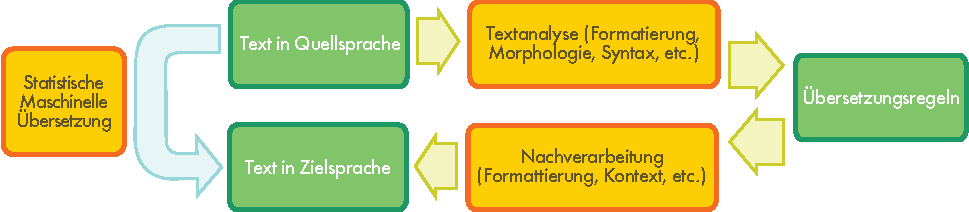
\includegraphics[width=\textwidth]{../_media/german/machine_translation}
  \vspace{-2mm}
  \caption{Automatisch Vertalen (boven: statistisch, onder: regelgebaseerd)}
  \label{fig:mtarch_de}
  \colorrule{grey3}{\textwidth}{1.5pt}
\end{figure*}

    Vanaf de late jaren tachtig van de vorige eeuw kwam er, aangezien de computationele kracht toenam en minder duur werd, meer belangstelling voor statistische modellen voor MT. De parameters van deze statistische modellen worden afgeleid uit de analyse van tweetalige tekstcorpora, zoals het \emph{Europarl} parallelle corpus, dat de notulen van het Europees Parlement bevat in 11 Europese talen. Als er genoeg data zijn werkt statistische MT goed genoeg om een benadering van de betekenis van een tekst in een vreemde taal te verkrijgen. Maar, in tegenstelling tot kennisgedreven systemen, produceert statistische (of datagedreven) MT vaak ongrammaticale output. Anderzijds kan datagedreven MT, naast het voordeel dat minder menselijke inspanning vereist is voor het schrijven van de grammatica, ook eigenaardigheden van de taal die minder makkelijke te vangen zijn in kennisgedreven systemen afdekken, zoals idiomatische uitdrukkingen.

    Aangezien de sterktes en zwaktes van de kennis- en datagedreven MT (XXX siehe Abbildung~\ref{fig:mtarch_de}) complementair zijn, richten onderzoekers zich tegenwoordig unaniem op hybride benaderingen waarin methodologie{\"e}n van beide gecombineerd worden. Dit kan op verschillende manieren gedaan worden. E{\'e}n mogelijkheid is om zowel kennisgedreven als datagedreven systemen te gebruiken en een selectiemodule de beste output te laten kiezen voor iedere zin. Voor langere zinnen zal echter geen enkel resultaat perfect zijn. Een betere oplossing is het om de beste delen van zinnen van meervoudige output te combineren, maar dat kan behoorlijk complex zijn omdat niet altijd evident is welke delen van meervoudige alternatieven corresponderen en gealigneerd moeten worden.

\boxtext{XXX Maschinelle Übersetzung stellt bei der deutschen Sprache eine besondere Herausforderung dar.} 

    Voor het Nederlands is MT bijzonder uitdagend. De mogelijkheid om willekeurig nieuwe woorden te cre{\"e}ren door samenstelling maakt woordenboekanalyse en woordenboekafdekking moeilijk; relatief vrije woordvolgorde, gespleten werkwoordconstructies en R-pronomina zijn eveneens problematisch voor analyse.

    Leidende commerci{\"e}le MT-systemen uit het verleden zoals Systran, Globalink, LOGOS, METAL (en zijn spin-offs, LANT (tegenwoordig Xplanation), GMS and Lucy Software), en LMT ontwikkeld door IBM (dat de basis vormt voor Linguatec en Lingenio), dekten nooit het Nederlands af, waarschijnlijk om dat het niet interessant was vanuit commercieel oogpunt. Er werden alleen wat onderzoekssystemen ontwikkeld voor het Nederlands, gedeeltelijk in bedrijven (Philips: Rosetta, BSO: Distributed Translation) en gedeeltelijk in de academische wereld (Universiteit Utrecht \& KU Leuven: Eurotra). Vertaalsystemen voor het Nederlands werden alleen ontwikkeld wanneer dit gefinancierd werd met publiek geld. Zo ontwikkelde METAL een Nederlands-Frans MT-systeem voor de ministeries van landbouw en binnenlandse zaken, en na een oproep door de Nederlandse Taalunie in 1999 voor de ontwikkeling van een MT-systeem dat vertaalt tussen Nederlands aan de ene kant en Frans en Engels aan de andere kant \cite{Cucchiarini:etal:2000}, ontwikkelde Systran dergelijke systemen in de context van het NL-Translex project.

    Alle bovengenoemde systemen waren kennisgebaseerd. Met de opkomst van statistische MT is het Nederlands een vrij algemeen afgedekt taal geworden. Het behoort bij de 52 talen die Google Translate aanbiedt en bij de 24 talen die SDL Language Weaver aanbiedt.

    Indien een MT-systeem goed aangepast is naar gebruikersspecifieke terminologie en goed ge{\"\i}ntegreerd is in bedrijfsprocessen, kan het gebruik van MT de productiviteit flink opdrijven. De meeste MT-bedrijven benadrukken dat zij hun standaardsystemen snel kunnen aanpassen naar bedrijfsspecifieke woordenboeken, terminologie en vertaalgeheugens en daarmee de kwaliteit van MT significant kunnen verbeteren.

    De kwaliteit van MT-systemen kan nog flink verbeteren. Uitdagingen hierbij omvatten de aanpasbaarheid van de taalbronnen aan een gegeven onderwerps- of gebruikersgebied en integratie in bestaande bedrijfsprocessen met termbanken en vertaalgeheugens. Bovendien zijn de meeste huidige systemen op het Engels geori{\"e}nteerd en ondersteunen zij slechts enkele talen met directe vertaling van of naar het Nederlands, wat leidt tot spanningen in het hele vertaalproces, en bijvoorbeeld gebruikers van MT dwingt voor ieder nieuw systeem een ander tool te leren voor het coderen van lexicons.

\begin{figure*}[tb]
  \centering
  \setlength{\tabcolsep}{0.17em}
  \small
  \begin{tabular}{>{\columncolor{corange1}}cccccccccccccccccccccccc}
    & \multicolumn{22}{>{\columncolor{corange1}}c}{Zielsprache -- \textcolor{grey1}{Target language}}\\\addlinespace[{-.009cm}]
    \rowcolor{corange1}  & EN & BG & DE & CS & DA & EL & ES & ET & FI & FR & HU & IT & LT & LV & MT & NL & PL & PT & RO & SK & SL & SV\\
    EN & -- & \textcolor{blue}{40.5} & \textcolor{blue}{46.8} & \textcolor{green2}{52.6} & \textcolor{green2}{50.0} & \textcolor{blue}{41.0} & \textcolor{green2}{55.2} & \textcolor{purple}{34.8} & \textcolor{purple}{38.6} & \textcolor{green2}{50.1} & \textcolor{purple}{37.2} & \textcolor{green2}{50.4} & \textcolor{purple}{39.6} & \textcolor{blue}{43.4} & \textcolor{purple}{39.8} & \textcolor{green2}{52.3} & \textcolor{blue}{49.2} & \textcolor{green2}{55.0} & \textcolor{blue}{49.0} & \textcolor{blue}{44.7} & \textcolor{green2}{50.7} & \textcolor{green2}{52.0}\\
    BG & \textcolor{green}{61.3} & -- & \textcolor{purple}{38.7} & \textcolor{purple}{39.4} & \textcolor{purple}{39.6} & \textcolor{purple}{34.5} & \textcolor{blue}{46.9} & \textcolor{red3}{25.5} & \textcolor{red3}{26.7} & \textcolor{blue}{42.4} & \textcolor{red3}{22.0} & \textcolor{blue}{43.5} & \textcolor{red3}{29.3} & \textcolor{red3}{29.1} & \textcolor{red3}{25.9} & \textcolor{blue}{44.9} & \textcolor{purple}{35.1} & \textcolor{blue}{45.9} & \textcolor{purple}{36.8} & \textcolor{purple}{34.1} & \textcolor{purple}{34.1} & \textcolor{purple}{39.9}\\
    DE & \textcolor{green2}{53.6} & \textcolor{red3}{26.3} & -- & \textcolor{purple}{35.4} & \textcolor{blue}{43.1} & \textcolor{purple}{32.8} & \textcolor{blue}{47.1} & \textcolor{red3}{26.7} & \textcolor{red3}{29.5} & \textcolor{purple}{39.4} & \textcolor{red3}{27.6} & \textcolor{blue}{42.7} & \textcolor{red3}{27.6} & \textcolor{purple}{30.3} & \textcolor{red2}{19.8} & \textcolor{green2}{50.2} & \textcolor{purple}{30.2} & \textcolor{blue}{44.1} & \textcolor{purple}{30.7} & \textcolor{red3}{29.4} & \textcolor{purple}{31.4} & \textcolor{blue}{41.2}\\
    CS & \textcolor{green2}{58.4} & \textcolor{purple}{32.0} & \textcolor{blue}{42.6} & -- & \textcolor{blue}{43.6} & \textcolor{purple}{34.6} & \textcolor{blue}{48.9} & \textcolor{purple}{30.7} & \textcolor{purple}{30.5} & \textcolor{blue}{41.6} & \textcolor{red3}{27.4} & \textcolor{blue}{44.3} & \textcolor{purple}{34.5} & \textcolor{purple}{35.8} & \textcolor{red3}{26.3} & \textcolor{blue}{46.5} & \textcolor{purple}{39.2} & \textcolor{blue}{45.7} & \textcolor{purple}{36.5} & \textcolor{blue}{43.6} & \textcolor{blue}{41.3} & \textcolor{blue}{42.9}\\
    DA & \textcolor{green2}{57.6} & \textcolor{red3}{28.7} & \textcolor{blue}{44.1} & \textcolor{purple}{35.7} & -- & \textcolor{purple}{34.3} & \textcolor{blue}{47.5} & \textcolor{red3}{27.8} & \textcolor{purple}{31.6} & \textcolor{blue}{41.3} & \textcolor{red3}{24.2} & \textcolor{blue}{43.8} & \textcolor{red3}{29.7} & \textcolor{purple}{32.9} & \textcolor{red3}{21.1} & \textcolor{blue}{48.5} & \textcolor{purple}{34.3} & \textcolor{blue}{45.4} & \textcolor{purple}{33.9} & \textcolor{purple}{33.0} & \textcolor{purple}{36.2} & \textcolor{blue}{47.2}\\
    EL & \textcolor{green2}{59.5} & \textcolor{purple}{32.4} & \textcolor{blue}{43.1} & \textcolor{purple}{37.7} & \textcolor{blue}{44.5} & -- & \textcolor{green2}{54.0} & \textcolor{red3}{26.5} & \textcolor{red3}{29.0} & \textcolor{blue}{48.3} & \textcolor{red3}{23.7} & \textcolor{blue}{49.6} & \textcolor{red3}{29.0} & \textcolor{purple}{32.6} & \textcolor{red3}{23.8} & \textcolor{blue}{48.9} & \textcolor{purple}{34.2} & \textcolor{green2}{52.5} & \textcolor{purple}{37.2} & \textcolor{purple}{33.1} & \textcolor{purple}{36.3} & \textcolor{blue}{43.3}\\
    ES & \textcolor{green}{60.0} & \textcolor{purple}{31.1} & \textcolor{blue}{42.7} & \textcolor{purple}{37.5} & \textcolor{blue}{44.4} & \textcolor{purple}{39.4} & -- & \textcolor{red3}{25.4} & \textcolor{red3}{28.5} & \textcolor{green2}{51.3} & \textcolor{red3}{24.0} & \textcolor{green2}{51.7} & \textcolor{red3}{26.8} & \textcolor{purple}{30.5} & \textcolor{red3}{24.6} & \textcolor{blue}{48.8} & \textcolor{purple}{33.9} & \textcolor{green2}{57.3} & \textcolor{purple}{38.1} & \textcolor{purple}{31.7} & \textcolor{purple}{33.9} & \textcolor{blue}{43.7}\\
    ET & \textcolor{green2}{52.0} & \textcolor{red3}{24.6} & \textcolor{purple}{37.3} & \textcolor{purple}{35.2} & \textcolor{purple}{37.8} & \textcolor{red3}{28.2} & \textcolor{blue}{40.4} & -- & \textcolor{purple}{37.7} & \textcolor{purple}{33.4} & \textcolor{purple}{30.9} & \textcolor{purple}{37.0} & \textcolor{purple}{35.0} & \textcolor{purple}{36.9} & \textcolor{red3}{20.5} & \textcolor{blue}{41.3} & \textcolor{purple}{32.0} & \textcolor{purple}{37.8} & \textcolor{red3}{28.0} & \textcolor{purple}{30.6} & \textcolor{purple}{32.9} & \textcolor{purple}{37.3}\\
    FI & \textcolor{blue}{49.3} & \textcolor{red3}{23.2} & \textcolor{purple}{36.0} & \textcolor{purple}{32.0} & \textcolor{purple}{37.9} & \textcolor{red3}{27.2} & \textcolor{purple}{39.7} & \textcolor{purple}{34.9} & -- & \textcolor{red3}{29.5} & \textcolor{red3}{27.2} & \textcolor{purple}{36.6} & \textcolor{purple}{30.5} & \textcolor{purple}{32.5} & \textcolor{red2}{19.4} & \textcolor{blue}{40.6} & \textcolor{red3}{28.8} & \textcolor{purple}{37.5} & \textcolor{red3}{26.5} & \textcolor{red3}{27.3} & \textcolor{red3}{28.2} & \textcolor{purple}{37.6}\\
    FR & \textcolor{green}{64.0} & \textcolor{purple}{34.5} & \textcolor{blue}{45.1} & \textcolor{purple}{39.5} & \textcolor{blue}{47.4} & \textcolor{blue}{42.8} & \textcolor{green}{60.9} & \textcolor{red3}{26.7} & \textcolor{purple}{30.0} & -- & \textcolor{red3}{25.5} & \textcolor{green2}{56.1} & \textcolor{red3}{28.3} & \textcolor{purple}{31.9} & \textcolor{red3}{25.3} & \textcolor{green2}{51.6} & \textcolor{purple}{35.7} & \textcolor{green}{61.0} & \textcolor{blue}{43.8} & \textcolor{purple}{33.1} & \textcolor{purple}{35.6} & \textcolor{blue}{45.8}\\
    HU & \textcolor{blue}{48.0} & \textcolor{red3}{24.7} & \textcolor{purple}{34.3} & \textcolor{purple}{30.0} & \textcolor{purple}{33.0} & \textcolor{red3}{25.5} & \textcolor{purple}{34.1} & \textcolor{red3}{29.6} & \textcolor{red3}{29.4} & \textcolor{purple}{30.7} & -- & \textcolor{purple}{33.5} & \textcolor{red3}{29.6} & \textcolor{purple}{31.9} & \textcolor{red2}{18.1} & \textcolor{purple}{36.1} & \textcolor{red3}{29.8} & \textcolor{purple}{34.2} & \textcolor{red3}{25.7} & \textcolor{red3}{25.6} & \textcolor{red3}{28.2} & \textcolor{purple}{30.5}\\
    IT & \textcolor{green}{61.0} & \textcolor{purple}{32.1} & \textcolor{blue}{44.3} & \textcolor{purple}{38.9} & \textcolor{blue}{45.8} & \textcolor{blue}{40.6} & \textcolor{red3}{26.9} & \textcolor{red3}{25.0} & \textcolor{red3}{29.7} & \textcolor{green2}{52.7} & \textcolor{red3}{24.2} & -- & \textcolor{red3}{29.4} & \textcolor{purple}{32.6} & \textcolor{red3}{24.6} & \textcolor{green2}{50.5} & \textcolor{purple}{35.2} & \textcolor{green2}{56.5} & \textcolor{purple}{39.3} & \textcolor{purple}{32.5} & \textcolor{purple}{34.7} & \textcolor{blue}{44.3}\\
    LT & \textcolor{green2}{51.8} & \textcolor{red3}{27.6} & \textcolor{purple}{33.9} & \textcolor{purple}{37.0} & \textcolor{purple}{36.8} & \textcolor{red3}{26.5} & \textcolor{red3}{21.1} & \textcolor{purple}{34.2} & \textcolor{purple}{32.0} & \textcolor{purple}{34.4} & \textcolor{red3}{28.5} & \textcolor{purple}{36.8} & -- & \textcolor{blue}{40.1} & \textcolor{red3}{22.2} & \textcolor{purple}{38.1} & \textcolor{purple}{31.6} & \textcolor{purple}{31.6} & \textcolor{red3}{29.3} & \textcolor{purple}{31.8} & \textcolor{purple}{35.3} & \textcolor{purple}{35.3}\\
    LV & \textcolor{green2}{54.0} & \textcolor{red3}{29.1} & \textcolor{purple}{35.0} & \textcolor{purple}{37.8} & \textcolor{purple}{38.5} & \textcolor{red3}{29.7} & \textcolor{red2}{8.0} & \textcolor{purple}{34.2} & \textcolor{purple}{32.4} & \textcolor{purple}{35.6} & \textcolor{red3}{29.3} & \textcolor{purple}{38.9} & \textcolor{purple}{38.4} & -- & \textcolor{red3}{23.3} & \textcolor{blue}{41.5} & \textcolor{purple}{34.4} & \textcolor{purple}{39.6} & \textcolor{purple}{31.0} & \textcolor{purple}{33.3} & \textcolor{purple}{37.1} & \textcolor{purple}{38.0}\\
    MT & \textcolor{green}{72.1} & \textcolor{purple}{32.2} & \textcolor{purple}{37.2} & \textcolor{purple}{37.9} & \textcolor{purple}{38.9} & \textcolor{purple}{33.7} & \textcolor{blue}{48.7} & \textcolor{red3}{26.9} & \textcolor{red3}{25.8} & \textcolor{blue}{42.4} & \textcolor{red3}{22.4} & \textcolor{blue}{43.7} & \textcolor{purple}{30.2} & \textcolor{purple}{33.2} & -- & \textcolor{blue}{44.0} & \textcolor{purple}{37.1} & \textcolor{blue}{45.9} & \textcolor{purple}{38.9} & \textcolor{purple}{35.8} & \textcolor{blue}{40.0} & \textcolor{blue}{41.6}\\
    NL & \textcolor{green2}{56.9} & \textcolor{red3}{29.3} & \textcolor{blue}{46.9} & \textcolor{purple}{37.0} & \textcolor{blue}{45.4} & \textcolor{purple}{35.3} & \textcolor{blue}{49.7} & \textcolor{red3}{27.5} & \textcolor{red3}{29.8} & \textcolor{blue}{43.4} & \textcolor{red3}{25.3} & \textcolor{blue}{44.5} & \textcolor{red3}{28.6} & \textcolor{purple}{31.7} & \textcolor{red3}{22.0} & -- & \textcolor{purple}{32.0} & \textcolor{blue}{47.7} & \textcolor{purple}{33.0} & \textcolor{purple}{30.1} & \textcolor{purple}{34.6} & \textcolor{blue}{43.6}\\
    PL & \textcolor{green}{60.8} & \textcolor{purple}{31.5} & \textcolor{blue}{40.2} & \textcolor{blue}{44.2} & \textcolor{blue}{42.1} & \textcolor{purple}{34.2} & \textcolor{blue}{46.2} & \textcolor{red3}{29.2} & \textcolor{red3}{29.0} & \textcolor{blue}{40.0} & \textcolor{red3}{24.5} & \textcolor{blue}{43.2} & \textcolor{purple}{33.2} & \textcolor{purple}{35.6} & \textcolor{red3}{27.9} & \textcolor{blue}{44.8} & -- & \textcolor{blue}{44.1} & \textcolor{purple}{38.2} & \textcolor{purple}{38.2} & \textcolor{purple}{39.8} & \textcolor{blue}{42.1}\\
    PT & \textcolor{green}{60.7} & \textcolor{purple}{31.4} & \textcolor{blue}{42.9} & \textcolor{purple}{38.4} & \textcolor{blue}{42.8} & \textcolor{blue}{40.2} & \textcolor{green}{60.7} & \textcolor{red3}{26.4} & \textcolor{red3}{29.2} & \textcolor{green2}{53.2} & \textcolor{red3}{23.8} & \textcolor{green2}{52.8} & \textcolor{red3}{28.0} & \textcolor{purple}{31.5} & \textcolor{red3}{24.8} & \textcolor{blue}{49.3} & \textcolor{purple}{34.5} & -- & \textcolor{purple}{39.4} & \textcolor{purple}{32.1} & \textcolor{purple}{34.4} & \textcolor{blue}{43.9}\\
    RO & \textcolor{green}{60.8} & \textcolor{purple}{33.1} & \textcolor{purple}{38.5} & \textcolor{purple}{37.8} & \textcolor{blue}{40.3} & \textcolor{purple}{35.6} & \textcolor{green2}{50.4} & \textcolor{red3}{24.6} & \textcolor{red3}{26.2} & \textcolor{blue}{46.5} & \textcolor{red3}{25.0} & \textcolor{blue}{44.8} & \textcolor{red3}{28.4} & \textcolor{red3}{29.9} & \textcolor{red3}{28.7} & \textcolor{blue}{43.0} & \textcolor{purple}{35.8} & \textcolor{blue}{48.5} & -- & \textcolor{purple}{31.5} & \textcolor{purple}{35.1} & \textcolor{purple}{39.4}\\
    SK & \textcolor{green}{60.8} & \textcolor{purple}{32.6} & \textcolor{purple}{39.4} & \textcolor{blue}{48.1} & \textcolor{blue}{41.0} & \textcolor{purple}{33.3} & \textcolor{blue}{46.2} & \textcolor{red3}{29.8} & \textcolor{red3}{28.4} & \textcolor{purple}{39.4} & \textcolor{red3}{27.4} & \textcolor{blue}{41.8} & \textcolor{purple}{33.8} & \textcolor{purple}{36.7} & \textcolor{red3}{28.5} & \textcolor{blue}{44.4} & \textcolor{purple}{39.0} & \textcolor{blue}{43.3} & \textcolor{purple}{35.3} & -- & \textcolor{blue}{42.6} & \textcolor{blue}{41.8}\\
    SL & \textcolor{green}{61.0} & \textcolor{purple}{33.1} & \textcolor{purple}{37.9} & \textcolor{blue}{43.5} & \textcolor{blue}{42.6} & \textcolor{purple}{34.0} & \textcolor{blue}{47.0} & \textcolor{purple}{31.1} & \textcolor{red3}{28.8} & \textcolor{purple}{38.2} & \textcolor{red3}{25.7} & \textcolor{blue}{42.3} & \textcolor{purple}{34.6} & \textcolor{purple}{37.3} & \textcolor{purple}{30.0} & \textcolor{blue}{45.9} & \textcolor{purple}{38.2} & \textcolor{blue}{44.1} & \textcolor{purple}{35.8} & \textcolor{purple}{38.9} & -- & \textcolor{blue}{42.7}\\
    SV & \textcolor{green2}{58.5} & \textcolor{red3}{26.9} & \textcolor{blue}{41.0} & \textcolor{purple}{35.6} & \textcolor{blue}{46.6} & \textcolor{purple}{33.3} & \textcolor{blue}{46.6} & \textcolor{red3}{27.4} & \textcolor{purple}{30.9} & \textcolor{purple}{38.9} & \textcolor{red3}{22.7} & \textcolor{blue}{42.0} & \textcolor{red3}{28.2} & \textcolor{purple}{31.0} & \textcolor{red3}{23.7} & \textcolor{blue}{45.6} & \textcolor{purple}{32.2} & \textcolor{blue}{44.2} & \textcolor{purple}{32.7} & \textcolor{purple}{31.3} & \textcolor{purple}{33.5} & --\\
    \end{tabular}
  \caption{xxx Maschinelle Übersetzung zwischen 22 EU-Sprachen -- \textcolor{grey1}{Machine translation between 22 EU-languages \cite{euro1}}}
  \label{fig:euromatrix_de}
\end{figure*}

    Evaluatiecampagnes dragen ertoe bij de kwaliteit van automatische vertaalsystemen, de verschillende benaderingen, en de status van de systemen voor de verschillende taalparen te vergelijken. Tabel~\ref{euromatrix_de}, die opgesteld is tijdens het Europese Euromatrix+ project, laat de paarsgewijze performantie voor 22 van de 23 offici{\"e}le EU-talen zien (Het Iers werd niet vergeleken). De resultaten zijn gerangschikt naar een BLEU score, waarin hogere scores corresponderen met betere vertalingen \cite{bleu1}.   Een menselijke vertaler zou een score halen van rond de 80 punten.

    De beste resultaten (in groen en blauw) werden bereikt voor talen die profiteren van een aanzienlijke onderzoeksinspanning in geco-ordineerde programma's en van het bestaan van vele parallelle corpora (bijv. Engels, Frans, Nederlands, Spaans en Duits). De talen met minder goede resultaten staan weergegeven in rood. Deze talen ontberen zulke ontwikkelingsinspanningen of verschillen structureel heel erg van andere talen (bijv. Hongaars, Maltees en Fins).
    
\subsection{Taaltechnologie `Achter de Schermen' }

    Het bouwen van taaltechnologische toepassingen omvat een reeks van subtaken die niet altijd aan de oppervlakte komen op het niveau van de interactie met de gebruiker, maar die significante functionaliteit bieden `onder de motorkap' van het systeem. Daarom vormen zij belangrijke onderzoeksthema's, die in de academische wereld individuele subdisciplines binnen de computationele taalkunde zijn geworden.

    Vraagbeantwoording (Question Answering, QA) is een actief onderzoeksterrein geworden, waar geannoteerde corpora voor zijn gebouwd en wetenschappelijke competities voor zijn opgestart. Het idee hierbij is om trefwoordgebaseerde zoekopdrachten (met als respons van het systeem een hele collectie van potentieel relevante documenten) te vervangen door een scenario waarin de gebruiker een concrete vraag stelt en het systeem met een enkel antwoord terugkomt:

\begin{itemize}
\item[] \textit{Vraag: Hoe oud was Neil Armstrong toen hij op de maan liep?}
\item[] \textit{Antwoord: 38.}
\end{itemize}

 Hoewel dit overduidelijk verwant is aan het eerder genoemde kerngebied van het zoeken op het web, is QA tegenwoordig vooral een overkoepelende term voor onderzoeksvragen zoals wat voor typen vragen onderscheiden moeten worden en hoe ze behandeld moeten worden, hoe een verzameling documenten die mogelijk het antwoord bevatten geanalyseerd en vergeleken moeten worden (geven ze tegenstrijdige antwoorden?), en hoe specifieke informatie - het antwoord - op betrouwbare manier onttrokken kan worden aan een document, zonder daarbij de context te negeren, wat onte-recht zou zijn.

\boxtext{XXX Sprachtechnologieanwendungen bieten hinter den Kulissen häufig wichtige Servicefunktionen.}

    Dit is op zijn beurt weer verwant aan de taak van informatie-extractie (IE), een gebied dat bijzonder populair en invloedrijk was ten tijde van de `statistische omslag' in de computationele taalkunde, in de vroege jaren negentig van de vorige eeuw. IE beoogt specifieke stukken informatie te identificeren in specifieke klassen documenten; bijvoorbeeld het detecteren van de belangrijkste spelers bij bedrijfsovernames zoals gerapporteerd in krantenberichten. Een ander scenario waarop gewerkt is wordt gevormd door rapporten over terroristische voorvallen, waarbij het probleem is om een tekst af te beelden op een templaat dat de dader, het doelwit, de tijd en de plaats van het voorval, en het resultaat van het voorval beschrijft. Het vullen van domeinspecifieke templaten is een centrale karakteristiek van IE, dat om deze reden een ander voorbeeld is van een technologie `achter de schermen' die een goed afgebakend onderzoeksgebied vormt maar voor praktische doeleinden ingebed moet worden in een gepaste toepassingsomgeving.

    Twee `grensgevallen', die soms de rol spelen van zelfstandige toepassing en soms die van een ondersteunende component `onder de motorkap', zijn tekstsamenvatting en tekstgeneratie. Samenvatting verwijst vanzelfsprekend naar de taak om een lange tekst kort te maken, wordt gebruikt in vrijwel iedere zoekmachine om een fragment van een gevonden document te leveren, en wordt bijvoorbeeld ook als functionaliteit aangeboden in MS Word. Het werkt grotendeels op statistische basis, door eerst `belangrijke' woorden in een tekst te identificeren (d.w.z., bijvoorbeeld woorden die een hoge frequentie hebben in deze tekst maar beduidend minder frequent zijn in algemeen taalgebruik) en vervolgens die zinnen te identificeren die veel `belangrijke' woorden bevatten. Die zinnen worden dan aangeduid in het document of eruit ge{\"e}xtraheerd, en vormen zo de samenvatting. Onder dit scenario, dat verreweg het populairst is, is samenvatting identiek aan zinsextractie: de tekst wordt gereduceerd tot een deelverzameling van de zinnen van de tekst. Alle commerci{\"e}le samenvatters maken gebruik van dit idee. Een alternatieve benadering, waar wat onderzoek aan gewijd wordt, is om daadwerkelijk nieuwe zinnen te synthetiseren, d.w.z. om een samenvatting van zinnen te construeren die niet in die vorm in de brontekst voorkomen. Dit vereist een dieper begrip van de tekst en is daarom veel minder robuust. Over het algemeen is een tekstgenerator niet een zelfstandige toepassing maar ingebed in een grotere softwareomgeving, bijv. in een klinisch informatiesysteem waar pati{\"e}ntendata worden verzameld, opgeslagen en verwerkt en het genereren van een rapport slechts een van de vele functionaliteiten is.


\boxtext{XXX Voor het Nederlands is de situatie in al deze onderzoeksgebieden veel minder ontwikkeld dan voor het Engels.} 

    Voor het Nederlands is de situatie in al deze onderzoeksgebieden veel minder ontwikkeld dan voor het Engels, waar vraagbeantwoording, informatie-extractie en samenvatting sinds de negentiger jaren van de vorige eeuw het onderwerp zijn geweest van talloze open competities, vooral georganiseerd door DARPA/NIST in de Verenigde Staten. Deze competities hebben het technisch niveau flink verbeterd, maar de focus heeft altijd gelegen op het Engels; enkele competities hebben meertalige sporen toegevoegd, maar het Nederlands was nooit prominent, hoewel enkele uitdagingen georganiseerd werden vanuit Vlaanderen \cite{SemEval}.  Daartegenover staat dat onderzoek aan vraagbeantwoording werd bevorderd door het IMIX-programma dat zich richtte op Interactieve Multimodale Informatie-eXtractie toegepast op Nederlandse bronnen \cite{IMIX}.  In dit programma zijn een vraag-antwoordsysteem met spraakinput en -output en met ondersteuning voor vervolgvragen ontwikkeld voor het algemene domein en {\'e}{\'e}n voor het medische domein. Eveneens zijn er systemen ontwikkeld om tekstuele output te genereren in combinatie met andere modaliteiten, en systemen voor dialoogmanagement om alle modules met elkaar te verbinden. Het bedrijf RightNow! (voorheen Q-GO) uit Nederland is zeer succesvol geweest op het gebied van tekstuele vraag-antwoordsystemen die werken via chats of e-mail. De universiteit van Eindhoven (IPO) heeft gewerkt op een taal- en spraakgeneratiesysteem, dat later verworven is door Polderland (en nu waarschijnlijk eigendom is van Knowledge Concepts), maar het lijkt nauwelijks gebruikt te zijn buiten het oorspronkelijke doel \cite{Theune:2003}.  De universiteit van Tilburg heeft gewerkt aan het samenvatten van meerdere documenten (daarbij verschillende boodschappen over hetzelfde onderwerp integrerend) in het STEVIN DAESO project \cite{DAESO}.  Desondanks zijn er nauwelijks geannoteerde corpora of andere taalbronnen voor deze taken.

\subsection{Onderzoek en Onderwijs in Taaltechnologie}

    In de academische wereld zijn er excellente centra op het gebied van de taaltechnologie, bijv. de KU Leuven, de Universiteit van Gent, de Radboud Universiteit Nijmegen en de Universiteit van Twente voor spraaktechnologie, de universiteiten van Tilburg en Antwerpen voor `machine learning' technieken in de taaltechnolo-gie, de Universiteit van Utrecht en de KU Leuven voor taaltechnologie en automatisch vertalen, Groningen en Amsterdam voor automatisch ontleden, Amsterdam voor `sentiment mining', etc. Het is echter zeer moeilijk om studenten aan te trekken naar het veld van de taaltechnologie. Mogelijke oorzaken hiervoor kunnen zijn: de relatief slechte zichtbaarheid van taaltechnologie in de universitaire curricula, en het feit dat de meest taaltechnologische onderzoeksgroepen in de geesteswetenschappen zitten (studenten daar zijn niet geneigd een technische blik op taal te ontwikkelen, wat vereist is voor taaltechnologie).

    De academische spelers in Nederland en Vlaanderen richten zich niet noodzakelijkerwijs op het Nederlands: bij het onderzoek ligt de focus typisch op het Engels om zinnige vergelijkingen te kunnen maken met resultaten van buitenlandse onderzoekers. Desondanks zijn verschillende onderzoekers actief op het gebied van het computerondersteunde taalonderwijs, waar taal- en spraaktechnologie ingezet worden om de taalvaardigheden van eerste- en tweedetaalleerders te verbeteren. Relevante organisaties zijn o.a. de RU Nijmegen, de Universiteit van Antwerpen Linguapolis and KULAK.

\subsection{Taaltechnologische industrie}

 Het taaltechnologische veld in Nederland en Vlaanderen bestaat uit vele organisaties, zowel in de industrie (ca. 65) als kenniscentra (44) \cite{Orgs}.  De sector is redelijk goed georganiseerd, met een actieve beroepsorganisatie NOTaS \cite{NOTAS} in Nederland, die bestaat uit 15 industri{\"e}le en academische partners, de Vlaamse onderzoeksgemeenschap die samenwerkt in CLIF \cite{CLIF}, en intense samenwerking in het laatste decennium tussen spelers uit Nederland en Vlaanderen, en uit industrie en kennisinstellingen in de gezamenlijke Nederlands-Vlaamse taaltechnologieprogramma's CGN (Corpus Gesproken Nederlands) \cite{CGN} en vooral STEVIN \cite{STEVIN}. De midden- en kleinbedrijven in Vlaanderen treden individueel op en hebben zich nog niet in een sector georganiseerd, wat ze relatief slecht zichtbaar maakt.

    De meeste industri{\"e}le spelers zijn zeer kleine MKB's en moeten iedere dag strijden om te overleven, of het zijn kleine afdelingen in een bedrijf dat een andere focus heeft voor zijn kernactiviteiten. Desondanks zijn enkele MKB's erg succesvol en in staat gebleken een stabiele zaakvoering op te bouwen. De meeste MKB's op het gebied van de spraaktechnologie zijn systeemintegratoren, toepassingsontwikkelaars of dienstverleners. De feitelijke ontwikkeling van technologie is, in ieder geval in de spraaktechnologie, geconcentreerd in een zeer klein aantal spelers (bijv. Nuance).

    E{\'e}n probleem voor de marketing van taaltechnologie is dat taaltechnologie niet duidelijk zichtbaar is omdat het verstopt zit als een ge{\"\i}ntegreerd deel van een meeromvattend product of dienst, zelfs al is het een component van producten en diensten die door veel mensen gebruikt worden (bijv. zoeken op het internet, sms'en op mobiele telefoons, etc.).

    Hoewel er veel spelers zijn in Nederland en Vlaanderen, betekent dat niet dat hun focus ook op de Nederlandse taal ligt. Het Nederlands is commercieel minder interessant voor bedrijven dan andere talen, en de vereiste investeringen kunnen vaak niet gerechtvaardigd worden door de kleine markt voor de Nederlandse taal.
    
 \subsection{Taaltechnologieprogramma's}

  Activiteiten voor de Nederlandse taal moeten expliciet bevorderd en ondersteund worden. Gelukkig is dat in de laatste 15 jaar in verschillende programma's gebeurd. Zo is in de late jaren negentig van de vorige eeuw in het OVIS-programma een Nederlandstalig gesproken treininformatiesysteem ontwikkeld als drager voor onderzoek naar spraakherkenning en -generatie, naar taalontleding en -generatie, en naar dialoogmanagement. Het NL-Translex project werd hierboven al genoemd. In Vlaanderen was er in het midden van de jaren negentig van de vorige eeuw een kortetermijnprogramma over taaltechnologie. In het boven al genoemde IMIX-programma werd onderzoek uitgevoerd met systemen voor het Nederlands. In het IOP MMI (InnovatieOnderzoeksProgramma Mens-Machine Interactie) en in CATCH \cite{CATCH}  zijn taal- en spraaktechnologie gebruikt als middelen voor mens-machine interactie en het ontsluiten van cultureel erfgoed. Het meest prominent met hun focus op het Nederlands waren de gezamenlijke Nederlands-Vlaamse CGN en STEVIN programma's. Die hebben behoorlijke vooruitgang gebracht in de beschikbaarheid van basistaalbronnen (data en software) voor het Nederlands, wat initieel onderzoek en verschillende eindgebruikerstoepassingen. Hoewel enkele van de in deze projecten behaalde resultaten gebruikt kunnen worden in de industrie en in de academische wereld (bijv. in de CLARIN onderzoeksinfrastructuur \cite{CLARIN-NL}) zijn de vooruitzichten voor het optimaal benutten van deze resultaten in feitelijk onderzoek en in de industrie eigenlijk vrij somber, aangezien het niet in het aandachtsgebied van de Nederlandse regering ligt, en het onderzoek is gereorganiseerd waardoor het moeilijker is geworden om financiering te verkrijgen voor disciplinespecifieke programma's. De situatie is daarentegen in Vlaanderen waarschijnlijk een beetje positiever. Verder zijn een aantal basisvoorwaarden om het potentieel uit te buiten op orde, zoals de zichtbaarheid en toegankelijkheid van de in eerdere programma's geproduceerde taalbronnen via de TST-Centrale.

  De genoemde programma's hebben ook significant bijgedragen aan het bij elkaar brengen van de taaltechnologische en de spraaktechnologische gemeenschappen, die tot voor kort heterogene gemeenschappen waren en nogal gescheiden van elkaar opereerden. Deze disciplines zijn verspreid over informatica of ingenieurswetenschappen (spraaktechnologie in Vlaanderen en in Twente; wat taaltechnologie) en de geesteswetenschappelijke faculteiten (vooral maar niet uitsluitend taaltechnologie) en men ontmoet elkaar over het algemeen op verschillende gescheiden conferenties. De enige uitzondering hierop is waarschijnlijk de LREC conferentie \cite{LREC}, die echter een specifieke focus heeft op taalbronnen en evaluatie.

  Er wordt algemeen aangenomen dat de rol van taaltechnologie enorm versterkt gaat worden door de toenemende groei van inhoud die op willekeurig welke plaats beschikbaar is via een toenemende hoeveelheid kleine mobiele apparaten met grote computationele kracht (`smart phones', iPad, etc.) en continue toegang tot het internet. Zulke apparaten hebben een relatief klein scherm, en geen of primitieve toetsenborden, wat het gebruik van spraak steeds natuurlijker en noodzakelijker maakt, en de hoeveelheid informatie die zij moeten doorzoeken, samenvatten, vertalen of op andere wijze verwerken vereist een enorme sprong in de taaltechnologie.

  Het is daarom van groot belang dat de met de CGN en STEVIN programma's ingezette activiteiten een vervolg krijgen, zodat de wetenschappelijke en commerci{\"e}le mogelijkheden die nu in het verschiet liggen optimaal benut worden en het Nederlands en zijn moedertaalsprekers ook op Europees niveau een blijvende rol kunnen spelen in de moderne informatie- en communicatiemaatschappij.


\subsection{De Beschikbaarheid van Gereedschappen en Data}

    De volgende tabel vat de huidige toestand van ondersteuning voor taaltechnologie voor het Nederlands samen (XXX Abbildung~\ref{fig:lrlttable_de}). De scores voor bestaande technologie{\"e}n en data zijn gegenereerd door leidende experts in het vakgebied die schattingen gemaakt hebben van 0 (zeer laag) tot 6 (zeer hoog) voor zeven criteria.


\begin{figure*}[htb]
  \centering
\begin{tabular}{>{\columncolor{orange1}}p{.33\linewidth}@{\hspace*{6mm}}c@{\hspace*{6mm}}c@{\hspace*{6mm}}c@{\hspace*{6mm}}c@{\hspace*{6mm}}c@{\hspace*{6mm}}c@{\hspace*{6mm}}c}
  \rowcolor{orange1}
   \cellcolor{white}&\begin{sideways}\makecell[l]{Quantität}\end{sideways}
  &\begin{sideways}\makecell[l]{\makecell[l]{Verfügbarkeit} }\end{sideways} &\begin{sideways}\makecell[l]{Qualität}\end{sideways}
  &\begin{sideways}\makecell[l]{Abdeckung}\end{sideways} &\begin{sideways}\makecell[l]{Ausgereiftheit}\end{sideways} &\begin{sideways}\makecell[l]{Nachhaltigkeit}\end{sideways} &\begin{sideways}\makecell[l]{Adaptierbarkeit~~}\end{sideways} \\ \addlinespace
  \multicolumn{8}{>{\columncolor{orange2}}l}{Sprachtechnologie: Werkzeuge, Technologien und Anwendungen} \\\addlinespace
 XXX Speech Recognition&2,4&4,8&4,8&3,6&4,8&4,8&2,4\\ \addlinespace
Speech Synthesis&2,4&2,4&4,8&4,8&4,8&3,6&1,2\\ \addlinespace
Grammatical Analysis&3,6&5,4&4,8&3,6&4,8&3,6&1,8\\ \addlinespace
Semantic Analysis&0,8&4&3&3&2,4&1,6&1,6\\ \addlinespace
Text Generation&1,2&2,4&3,6&3&2,4&2,4&2,4\\ \addlinespace
Machine Translation&6&6&2,4&4,8&3,6&1,2&2,4\\ \addlinespace
  \multicolumn{8}{>{\columncolor{orange2}}l}{Sprachressourcen: Ressourcen, Daten und Wissensbanken} \\\addlinespace
Text corpora&2,4&6&4,8&2,4&4,2&4,8&2,4\\ \addlinespace
Speech corpora&2,4&4,8&6&4,8&4,8&4,8&1,2\\ \addlinespace
Parallel corpora&1,2&6&3,6&2,4&4,8&2,4&1,2\\ \addlinespace
Lexical resources&3&4,8&4,2&3,7&4,2&4,8&1,2\\ \addlinespace
Grammars&1,2&4,8&3,6&2,5&4,8&2,4&1,2\\ \addlinespace
  \end{tabular}
  \caption{XXX Stand der Sprachtechnologieunterstützung für das Deutsche}
  \label{fig:lrlttable_de}
\end{figure*}

De belangrijkste resultaten voor het Nederlands kunnen als volgt opgesomd worden:
\begin{itemize}
   \item Het verwerken van spraak lijkt momenteel meer matuur te zijn dan het verwerken van geschreven taal (hoewel de moeilijkere toepassingen nog steeds serieuze uitdagingen stellen voor spraaktechnologie).
   \item Geavanceerde technologie voor informatietoegang staat nog in de kinderschoenen (informatie-extractie, vraagbeantwoording, geavanceerde discourseverwerking, samenvatting, etc.).
   \item Hoe meer een tool gebruik maakt van taalkundige en semantische kennis, hoe meer lacunes er bestaan (zie bijv. informatieretrieval vs. tekstsemantiek); meer inspanning is nodig om diepe taalkundige verwerking te ondersteunen.
   \item Onderzoek is succesvol geweest in het ontwerpen van specifieke software van hoge kwaliteit, maar aan veel van de taalbronnen ontbreken nog standaardisatie en vooral interoperabiliteit; geco{\"o}rdineerde programma's en initiatieven zijn nodig om data en gereedschappen waarlijk interoperabel te maken.
   \item Voor het Nederlands zijn veel taalbronnen die in de recente taaltechnologieprogramma's gecre{\"e}erd zijn open source, of zij zijn opgeslagen en worden onderhouden en gedistribueerd via de TST-Centrale en zijn eenvoudig en goedkoop toegankelijk (vergelijk de hoge scores voor Beschikbaarheid voor tekstanalyse, tekstinterpretatie, tekst- en spraakcorpora)
   \item Geannoteerde corpora met semantische structuren zijn beschikbaar maar minimaal van omvang en annotatiediepte. Geannoteerde corpora met discoursestructuren ontbreken bijna geheel.
   \item Parallelle corpora voor automatisch vertalen zijn beschikbaar maar in hoeveelheden die te klein zijn voor behoorlijke ontwikkeling van MT-systemen. MT, en vooral statistische MT, heeft behoefte aan enorme hoeveelheden (parallelle) data om een redelijke performantie te bereiken.
   \item Multimediadata ontbreken bijna in het geheel.
   \end{itemize}

Hieruit is duidelijk dat meer inspanning gericht moet worden op het cre{\"e}ren van taalbronnen voor het Nederlands en op onderzoek, innovatie en ontwikkeling. De nood aan grote hoeveelheden data en de hoge complexiteit van taaltechnologische systemen maken het ook onvermijdelijk nieuwe infrastructuren voor uitwisseling en samenwerking te ontwikkelen.

\subsection{Vergelijking tussen de talen}

De huidige toestand van taaltechnologische ondersteuning  varieert behoorlijk van de ene taalgemeenschap tot de andere. Om de situatie tussen de talen te vergelijken presenteert deze sectie een evaluatie gebaseerd op twee voorbeeldtoepassingen (automatisch vertalen en spraakverwerking), {\"e}{\"e}n onderliggende technologie (tekstanalyse), en basistaalbronnen die nodig zijn om taaltechnologische toepassingen te bouwen.

De talen werden verdeeld over clusters op basis van de volgende vijfpuntsschaal:

\begin{enumerate}
\item Uitstekende ondersteuning 
\item Goede ondersteuning
\item Gematigde ondersteuning
\item  Fragmentarische ondersteuning
\item Zwakke of geen ondersteuning
\end{enumerate}

Taaltechnologische ondersteuning werd gemeten volgens de volgende citeria:

\textbf{Spraakverwerking:} Kwaliteit van bestaande spraakherkenningstechnologie{\"e}n, kwaliteit van bestaande spraaksynthesetechnologie{\"e}n, overdekking van domeinen, aantal en omvang van bestaande spraakcorpora, hoeveelheid en gevarieerdheid van beschikbare spraakgebaseerde toepassingen.

\textbf{Automatisch Vertalen:} Kwaliteit van bestaande technologie{\"e}n voor automatisch vertalen, aantal afgedekte taalparen, afdekking van taalkundige verschijnselen en domeinen, kwaliteit en omvang van bestaande parallelle corpora, hoeveelheid en gevarieerdheid van beschikbare  toepassingen die automatisch vertalen bevatten.

\textbf{Tekstanalyse:} Kwaliteit en overdekking van bestaande tekstanalysetechnologie{\"e}n (morfologie, syntaxis, semantiek), afdekking van taalkundige verschijnselen en domeinen, hoeveelheid en gevarieerdheid van beschikbare  toepassingen, kwaliteit en omvang van bestaande (geannoteerde) tekstcorpora, kwaliteit en overdekking van bestaande lexicale taalbronnen (bijv. WordNet) en grammatica’s .

\textbf{Taalbronnen:} Kwaliteit en omvang van bestaande tekstcorpora, spraakcorpora en parallelle corpora, kwaliteit en overdekking van bestaande lexicale taalbronnen en grammatica’s.


De tabellen ~\ref{fig:speech_cluster_de} tot~\ref{fig:resources_cluster_de}  laten zien dat, dankzij de financiering voor taaltechnologie in de laatste 10 jaar, het Nederlands beter uitgerust is dan de meeste andere talen. Het Nederlands gaat over het algemeen gelijk op met `grote' talen als Duits en Frans. Maar de taaltechnologische data en gereedschappen voor het Nederlands halen nog niet de kwaliteit en overdekking voor het Engels, dat op bijna alle taaltechnologische gebieden aan de leiding gaat. En er zijn ook nog genoeg ontbrekende elementen voor het Engels met betrekking tot toepassingen van hoge kwaliteit.

   Voor spraakverwerking is de kwaliteit van de huidige technologie{\"e}n goed genoeg om succesvol ge{\"\i}ntegreerd te worden in een aantal industri{\"e}le toepassingen zoals gesproken dialoog en dicteersystemen. Hedendaagse componenten en taalbronnen voor tekstanalyse dekken een groot aantal taalkundige verschijnselen van het Nederlands af en zijn bestanddelen van vele toepassingen die meestal oppervlakkige natuurlijketaalverwerking betreffen, bijv. spellingscorrectie en auteursondersteuning.

   Maar om meer gesofisticeerde toepassingen te bouwen, zoals automatisch vertalen, is er duidelijk nood aan data en technologie{\"e}n die een grotere reeks van taalkundige aspecten overdekken en die een diepe semantische analyse van de invoertekst toelaten. Door de kwaliteit en de overdekking van deze basisdata en -technologie{\"e}n the verbeteren, zullen we in staat zijn nieuwe mogelijkheden te openen om een grote reeks van geavanceerde toepassingsgebieden aan te pakken, waaronder automatische vertaling van hoge kwaliteit.


\subsection{Conclusies}

\emph{In deze serie witboeken hebben we een belangrijke eerste inspanning gedaan om taaltechnologische ondersteuning te beoordelen van 30 Europese talen, en we verschaffen een vergelijking op hoog niveau tussen deze talen. Door de ontbrekende elementen, de noden en de tekortkomingen te identificeren, zijn de Europese taaltechnologische gemeenschap en de gerelateerde belanghebbenden in een positie om een grootschalig onderzoeks- en ontwikkelingsprogramma te ontwerpen dat erop gericht is een door technologie versterkt waarlijk meertalig Europa te bouwen.}

    We hebben gezien dat er grote verschillen zijn tussen de talen van Europa. Hoewel er software en data van goede kwaliteit zijn voor enkele talen en toepassingsgebieden, zijn er voor andere (gewoonlijk `kleinere') talen substanti{\"e}le lacunes. Veel talen ontberen basistechnologie{\"e}n voor tekstanalyse en de essenti{\"e}le data om deze technologie{\"e}n te ontwikkelen. Andere hebben basisgereedschappen en data maar zijn nog niet in staat te investeren in semantische taalverwerking. We moeten daarom nog een grootschalige inspanning doen om de ambitieuze doelstelling te bereiken van automatische vertaling van hoge kwaliteit tussen alle Europese talen.

    De situatie van het Nederlands met betrekking tot ondersteuning voor taaltechnologie geeft aanleiding tot voorzichtig optimisme. Gesteund door relatief grote onderzoeksprogramma's in het verleden is er nu in de Lage Landen een levendige onderzoeksgemeen-schap en een taaltechnologische industrie, vooral bestaande uit MKB's die zich gedeeltelijk al georganiseerd hebben.

    Voor het Standaardnederlands bestaan een aantal technologie{\"e}n en data, zij het veel minder dan voor het Engels. Zoals aangetoond is in vele studies uit het verleden over specifieke taaltechnologische gebieden, zoals bijv. EuromatrixPlus, speelt het Nederlands in Europa in de tweede afdeling samen met het Duits, Frans en enkele andere talen. Maar deze informatie moet zorgvuldig ge{\"\i}nterpreteerd worden aangezien zelfs voor het Engels de ondersteuning voor taaltechnologie bij lange na niet in een toestand is die nodig is om de steun te bieden waar een waarlijk meertalige maatschappij behoefte aan heeft.

    Onze bevindingen laten zien dat de Lage Landen na de succesvolle programma's CGN en STEVIN moeten doorpakken en hun inspanningen voor de ontwikkeling van taaltechnologische bronnen moeten voortzetten en ze gebruiken om onderzoek, innovatie en ontwikkeling voort te drijven. De nood aan grote hoeveelheden data en de extreme complexiteit van natuurlijke-taalverwerkende systemen maken het essentieel om de infrastructuur waar een begin mee is gemaakt door te ontwikkelen en naar een Europees plan te brengen zodat een coherente onderzoeksorganisatie ontstaat die aanspoort tot uitwisseling en samenwerking.

    Er is ook een gebrek aan continu{\"\i}teit in financiering voor onderzoek en ontwikkeling. Geco{\"o}rdineerde kortetermijnprogramma's worden gewoonlijk afgewisseld door perioden met geen of nauwelijks financiering. En daarbij komt dan nog dat er een gebrek aan co{\"o}rdinatie is met programma's in andere EU-landen en op het niveau van de Europese Commissie.

    We kunnen daarom concluderen dat er grote nood is aan een groot, geco{\"o}rdineerd initiatief, dat zich erop richt de verschillen in voorbereidheid voor taaltechnologie van Europese talen als geheel te overwinnen.

    Het langetermijndoel van META-NET is het introduceren van taaltechnologie van hoge kwaliteit voor alle talen om politieke en economische eenheid te bereiken door culturele verscheidenheid. De technologie zal ertoe bijdragen bestaande grenzen te slechten en bruggen te bouwen tussen de talen van Europa. Daarvoor moeten wel alle belanghebbenden - in de politiek, het onderzoek, het bedrijfsleven, en de maatschappij - hun inspanningen voor de toekomst verenigen.
\end{multicols}

\clearpage

\begin{figure*}[t]
  \small
  \centering
  \begin{tabular}
  { 
  >{\columncolor{corange5}}p{.13\linewidth}@{\hspace{.040\linewidth}}
  >{\columncolor{corange4}}p{.13\linewidth}@{\hspace{.040\linewidth}}
  >{\columncolor{corange3}}p{.13\linewidth}@{\hspace{.040\linewidth}}
  >{\columncolor{corange2}}p{.13\linewidth}@{\hspace{.040\linewidth}}
  >{\columncolor{corange1}}p{.13\linewidth} 
  }
  \multicolumn{1}{>{\columncolor{white}}c@{\hspace{.040\linewidth}}}{\textbf{Uitstekende}} & 
  \multicolumn{1}{@{}>{\columncolor{white}}c@{\hspace{.040\linewidth}}}{\textbf{Goede}} &
  \multicolumn{1}{@{}>{\columncolor{white}}c@{\hspace{.040\linewidth}}}{\textbf{Gematigde}} &
  \multicolumn{1}{@{}>{\columncolor{white}}c@{\hspace{.040\linewidth}}}{\textbf{Fragmentarische}} &
  \multicolumn{1}{@{}>{\columncolor{white}}c}{\textbf{Zwakke of geen}} \\ 
  \multicolumn{1}{>{\columncolor{white}}c@{\hspace{.040\linewidth}}}{\textbf{Ondersteuning}} & 
  \multicolumn{1}{@{}>{\columncolor{white}}c@{\hspace{.040\linewidth}}}{\textbf{Ondersteuning}} &
  \multicolumn{1}{@{}>{\columncolor{white}}c@{\hspace{.040\linewidth}}}{\textbf{Ondersteuning}} &
  \multicolumn{1}{@{}>{\columncolor{white}}c@{\hspace{.040\linewidth}}}{\textbf{Ondersteuning}} &
  \multicolumn{1}{@{}>{\columncolor{white}}c}{\textbf{Ondersteuning}} \\ \addlinespace

  & \vspace*{0.5mm}Engels 
  & \vspace*{0.5mm}Duits \newline   
  Italiaans \newline  
  Fins \newline 
  Frans \newline 
  Nederlands \newline 
  Portugees \newline 
  Spaans \newline
  Tsjechisch \newline 
  & \vspace*{0.5mm}Baskisch \newline 
  Bulgaars \newline 
  Deens \newline 
  Ests \newline 
  Galicisch \newline 
  Grieks \newline  
  Iers \newline  
  Catalaans \newline 
  Noors \newline 
  Pools \newline 
  Zweeds \newline
  Servisch \newline 
  Slowaaks \newline 
  Sloveens \newline 
  Hongaars \newline
  & \vspace*{0.5mm}IJslands \newline  
  Croatisch \newline 
  Lets \newline 
  Litouws \newline 
  Maltees \newline 
  Roemeens \\
  \end{tabular}
  \caption{XXX Verarbeitung gesprochener Sprache: Stand der Unterstützung für 30 europäische Sprachen}
  \label{fig:speech_cluster_de}
\end{figure*}

\begin{figure*}[b]
  \small
  \centering
  \begin{tabular}
  { % defines color for each column.
  >{\columncolor{corange5}}p{.13\linewidth}@{\hspace{.040\linewidth}}
  >{\columncolor{corange4}}p{.13\linewidth}@{\hspace{.040\linewidth}}
  >{\columncolor{corange3}}p{.13\linewidth}@{\hspace{.040\linewidth}}
  >{\columncolor{corange2}}p{.13\linewidth}@{\hspace{.040\linewidth}}
  >{\columncolor{corange1}}p{.13\linewidth} 
  }
  \multicolumn{1}{>{\columncolor{white}}c@{\hspace{.040\linewidth}}}{\textbf{Uitstekende}} & 
  \multicolumn{1}{@{}>{\columncolor{white}}c@{\hspace{.040\linewidth}}}{\textbf{Goede}} &
  \multicolumn{1}{@{}>{\columncolor{white}}c@{\hspace{.040\linewidth}}}{\textbf{Gematigde}} &
  \multicolumn{1}{@{}>{\columncolor{white}}c@{\hspace{.040\linewidth}}}{\textbf{Fragmentarische}} &
  \multicolumn{1}{@{}>{\columncolor{white}}c}{\textbf{Zwakke of geen}} \\ 
  \multicolumn{1}{>{\columncolor{white}}c@{\hspace{.040\linewidth}}}{\textbf{Ondersteuning}} & 
  \multicolumn{1}{@{}>{\columncolor{white}}c@{\hspace{.040\linewidth}}}{\textbf{Ondersteuning}} &
  \multicolumn{1}{@{}>{\columncolor{white}}c@{\hspace{.040\linewidth}}}{\textbf{Ondersteuning}} &
  \multicolumn{1}{@{}>{\columncolor{white}}c@{\hspace{.040\linewidth}}}{\textbf{Ondersteuning}} &
  \multicolumn{1}{@{}>{\columncolor{white}}c}{\textbf{Ondersteuning}} \\ \addlinespace

  & \vspace*{0.5mm}Engels  
  & \vspace*{0.5mm}Frans \newline 
  Spanisch 
  & \vspace*{0.5mm}Duits \newline 
  Italiaans \newline 
  Catalaans \newline 
  Nederlands \newline 
  Pools \newline 
  Roemeens \newline 
  Hongaars 
  & \vspace*{0.5mm}Baskisch \newline 
  Bulgaars \newline 
  Deens \newline 
  Ests \newline 
  Fins \newline 
  Galicisch \newline 
  Grieks \newline 
  Iers \newline 
  IJslands \newline 
  Croatisch \newline 
  Lets \newline 
  Litouws \newline 
  Maltees \newline 
  Noors \newline 
  Portugees \newline 
  Zweeds \newline 
  Servisch \newline 
  Slowaaks \newline 
  Sloveens \newline 
  Tsjechisch \newline
  \end{tabular}
  \caption{XXX Maschinelle Übersetzung: Stand der Unterstützung für 30 europäische Sprachen}
  \label{fig:mt_cluster_de}
\end{figure*}

\begin{figure*}[t]
  \small
  \centering
  \begin{tabular}
  { % defines color for each column.
  >{\columncolor{corange5}}p{.13\linewidth}@{\hspace{.040\linewidth}}
  >{\columncolor{corange4}}p{.13\linewidth}@{\hspace{.040\linewidth}}
  >{\columncolor{corange3}}p{.13\linewidth}@{\hspace{.040\linewidth}}
  >{\columncolor{corange2}}p{.13\linewidth}@{\hspace{.040\linewidth}}
  >{\columncolor{corange1}}p{.13\linewidth} 
  }
  \multicolumn{1}{>{\columncolor{white}}c@{\hspace{.040\linewidth}}}{\textbf{Uitstekende}} & 
  \multicolumn{1}{@{}>{\columncolor{white}}c@{\hspace{.040\linewidth}}}{\textbf{Goede}} &
  \multicolumn{1}{@{}>{\columncolor{white}}c@{\hspace{.040\linewidth}}}{\textbf{Gematigde}} &
  \multicolumn{1}{@{}>{\columncolor{white}}c@{\hspace{.040\linewidth}}}{\textbf{Fragmentarische}} &
  \multicolumn{1}{@{}>{\columncolor{white}}c}{\textbf{Zwakke of geen}} \\ 
  \multicolumn{1}{>{\columncolor{white}}c@{\hspace{.040\linewidth}}}{\textbf{Ondersteuning}} & 
  \multicolumn{1}{@{}>{\columncolor{white}}c@{\hspace{.040\linewidth}}}{\textbf{Ondersteuning}} &
  \multicolumn{1}{@{}>{\columncolor{white}}c@{\hspace{.040\linewidth}}}{\textbf{Ondersteuning}} &
  \multicolumn{1}{@{}>{\columncolor{white}}c@{\hspace{.040\linewidth}}}{\textbf{Ondersteuning}} &
  \multicolumn{1}{@{}>{\columncolor{white}}c}{\textbf{Ondersteuning}} \\ \addlinespace

  & \vspace*{0.5mm}Engels 
  & \vspace*{0.5mm}Duits \newline 
  Frans \newline 
  Italiaans \newline 
  Nederlands \newline 
  Spaans 
  & \vspace*{0.5mm}Baskisch \newline 
  Bulgaars \newline 
  Deens \newline 
  Fins \newline 
  Galicisch \newline 
  Grieks \newline 
  Catalaans \newline 
  Noors \newline 
  Pools \newline 
  Portugees \newline 
  Roemeens \newline 
  Zweeds \newline 
  Slowaaks \newline 
  Sloveens \newline 
  Tsjechisch \newline 
  Hongaars \newline 
  & \vspace*{0.5mm}Ests \newline 
  Iers \newline 
  IJslands \newline 
  Croatisch \newline 
  Lets \newline 
  Litouws \newline 
  Maltees \newline 
  Servisch \\
  \end{tabular}
  \caption{XXX Textanalyse: Stand der Unterstützung für 30 europäische Sprachen}
  \label{fig:text_cluster_de}
\end{figure*}

\begin{figure*}[b]
  \small
  \centering
  \begin{tabular}
  { % defines color for each column.
  >{\columncolor{corange5}}p{.13\linewidth}@{\hspace{.040\linewidth}}
  >{\columncolor{corange4}}p{.13\linewidth}@{\hspace{.040\linewidth}}
  >{\columncolor{corange3}}p{.13\linewidth}@{\hspace{.040\linewidth}}
  >{\columncolor{corange2}}p{.13\linewidth}@{\hspace{.040\linewidth}}
  >{\columncolor{corange1}}p{.13\linewidth} 
  }
  \multicolumn{1}{>{\columncolor{white}}c@{\hspace{.040\linewidth}}}{\textbf{Uitstekende}} & 
  \multicolumn{1}{@{}>{\columncolor{white}}c@{\hspace{.040\linewidth}}}{\textbf{Goede}} &
  \multicolumn{1}{@{}>{\columncolor{white}}c@{\hspace{.040\linewidth}}}{\textbf{Gematigde}} &
  \multicolumn{1}{@{}>{\columncolor{white}}c@{\hspace{.040\linewidth}}}{\textbf{Fragmentarische}} &
  \multicolumn{1}{@{}>{\columncolor{white}}c}{\textbf{Zwakke of geen}} \\ 
  \multicolumn{1}{>{\columncolor{white}}c@{\hspace{.040\linewidth}}}{\textbf{Ondersteuning}} & 
  \multicolumn{1}{@{}>{\columncolor{white}}c@{\hspace{.040\linewidth}}}{\textbf{Ondersteuning}} &
  \multicolumn{1}{@{}>{\columncolor{white}}c@{\hspace{.040\linewidth}}}{\textbf{Ondersteuning}} &
  \multicolumn{1}{@{}>{\columncolor{white}}c@{\hspace{.040\linewidth}}}{\textbf{Ondersteuning}} &
  \multicolumn{1}{@{}>{\columncolor{white}}c}{\textbf{Ondersteuning}} \\ \addlinespace
  
  & \vspace*{0.5mm}Engels 
  & \vspace*{0.5mm}Duits \newline 
    Frans \newline 
	Italiaans \newline
    Nederlands \newline 
	Pools \newline 
    Zweeds \newline 
    Spaans \newline
    Tsjechisch\newline 
    Hongaars 
  & \vspace*{0.5mm}  Baskisch \newline 
    Bulgaars \newline 
    Deens \newline 
    Ests \newline 
    Fins \newline 
    Galicisch \newline 
    Grieks \newline 
    Catalaans \newline 
    Croatisch \newline 
    Noors \newline 
    Portugees \newline 
    Roemeens \newline 
    Servisch \newline 
    Slowaaks \newline 
    Sloveens \newline
  &  \vspace*{0.5mm} Iers \newline 
    IJslands \newline 
    Lets \newline 
    Litouws \newline 
    Maltees \\
  \end{tabular}
  \caption{XXX Sprach- und Textressourcen: Stand für 30 europäische Sprachen}
  \label{fig:resources_cluster_de}
\end{figure*}

\cleardoublepage

% --------------------------------------------------------------------------
\ssection[Over META-NET]{Over META-NET}

\begin{multicols}{2}

    META-NET is een `Network of Excellence' gefinancierd door de Europese Commissie. Het netwerk bestaat momenteel uit 47 leden uit 31 Europese landen. META-NET organiseert de Meertalige Europese TechnologieAlliantie (META), een groeiende gemeenschap van taaltechnologische experts en organisaties in Europa.

    META-NET werkt samen met andere initiatieven zoals de Common Language Resources and Technology Infrastructure (CLARIN), die ertoe bijdraagt digitaal geesteswetenschappelijk onderzoek in Europa te faciliteren. META-NET maakt zich sterk voor de technologische fundamenten voor een waarlijk meertalige Europese informatiemaatschappij die:
    \begin{itemize}
 	\item communicatie en samenwerking over talen heen mogelijk maakt;
 	\item gelijke toegang tot informatie en kennis in willekeurig welke taal levert;
 	\item geavanceerde en betaalbare genetwerkte informatietechnologie aanbiedt aan Europese burgers.
    \end{itemize}

    META-NET stimuleert en bevordert meertalige technologie{\"e}n voor alle Europese talen. De technologie{\"e}n maken automatische vertaling, productie van inhoud, verwerking van informatie en kennismanagement mogelijk voor een grote reeks toepassingen en onderwerpsgebieden. Het netwerk wil de huidige benaderingen verbeteren, zodat betere communicatie en samenwerking over talen heen plaats kan vinden. Europeanen hebben gelijke rechten op informatie en kennis ongeacht taal.

META-NET is op 1 februari 2010 van start gegaan met als doel het bevorderen van onderzoek in taaltechnologie. Het netwerk ondersteunt een Europa dat verenigd is als een {\'e}{\'e}ngemaakte digitale markt en informatieruimte. META-NET heeft verschillende activiteiten uitgevoerd die leiden naar de beoogde doelen. META-VISION, META-SHARE en META-RESEARCH vormen de drie Actielijnen van het netwerk.

    \textbf{META-VISION} bevordert een dynamische en invloedrijke gemeenschap van belanghebbenden verenigd rond een gedeelde visie en een gemeenschappelijke strategische onderzoeksagenda. De voornaamste focus van deze activiteit is het bouwen van een coherente en samenhangende taaltechnologische gemeenschap in Europa door vertegenwoordigers van zeer gefragmenteerde en uiteenlopende groepen belanghebbenden bij elkaar te brengen. In het eerste jaar van METANET waren presentaties op het FLaReNet Forum (Spanje), de taaltechnologiedagen (Luxemburg), JIAMCATT 2010 (Luxemburg), LREC 2010 (Malta), EAMT 2010 (Frankrijk) and ICT 2010 (Belgi{\"e}) gericht op publieke verspreiding van de boodschap. Volgens eerste schattingen heeft META-NET al meer dan 2500 taaltechnologische werkers gecontacteerd om de gestelde doelen en visies met hen samen te ontwikkelen. Op META-FORUM 2010 in Brussel berichtte META-NET over de eerste resultaten van het visieontwikkelingsproces aan meer dan 250 deelnemers. In een serie interactieve sessies leverden de deelnemerscommentaar op de visies die door het netwerk gepresenteerd werden.

    \textbf{META-SHARE} cre{\"e}ert een open gedistribueerde voorziening voor de uitwisseling en het delen van taalbronnen. Het peer-to-peer netwerk van bewaarplaatsen zal taaldata, -gereedschappen en webservices bevatten die gedocumenteerd zijn met metadata van hoge kwaliteit en georganiseerd in gestandaardiseerde categorie{\"e}n. De taalbronnen zijn makkelijk toegankelijk en uniform doorzoekbaar. De beschikbare taalbronnen omvatten vrije, open source materialen evenals beperkte, commerci{\"e}le onderdelen die tegen betaling beschikbaar gemaakt kunnen worden. META-SHARE richt zich op bestaande taaldata, -gereedschappen en systemen en ook op nieuwe en opkomende producten die vereist zijn voor het maken en evalueren van nieuwe technologie{\"e}n, producten en diensten. Het hergebruik, combineren, herbestemmen en herontwerpen van taaldata en -gereedschappen speelt een cruciale rol. META-SHARE zal uiteindelijk een kritisch onderdeel van de taaltechnologische marktplaats worden voor ontwikkelaars, lokalisatie-experts, onderzoekers, vertalers en taalvaklui uit MKB's en uit grote bedrijven. META-SHARE richt zich op de volledige ontwikkelingscyclus van taaltechnologie --- van onderzoek naar innovatieve producten en diensten. Een cruciaal aspect van deze activiteit is het neerzetten van META-SHARE als een belangrijk en waardevol onderdeel van een Europese en globale infrastructuur voor de taaltechnologische gemeenschap.

    \textbf{META-RESEARCH} bouwt bruggen naar verwante technologie-gebieden. Deze activiteit probeert vooruitgang op andere gebieden als een hefboom te gebruiken en te kapitaliseren op innovatief onderzoek dat nuttig kan zijn voor taaltechnologie. In het bijzonder beoogt deze activiteit meer semantiek te brengen in automatisch vertalen, de werkverdeling in hybride MT te optimaliseren, gebruik te maken van context bij het berekenen van automatische vertalingen en een empirische basis voor MT voor te bereiden. META-RESEARCH werkt met andere gebieden en disciplines, zoals `machine learning' en de SemantischWebgemeenschap. META-RESEARCH richt zich op het verzamelen van data, het voorbereiden van datasets en het organiseren van taalbronnen voor evaluatiedoeleinden; het samenstellen van inventarissen van gereedschappen en methodes; en het organiseren van workshops en training voor leden van de gemeenschap. Deze activiteit heeft al duidelijk aspecten van MT ge{\"\i}dentificeerd waar semantiek de huidige beste praktijk kan be{\"\i}nvloeden. Bovendien heeft deze activiteit aanbevelingen opgesteld voor het benaderen van het probleem van de integratie van semantiek in MT. META-RESEARCH is ook een nieuwe resource voor MT aan het afronden, het Annotated Hybrid Sample MT Corpus, dat data levert voor de taalparen Engels-Duits, Engels-Spaans en Engels-Tsjechisch. META-RESEARCH heeft ook software ontwikkeld die op het Web verborgen multilinguale corpora verzamelt.

\end{multicols}

\vfill
\centerline{office@meta-net.eu -- http://www.meta-net.eu}

\addtocontents{toc}{\protect\clearpage\protect}
\addtocontents{toc}{\protect\thispagestyle{empty}\protect}
\addtocontents{toc}{\protect\vspace*{4mm}\protect}
\addtocontents{toc}{\smallskip{\Large\textsf{\centerline{THE DUTCH LANGUAGE IN THE DIGITAL AGE}}\par}}

\setcounter{section}{0}
\setcounter{figure}{0}

\cleardoublepage

\selectlanguage{english}


% Start of english part
% --------------------------------------------------------------------------
\ssection[Executive Summary]{Executive Summary}

\begin{multicols}{2}

During the last 60 years, Europe has become a distinct political and economic structure. Culturally and linguistically it is rich and diverse. However, from Portuguese to Polish and Italian to Icelandic, everyday communication between Europe’s citizens, within business and among politicians is inevitably confronted with language barriers. The EU's institutions spend about a billion euros a year on maintaining their policy of multilingualism, i.\,e., translating texts and interpreting spoken communication. Does this have to be such a burden? Language technology and linguistic research can make a significant contribution to removing the linguistic borders. Combined with intelligent devices and applications, language technology will help Europeans talk and do business together even if they do not speak a common language. 

\boxtext{Language technology builds bridges.}

 The Dutch economy takes great advantage of the European single market: In 2010, trade within the EU accounted for more than 74\% of Dutch exports \cite{CBSStats}. But language barriers can bring business to a halt, especially for SMEs who do not have the financial means to reverse the situation. The only (unthinkable) alternative to a multilingual Europe would be to allow a single language to take a dominant position, to replace all other languages. 
One way to overcome the language barrier is to learn foreign languages. Yet without technological support, mastering the 23 official languages of the member states of the European Union and some 60 other European languages is an insurmountable obstacle for Europe’s citizens, economy, political debate, and scientific progress. 

The solution is to build key enabling technologies: language technologies will offer European stakeholders tremendous advantages, not only within the common European market, but also in trade relations with non-European countries, especially emerging economies. Language technology solutions will eventually serve as a unique bridge between Europe's languages. An indespensable prerequisite for their development is first to carry out a systematic analysis of the linguistic particularities of all European languages, and the current state of language technology support for them.  
    
The automated translation and speech processing tools currently available on the market fall short of the envisaged goals. The dominant actors in the field are primarily privately-owned for-profit enterprises based in Northern America. As early as the late 1970s, the EU realised the profound relevance of language technology as a driver of European unity, and began funding its first research projects, such as EUROTRA. At the same time, national projects were set up that generated valuable results, but never led to a concerted European effort. In contrast to these highly selective funding efforts, other multilingual societies such as India (22 official languages) and South Africa (11 official languages) have set up long-term national programmes for language research and technology development. 

The predominant actors in LT today rely on imprecise statistical approaches that do not make use of deeper linguistic methods and knowledge. For example, sentences are often automatically translated by comparing each new sentence against thousands of sentences previously translated by humans. The quality of the output largely depends on the size and quality of the available  data. While the automatic translation of simple sentences in languages with sufficient amounts of available textual data can achieve useful results, shallow statistical methods are doomed to fail in the case of languages with a much smaller body of sample data or in the case of sentences with complex, non-repetitive structures. Analysing the deeper structural properties of languages is the only way forward if we want to build applications that perform well across the entire range of European languages.

\boxtext{Language technology is a key for the future.}

The European Union is thus funding projects such as EuroMatrix and EuroMatrix+ (since 2006) and iTranslate4 (since 2010) that carry out basic and applied research, and generate resources for establishing high quality language technology solutions for all European languages. 
European research in the area of language technology has already achieved a number of successes. For example, the translation services of the European Union now use the Moses open-source machine translation software, which has been mainly developed in European research projects. The Dutch-Flemish programmes CGN and STEVIN have made available a significant amount of basic resources, carried out some research, and stimulated the market for language technology. With it, a first step in securing the position of Dutch in the modern communication and information society has been taken. Rather than building on the outcomes of its research projects, Europe has tended to pursue isolated research activities with a less pervasive impact on the market. The economic value of even the earliest efforts can be seen in the number of spin-offs. A company such as Trados, which was founded back in 1984, was sold to the UK-based SDL in 2005.

\boxtext{Language Technology helps unify Europe.}

Drawing on the insights gained so far, today’s hybrid language technology mixing deep processing with statistical methods should be able to bridge the gap between all European languages and beyond. But as this series of white papers shows, there is a dramatic difference in the state of readiness with respect to language solutions and the state of research between Europe’s member states. Even though German is one of the bigger EU languages, it still needs further research before truly effective language technology solutions will be ready for everyday use. There are, however, good prospects in the German-speaking part of Europe for regaining a leading international position in this important technology area. 

META-NET’s vision is high-quality language technology for all languages that supports political and economic unity through cultural diversity. This technology will help tear down existing barriers and build bridges between Europe’s languages. This requires all stakeholders -- in politics, research, business, and society -- to unite their efforts for the future.

This whitepaper series complements the other strategic actions taken by META-NET (see the appendix for an overview). Up-to-date information such as the current version of the META-NET vision paper \cite{Meta1} or the Strategic Research Agenda (SRA) can be found on the META-NET web site: http://www.meta-net.eu.
\end{multicols}

\clearpage


% --------------------------------------------------------------------------
\ssection[Languages at Risk: a Challenge for Language Technology]{Languages at Risk: a Challenge for\newline Language Technology}

\begin{multicols}{2}

We are witnesses to a digital revolution that is dramatically impacting communication and society. Recent developments in information and communication technology are sometimes compared to Gutenberg’s invention of the printing press. What can this analogy tell us about the future of the European information society and our languages in particular?

\boxtext{We are witnessing a digital revolution that is comparable to Gutenberg’s invention of the printing press.}

After Gutenberg’s invention, real breakthroughs in communication were accomplished by efforts such as Luther’s translation of the Bible into vernacular language. In subsequent centuries, cultural techniques have been developed to better handle language processing and knowledge exchange:

\begin{itemize}
\item the orthographic and grammatical standardisation of major languages enabled the rapid dissemination of new scientific and intellectual ideas;
\item the development of official languages made it possible for citizens to communicate within certain (often political) boundaries;
\item the teaching and translation of languages enabled exchanges across languages;
\item the creation of editorial and bibliographic guidelines assured the quality of printed material;
\item the creation of different media like newspapers, radio, television, books, and other formats satisfied different communication needs. 
\end{itemize}

In the past twenty years, information technology has helped to automate and facilitate many processes:

\begin{itemize}
\item desktop publishing software has replaced typewriting and typesetting;
\item Microsoft PowerPoint has replaced overhead projector transparencies;
\item e-mail allows documents to be sent and received more quickly than using a fax machine;
\item Skype offers cheap Internet phone calls and hosts virtual meetings;
\item audio and video encoding formats make it easy to exchange multimedia content;
\item web search engines provide keyword-based access;
\item online services like Google Translate produce quick, approximate translations;
\item social media platforms such as Facebook, Twitter and Google+ facilitate communication, collaboration, and information sharing.
\end{itemize}

Although these tools and applications are helpful, they are not yet capable of supporting a fully-sustainable, multilingual European society in which information and goods can flow freely.

\subsection[Language Borders Hold back the European Information Society]{Language Borders\newline Hold back the European Information Society}

We cannot predict exactly what the future information society will look like. However, there is a strong likelihood that the revolution in communication technology is bringing together people who speak different languages in new ways. This is putting pressure both on individuals to learn new languages and especially on developers to create new technology applications to ensure mutual understanding and access to shareable knowledge. In the global economic and information space, there is increasing interaction between different languages, speakers and content thanks to new types of media. The current popularity of social media (Wikipedia, Facebook, Twitter, YouTube, and, recently, Google+) is only the tip of the iceberg.

\boxtext{A global economy and information space confronts us with different languages, speakers and content.}

Today, we can transmit gigabytes of text around the world in a few seconds before we recognise that it is in a language that we do not understand. According to a recent report from the European Commission, 57\% of Internet users in Europe purchase goods and services in languages that are not their native language; English is the most common foreign language followed by French, German and Spanish. 55\% of users read content in a foreign language while 35\% use another language to write e-mails or post comments on the Web \cite{EC1}. A few years ago, English might have been the lingua franca of the Web—the vast majority of content on the Web was in English—but the situation has now drastically changed. The amount of online content in other European (as well as Asian and Middle Eastern) languages has exploded.

Surprisingly, this ubiquitous digital linguistic divide has not gained much public attention; yet, it raises a very pressing question: Which European languages will thrive in the networked information and knowledge society, and which are doomed to disappear?

\subsection{Our Languages at Risk}

While the printing press helped step up the exchange of information in Europe, it also led to the extinction of many European languages. Regional and minority languages were rarely printed and languages such as Cornish and Dalmatian were limited to oral forms of transmission, which in turn restricted their scope of use. Will the Internet have the same impact on our modern languages?

\boxtext{The wide variety of languages in Europe is one of its richest and most important cultural assets.}

Europe’s approximately 80 languages are one of our richest and most important cultural assets, and a vital part of this unique social model \cite{EC2}. While languages such as English and Spanish are likely to survive in the emerging digital marketplace, many European languages could become irrelevant in a networked society. This would weaken Europe’s global standing, and run counter to the strategic goal of ensuring equal participation for every European citizen regardless of language. According to a UNESCO report on multilingualism, languages are an essential medium for the enjoyment of fundamental rights, such as political expression, education and participation in society \cite{Unesco1}.

\subsection{Language Technology is a Key Enabling Technology}

In the past, investments in language preservation focussed primarily on language education and translation. According to one estimate, the European market for translation, interpretation, software localisation and website globalisation was €8.4 billion in 2008 and is expected to grow by 10\% per annum \cite{EC3}. Yet this figure covers just a small proportion of current and future needs in communicating between languages. The most compelling solution for ensuring the breadth and depth of language usage in Europe tomorrow is to use appropriate technology, just as we use technology to solve our transport and energy needs among others.

Language technology targeting all forms of written text and spoken discourse can help people to collaborate, conduct business, share knowledge and participate in social and political debate regardless of language barriers and computer skills. It often operates invisibly inside complex software systems to help us already today to:

\begin{itemize}
\item find information with a search engine;
\item check spelling and grammar in a word processor;
\item view product recommendations in an online shop;
\item follow the spoken directions of a navigation system;
\item translate web pages via an online service.
\end{itemize}

Language technology consists of a number of core applications that enable processes within a larger application framework. The purpose of the META-NET language white papers is to focus on how ready these core enabling technologies are for each European language. 

\boxtext{Europe needs robust and affordable language technology for all European languages.}

To maintain our position in the frontline of global innovation, Europe will need language technology, tailored to all European languages, that is robust and affordable and can be tightly integrated within key software environments. Without language technology, we will not be able to achieve a really effective interactive, multimedia and multilingual user experience in the near future.

\subsection{Opportunities for Language Technology}

In the world of print, the technology breakthrough was the rapid duplication of an image of a text using a suitably powered printing press. Human beings had to do the hard work of looking up, assessing, translating, and summarising knowledge. We had to wait until Edison to record spoken language – and again his technology simply made analogue copies.

Language technology can now simplify and automate the processes of translation, content production, and knowledge management for all European languages. It can also empower intuitive speech-based interfaces for household electronics, machinery, vehicles, computers and robots. Real-world commercial and industrial applications are still in the early stages of development, yet R\&D achievements are creating a genuine window of opportunity. For example, machine translation is already reasonably accurate in specific domains, and experimental applications provide multilingual information and knowledge management, as well as content production, in many European languages. 

As with most technologies, the first language applications such as voice-based user interfaces and dialogue systems were developed for specialised domains, and often exhibit limited performance. However, there are huge market opportunities in the education and entertainment industries for integrating language technologies into games, edutainment packages, libraries, simulation environments and training programmes. Mobile information services, computer-assisted language learning software, eLearning environments, self-assessment tools and plagiarism detection software are just some of the application areas in which language technology can play an important role. The popularity of social media applications like Twitter and Facebook suggest a need for sophisticated language technologies that can monitor posts, summarise discussions, suggest opinion trends, detect emotional responses, identify copyright infringements or track misuse.

\boxtext{Language technology helps overcome the “disability” of linguistic diversity.}

Language technology represents a tremendous opportunity for the European Union. It can help to address the complex issue of multilingualism in Europe – the fact that different languages coexist naturally in European businesses, organisations and schools. However, citizens need to communicate across the language borders of the European Common Market, and language technology can help overcome this final barrier, while supporting the free and open use of individual languages. Looking even further ahead, innovative European multilingual language technology will provide a benchmark for our global partners when they begin to support their own multilingual communities. Language technology can be seen as a form of “assistive” technology that helps overcome the “disability” of linguistic diversity and makes language communities more accessible to each other. Finally, one active field of research is the use of language technology for rescue operations in disaster areas, where performance can be a matter of life and death: Future intelligent robots with cross-lingual language capabilities have the potential to save lives.

\subsection{Challenges Facing Language Technology}

Although language technology has made considerable progress in the last few years, the current pace of technological progress and product innovation is too slow. Widely-used technologies such as the spelling and grammar correctors in word processors are typically monolingual, and are only available for a handful of languages. Online machine translation services, although useful for quickly generating a reasonable approximation of a document’s contents, are fraught with difficulties when highly accurate and complete translations are required. Due to the complexity of human language, modelling our tongues in software and testing them in the real world is a long, costly business that requires sustained funding commitments. Europe must therefore maintain its pioneering role in facing the technological challenges of a multiple-language community by inventing new methods to accelerate development right across the map. These could include both computational advances and techniques such as crowdsourcing.

\boxtext{The current pace of technological progress is too slow.}

\subsection{Language Acquisition in Humans and Machines}

To illustrate how computers handle language and why it is difficult to program them to process different tongues, let’s look briefly at the way humans acquire first and second languages, and then see how language technology systems work.

Humans acquire language skills in two different ways. Babies acquire a language by listening to the real interactions between their parents, siblings and other family members. From the age of about two, children produce their first words and short phrases. This is only possible because humans have a genetic disposition to imitate and then rationalise what they hear. 

Learning a second language at an older age requires more cognitive effort, largely because the child is not immersed in a language community of native speakers. At school, foreign languages are usually acquired by learning grammatical structure, vocabulary and spelling using drills that describe linguistic knowledge in terms of abstract rules, tables and examples.

\boxtext{Humans acquire language skills in two different ways: learning examples and learning the underlying language rules.}

Moving now to language technology, the two main types of systems acquire language capabilities in a similar manner. Statistical (or data-driven) approaches obtain linguistic knowledge from vast collections of concrete example texts. While it is sufficient to use text in a single language for training, e.\,g., a spell checker, parallel texts in two (or more) languages have to be available for training a machine translation system. The machine learning algorithm then learns patterns of how words, short phrases and complete sentences are translated. 

This statistical approach usually requires millions of sentences to boost performance quality. This is one reason why search engine providers are eager to collect as much written material as possible. Spelling correction in word processors, and services such as Google Search and Google Translate, all rely on statistical approaches. The great advantage of statistics is that the machine learns quickly in a continuous series of training cycles, even though quality can vary randomly.

The second approach to language technology, and to machine translation in particular, is to build rule-based systems. Experts in the fields of linguistics, computational linguistics and computer science first have to encode grammatical analyses (translation rules) and compile vocabulary lists (lexicons). This is very time consuming and labour intensive. Some of the leading rule-based machine translation systems have been under constant development for more than 20 years. The great advantage of rule-based systems is that the experts have more detailed control over the language processing. This makes it possible to systematically correct mistakes in the software and give detailed feedback to the user, especially when rule-based systems are used for language learning. However, due to the high cost of this work, rule-based language technology has so far only been developed for a few major languages. 

\boxtext{The two main types of language technology systems acquire language in a similar manner.}

As the strengths and weaknesses of statistical and rule-based systems tend to be complementary, current research focusses on hybrid approaches that combine the two methodologies. However, these approaches have so far been less successful in industrial applications than in the research lab. 

As we have seen in this chapter, many applications widely used in today’s information society rely heavily on language technology, particularly in Europe’s economic and information space. Although this technology has made considerable progress in the last few years, there is still huge potential to improve the quality of language technology systems. In the next section, we describe the role of German in European information society and assess the current state of language technology for the German language.
\end{multicols}

\clearpage

% --------------------------------------------------------------------------
\ssection[The Dutch Language in the European Information Society]{The Dutch Language in the European Information Society}

\begin{multicols}{2}

\subsection{General Facts}

    With about 23 million native speakers, Dutch is the 8th most widely spoken native language in the EU. It is the commonly used language in the Netherlands and the Flemish part (called Flanders) of Belgium and one of the official languages in Surinam, Aruba, Curacao and Sint-Maarten, where it is used by parts of the population. It is also spoken in the EU in France and Germany, and outside the EU in Brazil, Canada, Indonesia (Java and Bali), South Africa, and the United States.  The official Dutch name for the language is Nederlands, though Dutch as spoken in Flanders is usually called Vlaams (`Flemish').

    This White Paper focuses on the situation of the Dutch language and LT for it in the Netherlands and Flanders, which together we will designate with the term `the Low Countries'.

    In the Netherlands, Dutch is the common spoken and written language and the native language of the vast majority of the population. The Netherlands has one officially recognised minority language, Frisian, spoken in the province of Friesland (Frisia). There are several immigrant languages. No reliable figures on the number of speakers of immigrant languages are known. However, the Centraal Bureau voor de Statistiek (Statistics Netherlands) \cite{CBS}  does provide figures for immigrants by ethnicity ($\neq$ nationality). For ethnicities from outside the Netherlands some 1.5 million are from Western origin, and for non-western origin the figures are: Morocco (Rif Berber, estimated at 75\%, and (Moroccan) Arabic, estimated at 25\%) 350k persons, Netherlands Antilles and Aruba (Papiamentu) 138k persons, Surinam (Dutch, Sranan, Guyanese Creole English, Hindustani, Javanese) 342k persons, Turkey (Turkish) 383k persons, and other non-western (various languages) 644k persons.

\boxtext{XXX German is the second most studied foreign language in the EU after English.}

    In Belgium, Dutch is, by law, the language of Flanders, and one of the two languages (next to French) of the Brussels region.  Belgium also has a French-speaking region and a German-speaking region.

    Dutch has a variety of dialects, including (in the Netherlands) Achterhoeks, Drents, Gronings, Limburgs, Sallands, Stellingwerfs, Twents, Veluws and Zeeuws, and in Flanders West-Vlaams, Antwerps, Oost-Vlaams, Brabants and Limburgs. The orthography is standardised but there were some changes in the standard recently (1996 and 2006).  The standard is obligatory in education and governmental publications. Some of the recently proposed changes have led to different interpretations of the standard by different publishers, causing small differences in spelling (e.g.  the \emph{Groene Boekje} \cite{GroeneBoekje}: \emph{actievoeren} v. \emph{Van Dale}: \emph{actie voeren}), and some spelling changes were not accepted by all publishers \cite{Wittespellers}, who spell certain words differently (esp. with regard to the so-called \emph{tussen-n} in compounds), in accordance with the so-called \emph{Witte Boekje} \cite{Wittespelling}.  Dutch orthography can be quite complicated for certain words and constructions, so complicated that every year the so-called \emph{Groot Dictee} \cite{Grootdictee} is organised by the Netherlands and Flanders and broadcast on national TV. The \emph{Groot Dictee} is so difficult that anyone scoring less than 30 errors in about 8 sentences can be considered an excellent speller! In general, all Dutch dialects in the Netherlands share the same core grammar, though some dialects exhibit differences in some syntactic constructions. There are several  lexical differences between dialects, and especially between Dutch as spoken in the Netherlands and Dutch as spoken in Flanders, e.g. the word \emph{ajuin} is only used in Flanders instead of the standard Dutch \emph{ui} ('onion').  There are also several words that are the same in Flanders and in the Netherlands but have a different meaning, e.g. \emph{middag} (lit. `midday') in the Netherlands means the period of the day from 14:00-17:00 hrs, while in Flanders it means the period of the day from 12:00-14:00. Flemish also uses many words originating from French, e.g. terms for car engine parts, while Dutch in the Netherlands uses more English or English-inspired words in this domain. This also sometimes has consequence for pronunciation, e.g. the words \emph{flat} and \emph{tram} are in use both in the Netherlands and in Flanders, they are borrowed from English but in Flanders the borrowing went via the French language, so that in Flanders these words are pronounced as fl[A]t and tr[A]m while in the Netherlands they are pronounced as fl[E]t and tr[E]m.

\subsection{Particularities of the Dutch Language}

    The Dutch language exhibits some specific characteristics, which contribute to the richness of the language by allowing the speakers to express ideas in a large variety of ways. One such particularity is that it is quite common to put non-subjects sentence-initially (much more common than in English). 

\boxtext{Certain linguistic characteristics of German are challenges for computational processing.}

For example, consider the English sentence \emph{The woman was going to the store every day.} In English, there are very limited possibilities to use a different word order in this sentence, but in the Dutch equivalent almost any phrase can be the initial phrase in the sentence:\\
\begin{itemize}    
    \item De vrouw ging elke dag naar de winkel.\\
    \item Elke dag ging de vrouw naar de winkel.\\
    \item Naar de winkel ging de vrouw elke dag.\\
\end{itemize}

\boxtext{XXX Word order is relatively free in German sentences.}

    Word order in Dutch is thus much freer than in English (but not as free as in German).

    Also, the Dutch language is quite productive in creating new compounds, though the use and productivity of compounding is not as extreme as in German. Nevertheless, newly formed compounds occur frequently and are difficult to process for NLP technology.

    An other characteristics of Dutch that makes processing difficult is formed by separable verb prefixes that can occur far from the verb in nested constructions like:

\begin{itemize}
\item Hij \textbf{stelde} zich na mij een drankje aangeboden te hebben en wij in gesprek geraakt waren aan ons \textbf{voor}.
    \item He \textbf{introduced} himself after he offered me a drink and we started a conversation.)\\
\end{itemize}


    The meaning of a verb containing such a separable prefix like \emph{voor}, \emph{in} or \emph{uit} can very often not be derived from the meaning of the base verb and the meaning of the prefix. For example, the verb \emph{stellen} (`put, place'), is contained in \emph{voorstellen} (`imagine'/`introduce'/etc.), \emph{instellen} (`set up'/`regulate'/etc.), \emph{uitstellen} (`postpone') and many other verbs.

    A further peculiarity complicating automatic processing of Dutch is the phenomenon of the so-called R-pronouns such as \emph{er}, \emph{waar}, \emph{daar}. These pronouns are often at a distance from the preposition that they belong to

\begin{itemize}
\item Hij keek daar gisteren naar.
    \item (he was looking at that yesterday)
\end{itemize}

    where \textit{daar} and \textit{naar} are separated from each other by the adverb \textit{gisteren} `yesterday'.
    Furthermore, a single occurrence of the R-pronoun er can serve multiple functions at once, e.g. in\\

\begin{itemize}
\item Dachten er twee over na?
\item (Were two of them thinking about it?)
\end{itemize}

\boxtext{XXXSeparable verb prefixes can be positioned far away from their associated verb.}


    where \textit{er} belongs both to the preposition \textit{over} `about' and the quantifier \textit{twee} `two'.

\subsection{Recent Developments}

From the 1950s on, American TV series and movies began to conquer the Dutch market. Foreign films and series are generally broadcast in the original language and subtitled. The strong presence of the American way of life in the media influenced the Dutch culture and language.  Due to the continuing triumph of English music since the 1960s (e.g. Elvis Presley, the Beatles), generations of young people grew up naturally surrounded by English. The English language rose to become the `cool/hip' language and has kept this status until today.

    The lasting popularity is expressed by the fact that nowadays loan words often originate from the English language. According to an estimate by \cite{VanderSijs:2005}, 30\% of the Dutch vocabulary are loan words, and many of these are English loan words. In most cases these words fill some gap, i.e., they enrich the Dutch language rather than threaten it, though some are considered anglicisms, i.e. barbarisms from the English language for which proper Dutch equivalents exist which should preferably be used.

    Borrowings from English are dominating in business, science, certain technical domains and on the internet. A strong tendency to overuse English loan words can also be detected in product advertisements.

    These developments demonstrates the importance of raising awareness for a development that entails the risk of excluding large parts of the population from taking part in information society, namely those who are not familiar with English. They were one of the reasons to set up the Dutch-Flemish language and speech technology programme STEVIN \cite{STEVIN}, which aimed to consolidate the position of the Dutch language in the modern information society.

\subsection{Language cultivation in the Low Countries}

 The Dutch language is represented by various publicly funded societies and language bodies.  There is an intergovernmental language policy organisation, the Dutch Language Union (Nederlandse Taalunie) \cite{NTU}, in which the Netherlands, Flanders and Surinam cooperate on the Dutch language. Its policy is established by the Committee of Ministers (Comit{\'e} van Ministers), a commission comprising the Dutch and Flemish ministers for education and culture and a representative of Surinam. The union also cooperates with the Caribbean islands that have Dutch as an official language.

    The policy of the Dutch Language Union concerns the Dutch language itself, the Dutch language in digital applications, Dutch language teaching , literature, the promotion of reading skills, the position of the Dutch language in Europe and the world and last, but not least, providing a single, uniform, official spelling for the Dutch language.

    Private initiatives include \emph{het Genootschap Onze Taal} (`Society of Our Language') \cite{OT}, and \emph{het Algemeen Nederlands Verbond} (`General Dutch Union') \cite{ANV}.

    Several institutes are dedicated to the study of the Dutch language and culture, e.g. \emph{het Instituut voor Nederlandse Lexicologie} (INL, `Institute for Dutch Lexicology') \cite{INL}, the \emph{Meertens Institute} \cite{MI} (that studies the Dutch language and its dialects and Dutch culture), and the \emph{Huygens ING Institute} \cite{HING} (for the study of Dutch literature and history). The latter two are institutes of the \emph{Koninklijke Nederlandse Academie voor Wetenschappen} \cite{KNAW} (KNAW, Royal Netherlands Academy of Arts and Sciences).  Furthermore, the TST-Centrale \cite{TST-Centrale} (Dutch HLT-Agency), which is an initiative of and funded by the Dutch Language Union and is based within  INL, stores, maintains and distributes HLT-resources for the Dutch language.

\boxtext{XXXGermany has no institutional body responsible for developing or implementing potential language protection policies.}

    Unlike some other countries, the Netherlands does not maintain a language academy, but Belgium does have the \emph{Koninklijke Academie voor Nederlandse Taal- en Letterkunde} (Royal Academy of Dutch Literature and Linguistics) \cite{Kantl}.

    Measures to protect the status of the Dutch language are rarely taken. One exception is the `language laws' set up in Belgium, with its complicated and sensitive language situation, in part to protect Dutch against French. In the area of language technology, the funding of the STEVIN programme to consolidate the position of the Dutch language in the modern information and communication society is a rare and only short-term exception, and the set-up of the TST-Centrale (Dutch HLT Agency) a good (but very small) step towards a more long term approach.

    The Dutch language is relatively small, and its native speakers are generally well-educated to speak other languages (esp. English), which puts the Dutch language in disadvantageous situation compared to e.g. languages like French, which have a large speaker basis and which is strongly promoted by the global community of French-speaking peoples within the so-called Francophonie. These factors may encourage an attitude of tolerance and openness towards cultural diversity, but can also pose a threat to Dutch language cultivation.

\subsection{Language in Education}

The Ministry of OCW (Education, Culture and Sciences) organises and monitors education in general, including the education of the Dutch language in the Netherlands. In Flanders, the Department Onderwijs \& Vorming (Department of Education and Training) is responsible for education.

Language skills are the key qualification needed in education as well as for personal and professional communication. Dutch language teaching makes up about one third of the school lessons of 9-to-11-year-old students, comparable to the native language lessons in France and Greece and higher than the 20\% reported for Germany.  It is therefore not surprising that, on a European level, the PISA 2009 study revealed that Dutch students performed significantly above OECD average with respect to reading literacy \cite{Dataoecd}.

The education of Dutch `extra muros' is also systematically monitored via studies performed by or under the supervision of the Dutch Language Union \cite{NTUOnderwijs}.  The Dutch Language Union focus involves not only research but also concrete policy and practical guidelines for addressing problems in areas such as spelling, reading skills, language competence of teachers, language and/or educational retardation, education in literature, and others.

\boxtext{XXX Language skills are a key qualification for education and for personal and professional communication. Yet German plays a relatively minor role as a school subject in secondary education.}

Continuous attention to Dutch language teaching in schools is essential for providing students with the language skills required for an active participation in society. Language technology can make an important contribution here by offering so-called computer-assisted language learning (CALL) systems, which allow students to experience language in a playful way, for example by linking special vocabulary in electronic text to comprehensible definitions or to audio or video files supplying additional information, e.g., the pronunciation of a word.

\subsection{International Aspects}

    The Dutch language has produced authors of international standing, and many authors reach an international audience via translations of their works \cite{Vertalingendb}.   Nevertheless, its influence is small in comparison to big languages such as English, German and French. In philosophy, the Netherlands has made significant contributions (e.g. Spinoza, and more recently (in the area of the foundations of mathematics) L.E.J. Brouwer and E.W. Beth). The Low Countries have a flourishing scientific community and a high international prestige.  Eighteen scientists from the Netherlands and 5 from Belgium (of which 2 from Flanders) have won Nobel prizes in physics, chemistry, economy, literature and medicine.

    The Dutch language has never played an important role in international scientific publications. Though many publications on Dutch law, literature and history are written in Dutch, most scientific publications are in English. In many conferences, workshops and lectures at Dutch universities the working language is English. This is also true in the business world. In many large and internationally active companies, English has become the lingua franca, both in written (emails and documents) and oral communication (e.g. talks).

\boxtext{XXX Since the beginning of the 20th century the importance of German as a scientific language has dramatically decreased.}

    Even though Dutch is taught by 700 teachers at 190 universities and by 6000 teachers to 400,000 students at hundreds of non-university institutes, the status of Dutch as a foreign language has always been marginal in comparison to big languages such as English. Pragmatic reasons for learning Dutch (e.g. better chances on the job market) are of little importance, so most students must be driven by pure interest in the Dutch language.

    Within the European Union, Dutch is an official language, but Dutch is hardly used in European Union business. Only the official legislation, some documents for Dutch-speaking members of the European parliament, and documents aimed at the general public are published also in Dutch, turning Dutch into a somewhat marginal language at the EU level, and endangering the interest of the Dutch speaking communities.

    Language technology can address this challenge from a different perspective by offering services like machine translation or cross-lingual information retrieval to foreign language text and thus help diminish personal and economic disadvantages naturally faced by non-native speakers of English.

\subsection{Dutch on the Internet}

  In June 2010, 88.6\% of the Dutch \cite{Internetworldstats} were internet users and 72.7\% of the Flemish  \cite{VRIND} had internet. Among young people, the proportion of users is even higher. There is an active Dutch-speaking web community, e.g. reflected by the Dutch Wikipedia, the ninth largest Wikipedia in the world \cite{Wikipedia}.  A recent study showed that 90\% of the European internet users prefer reading a website in their native language over reading a website in a non-native language, and only a small minority would accept a web page in English if there is no alternative in their own language \cite{Flash}. Furthermore, active use of the internet drops to 35\% when it has to be done in a non-native language. This witnesses to the importance of the native language on the internet.

\boxtext{XXX The German Wikipedia is the second largest Wikipedia after English.}

    With about 1.24 million Internet domains \cite{Webstats}, the Netherlands's top-level country domain .nl is the 11th country extension. Though not bad for a small country and growing, the amount of Dutch language data available on the web is of course minor compared to the English language data and language data from several other bigger languages such as German and French.

    For language technology, the growing importance of the internet is important in two ways. On the one hand, the large amount of digitally available language data represents a rich source for analysing the usage of natural language, in particular by collecting statistical information. On the other hand, the internet offers a wide range of application areas involving language technology.

\boxtext{XXX With about 14 million Internet domains in November 2010, the .de top-level country domain for Germany is the world’s largest country extension.}

    The most commonly used web application is certainly web search, which involves the automatic processing of language on multiple levels, as we will see in more detail in the second part of this paper. It involves sophisticated language technology, differing for each language. For Dutch, this comprises matching words with variants with changed spellings as well as words with diacritics such as accents and tremas with words without these diacritics. But internet users and providers of web content can also profit from language technology in less obvious ways, for example if it is used to automatically translate web contents from one language into another. Considering the high costs associated with manually translating these contents, it may be surprising how little usable language technology is built in compared to the anticipated need.

    However, it becomes less surprising if we consider the complexity of (the Dutch) language and the number of technologies involved in typical LT applications. In the next chapter, we will present an introduction to language technology and its core application areas as well as an evaluation of the current situation of LT support for Dutch.

    For further information on the Dutch language we refer to \cite{e-ans}, \cite{TUFenW}, \cite{NedWiki:Fries}, \cite{NedWiki:Nederlands}, \cite{NedWiki:Nedersaksisch},  \cite{Ethn-Dutch} and \cite{Ethn-LN}.

The next chapter gives an introduction to language technology and its core application areas, together with an evaluation of current language technology support for Dutch.
\end{multicols}

\clearpage


% --------------------------------------------------------------------------
\ssection[Language Technology Support for Dutch]{Language Technology Support for Dutch}

\begin{multicols}{2}

Language technology is used to develop software systems designed to handle human language and are therefore often called “human language technology”. Human language comes in spoken and written forms. While speech is the oldest and in terms of human evolution the most natural form of language communication, complex information and most human knowledge is stored and transmitted through the written word. Speech and text technologies process or produce these different forms of language, using dictionaries, rules of grammar, and semantics. This means that language technology (LT) links language to various forms of knowledge, independently of the media (speech or text) in which it is expressed. Figure~\ref{fig:ltincontext_en} illustrates the LT landscape.

\begin{figure*}[htb]
  \colorrule{grey3}{\textwidth}{1.5pt}
  \center
  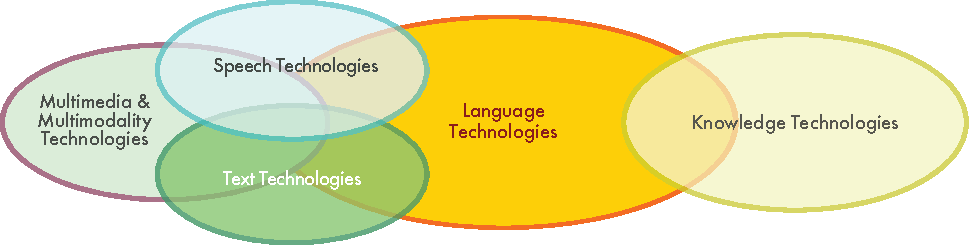
\includegraphics[width=\textwidth]{../_media/english/language_technologies}
  \caption{Language technology in context}
  \label{fig:ltincontext_en}
  \colorrule{grey3}{\textwidth}{1.5pt}
\end{figure*}

When we communicate, we combine language with other modes of communication and information media – for example speaking can involve gestures and facial expressions. Digital texts link to pictures and sounds. Movies may contain language in spoken and written form. In other words, speech and text technologies overlap and interact with other multimodal communication and multimedia technologies.\\ 
In this section, we will discuss the main application areas of language technology, i.\,e., language checking, web search, speech interaction, and machine translation. These applications and basic technologies include 

\begin{itemize}
\item spelling correction
\item authoring support
\item computer-assisted language learning
\item information retrieval 
\item information extraction
\item text summarisation
\item question answering
\item speech recognition 
\item speech synthesis 
\end{itemize}

Language technology is an established area of research with an extensive set of introductory literature. The interested reader is referred to the following references:  \cite{carstensen-etal1, jurafsky-martin01, manning-schuetze1, lt-world1, lt-survey1}.

Before discussing the above application areas, we will briefly describe the architecture of a typical LT system.

\subsection{Application Architectures}

Software applications for language processing typically consist of several components that mirror different aspects of language. While such applications are typically very complex, figure~\ref{fig:textprocessingarch_en} shows a highly simplified architecture of a typical text processing system. The first three modules handle the structure and meaning of the text input:

\begin{enumerate}
\item Pre-processing: cleans the data, analyses or removes formatting, detects the input languages, and so on.
\item Grammatical analysis: finds the verb, its objects, modifiers and other parts of speech; detects the sentence structure.
\item Semantic analysis: performs disambiguation (i.\,e., computes the appropriate meaning of words in a given context); resolves anaphora (i.\,e., which pronouns refer to which nouns in the sentence); represents the meaning of the sentence in a machine-readable way.
\end{enumerate}

After analysing the text, task-specific modules can perform other operations, such as automatic summarisation and database look-ups.

In the remainder of this section, we firstly introduce the core application areas for language technology, and follow this with a brief overview of the state of LT research and education today, and a description of past and present research programmes. Finally, we present an expert estimate of core LT tools and resources for German in terms of various dimensions such as availability, maturity and quality. The general situation of LT for the Dutch language is summarised in a matrix (figure~\ref{fig:lrlttable_en}). Tools and resources that are boldfaced in the text can also be found in figure~\ref{fig:lrlttable_en} (p.~\pageref{fig:lrlttable_en}) at the end of this chapter. LT support for Dutch is also compared to other languages that are part of this series.

\begin{figure*}[htb]
  \colorrule{grey3}{\textwidth}{1.5pt}
  \center
  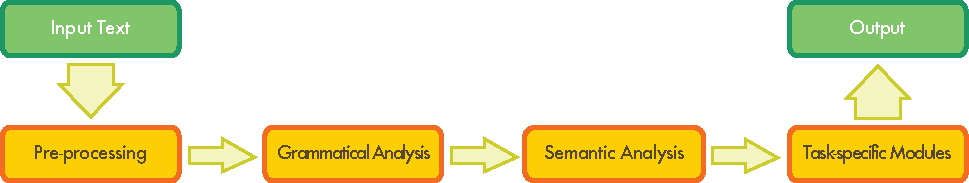
\includegraphics[width=\textwidth]{../_media/english/text_processing_app_architecture}
  \caption{A typical text processing architecture}
  \label{fig:textprocessingarch_en}
  \colorrule{grey3}{\textwidth}{1.5pt}
\end{figure*}

\subsection{Core Application Areas}

In this section, we focus on the most important LT tools and resources, and provide an overview of LT activities in Germany, Austria and Switzerland. 

\subsubsection{Language Checking}

Anyone who has used a word processor such as Microsoft Word knows that it has a spell checker that highlights spelling mistakes and proposes corrections. The first spelling correction programs compared a list of extracted words against a dictionary of correctly spelled words. Today these programs are far more sophisticated. Using language-dependent algorithms for \textbf{grammatical analysis}, they detect errors related to morphology (e.\,g., plural formation) as well as syntax–related errors, such as a missing verb or a conflict of verb-subject agreement (e.\,g., \textit{she *write a letter}). However, most spell checkers will not find any errors in the following text \cite{zar1}:

\begin{quote}
  I have a spelling checker,\\
  It came with my PC.\\
  It plane lee marks four my revue\\
  Miss steaks aye can knot sea.
\end{quote}

    For handling this type of errors, analysis of the context is needed in many cases, e.g., for deciding whether a verb has to be written with \emph{dt} or \emph{d} at the end in Dutch, as in:\\
\begin{itemize}
  \item  Hij heeft het dier \underline{verwond}.
 \item   (He has injured the animal)
 \item   Hij \underline{verwondt} het dier.
  \item  (He injures the animal.)
\end{itemize}


 This either requires the formulation of language-specific grammar rules, i.e. a high degree of expertise and manual labour, or the use of a so-called statistical language model.  Such models calculate the probability of a particular word occurring in a specific environment (i.e., the preceding and following words). For example, \emph{hij verwondt} is a much more probable word sequence than \emph{hij verwond}. A statistical language model can be automatically derived using a large amount of (correct) language data (i.e. a corpus). Up to now, these approaches have mostly been developed and evaluated on English language data. However, they do not necessarily transfer straightforwardly to Dutch with its more flexible word order, verb particle combinations, compounds, and crossing dependencies.

\begin{figure*}[htb]
  \colorrule{grey3}{\textwidth}{1.5pt}
  \center
  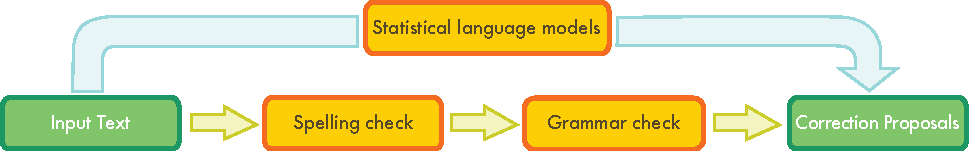
\includegraphics[width=\textwidth]{../_media/english/language_checking}
  \caption{Language checking (statistical; rule-based)}
  \label{fig:langcheckingaarch_en}
  \colorrule{grey3}{\textwidth}{1.5pt}
\end{figure*}

Language checking is not limited to word processors; it is also used in “authoring support systems”, i.\,e., software environments in which manuals and other types of technical documentation for complex IT, healthcare, engineering and other products, are written. To offset customer complaints about incorrect use and damage claims resulting from poorly understood instructions, companies are increasingly focusing on the quality of technical documentation while targeting the international market (via translation or localisation) at the same time. Advances in natural language processing have led to the development of authoring support software, which helps the writer of technical documentation to use vocabulary and sentence structures that are consistent with industry rules and (corporate) terminology restrictions.

\boxtext{The use of language checking is not limited to word processors. It also applies to authoring support systems.}

Proofing tools for Dutch that were incorporated in Microsoft products were developed in the past by Lernout \& Hauspie, independently later by Polderland, and this software is currently maintained and further developed by Knowledge Concepts.  Other companies active in this area are *TAL{\=O} BV and Carp technologies.

    Besides spell checkers and authoring support, Language Checking is also important in the field of computer-assisted language learning and is applied to automatically correct queries sent to Web Search engines, e.g. Google's `Did you mean\dots' suggestions.


\subsubsection{Web Search}

\begin{figure*}[htb]
  \colorrule{grey3}{\textwidth}{1.5pt}
  \center
  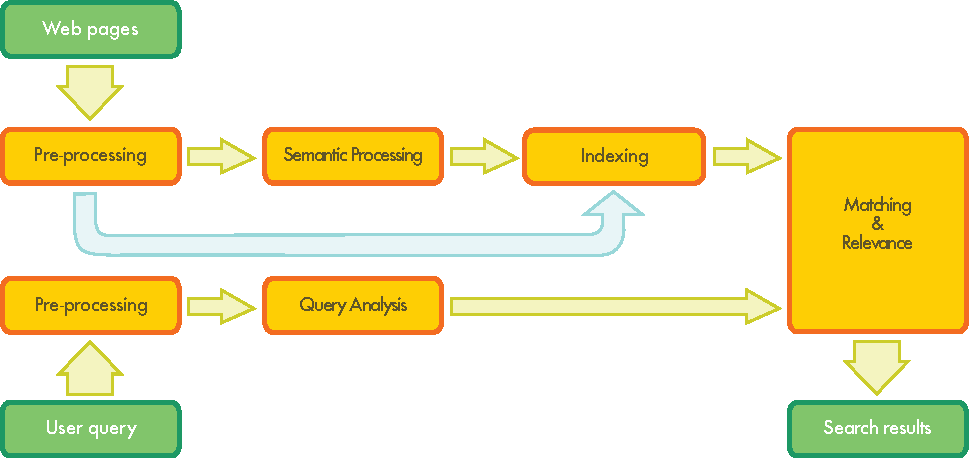
\includegraphics[width=\textwidth]{../_media/english/web_search_architecture}
  \caption{Web search}
  \label{fig:websearcharch_en}
  \colorrule{grey3}{\textwidth}{1.5pt}
 \end{figure*}

Searching the Web, intranets or digital libraries is probably the most widely used yet largely underdeveloped language technology application today. The search engine Google, which started in 1998, is nowadays used for about 80\% of all search queries world-wide \cite{Spiegel}. The verb \emph{googelen} even has an entry in the Dutch Van Dale dictionary. The Google search interface and results page display has not significantly changed since the first version. However, in the current version, Google offers spelling correction for misspelled words and incorporates basic semantic search capabilities that can improve search accuracy by analysing the meaning of terms in a search query context \cite{pc1}. The Google success story shows that a large volume of data and efficient indexing techniques can deliver satisfactory results using a statistical approach to language processing. 

For more sophisticated information requests, it is essential to integrate deeper linguistic knowledge to facilitate text interpretation. Experiments using \textbf{lexical resources} such as machine-readable thesauri or ontological language resources like WordNet (or the equivalent Dutch EuroWordNet) have demonstrated improvements in finding pages using synonyms of the original search terms, such as \textit{Atomkraft} {[}atomic energy{]}, \textit{Kernenergie} {[}atomic power{]} and \textit{Nuklearenergie} {[}nuclear energy{]}, or even more loosely related terms.

\boxtext{The next generation of search engines will have to include much more sophisticated language technology.}

The next generation of search engines will have to include much more sophisticated language technology, escpecially to deal with search queries consisting of a question or other sentence type rather than a list of keywords. For the query, \textit{Give me a list of all companies that were taken over by other companies in the last five years}, a syntactic as well as \textbf{semantic analysis} is required. The system also needs to provide an index to quickly retrieve relevant documents. A satisfactory answer will require syntactic parsing to analyse the grammatical structure of the sentence and determine that the user wants companies that have been acquired, rather than companies that have acquired other companies. For the expression \textit{last five years}, the system needs to determine the relevant range of years, taking into account the present year. The query then needs to be matched against a huge amount of unstructured data to find the pieces of information that are relevant to the user’s request. This process is called information retrieval, and involves searching and ranking relevant documents. To generate a list of companies, the system also needs to recognise a particular string of words in a document represents a company name, using a process called named entity recognition.

A more demanding challenge is matching a query in one language with documents in another language. Cross-lingual information retrieval involves automatically translating the query into all possible source languages and then translating the results back into the user's target language.

Now that data is increasingly found in non-textual formats, there is a need for services that deliver multimedia information retrieval by searching images, audio files and video data. In the case of audio and video files, a speech recognition module must convert the speech content into text (or into a phonetic representation) that can then be matched against a user query.

 In the Netherlands, several companies are active in these domains, including AskNow Solutions, Carp Technologies, GridLine, Irion Technologies, Knowledge Concepts, MediaLab Solutions, RightNow! (formerly Q-Go), TextKernel, and others. In Belgium Natlanco, InterSystems (formerly i.Know), ICMS, Aktor Technologies, Mentoring Systems and CrossMinder are active in these areas.

These companies focus their development on providing add-ons and advanced search engines for special interest portals by using topic-relevant semantics. Due to the constant high demand for processing power, such search engines are only cost-effective when handling relatively small text corpora. The processing time is several thousand times higher than that needed by a standard statistical search engine like Google. These search engines are in high demand for topic-specific domain modelling, but they cannot be used on the Web with its billions and billions of documents.



\subsubsection{Speech Interaction}

Speech interaction is one of many application areas that depend on speech technology, i.\,e., technologies for processing spoken language. Speech interaction technology is used to create interfaces that enable users to interact in spoken language instead of using a graphical display, keyboard and mouse.  Today, these voice user interfaces (VUI) are used for partially or fully automated telephone services provided by companies to customers, employees or partners. Business domains that rely heavily on VUIs include banking, supply chain, public transportation, and telecommunications. Other uses of speech interaction technology include interfaces to car navigation systems and the use of spoken language as an alternative to the graphical or touchscreen interfaces in smartphones.

\begin{figure*}[htb]
  \colorrule{grey3}{\textwidth}{1.5pt}
  \center
  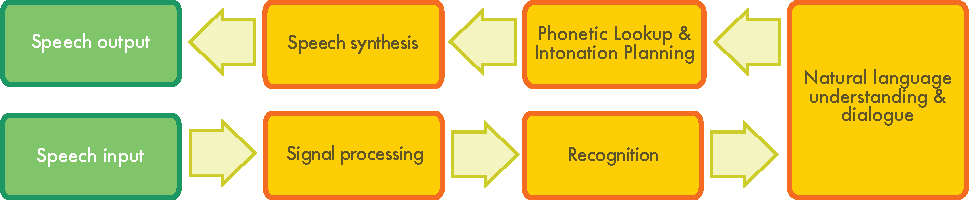
\includegraphics[width=\textwidth]{../_media/english/simple_speech-based_dialogue_architecture}
  \caption{Speech-based dialogue system}
  \label{fig:dialoguearch_en}
  \colorrule{grey3}{\textwidth}{1.5pt}
\end{figure*}

Speech interaction technology comprises four technologies: 

\begin{enumerate}
\item Automatic \textbf{speech recognition} (ASR) determines which words are actually spoken in a given sequence of sounds uttered by a user.  
\item Natural language understanding analyses the syntactic structure of a user’s utterance and interprets it according to the system in question.
\item Dialogue management determines which action to take given the user input and system functionality.   
\item \textbf{Speech synthesis} (text-to-speech or TTS) transforms the system’s reply into sounds for the user.
\end{enumerate}

One of the major challenges of ASR systems is to accurately recognise the words a user utters. This means restricting the range of possible user utterances to a limited set of keywords, or manually creating language models that cover a large range of natural language utterances. Using machine learning techniques, language models can also be generated automatically from \textbf{speech corpora}, i.\,e., large collections of speech audio files and text transcriptions. Restricting utterances usually forces people to use the voice user interface in a rigid way and can damage user acceptance; but the creation, tuning and maintenance of rich language models will significantly increase costs. VUIs that employ language models and initially allow a user to express their intent more flexibly — prompted by a \textit{How may I help you?} greeting — tend to be automated and are better accepted by users.

\boxtext{Speech interaction is the basis for creating interfaces that allow a user to interact with spoken language instead of a graphical dis-play, keyboard and mouse.}

Companies tend to use pre-recorded utterances by professional speakers for generating the output of the voice user interface. For static utterances where the wording does not depend on particular contexts of use or personal user data, this can deliver a rich user experience. But more dynamic content in an utterance may suffer from unnatural intonation because bits of audio files have simply been strung together. Through optimisation, today’s TTS systems are getting better at producing natural-sounding dynamic utterances.

Interfaces in speech interaction have been considerably standardised during the last decade in terms of their various technological components. There has also been strong market consolidation in speech recognition and speech synthesis. The national markets in the G20 countries (economically resilient countries with high populations) have been dominated by just five global players, with Nuance (USA) and Loquendo (Italy) being the most prominent players in Europe. In 2011, Nuance announced the acquisition of Loquendo, which represents a further step in market consolidation.

   On the Dutch TTS market, there are additional smaller companies like Acapela, based in Wallonia, SVOX, headquartered in Switzerland, and Fluency, based in Amsterdam. There are many companies that are active in using TTS and ASR technology in applications and services. These include Advance Voice Technology, DB-Scape, Dialogs Unlimited, DutchEar,   G2 Speech,  Logica, OrcaVoice, Quentris, Telecats, TomTom and Voice Data Bridge. Several companies and foundations focus on applications for user groups with specific demands such as physically handicapped people, dyslectic people, and elderly. These include Axendo, Cochlear Benelux, Dedicon, JABBLA, Kamelego, Lexima, rdgKompagne, Sensotec NV, and VoiceCore.

    Regarding dialogue management technology and know-how, some relevant companies are Carp technologies, Irion,  RightNow! (formerly Q-Go) and  RE-Phrase for text-based applications, and  Dialogs Unlimited, DutchEar, Telecats, and Voice Data Bridge for speech-based applications. Within the domain of speech interaction, a genuine market for the linguistic core technologies for syntactic and semantic analysis does not exist yet.

    As for the actual employment of VUIs, demand has increased within the last 5 years. This tendency has been driven by end customers' increasing demand for customer self-service and the considerable cost optimisation aspect of automated telephone services, as well as by a significantly increased acceptance of spoken language as a modality for man-machine interaction.

    Looking beyond today's state of technology, there will be significant changes due to the spread of smart phones as a new platform for managing customer relationships - in addition to the tele-phone, internet, and email channels. This tendency will also affect the employment of speech technology. On the one hand, demand for telephony-based VUIs will decrease, on the long run. On the other hand, the usage of spoken language as a user-friendly input modality for smart phones will gain significant importance. This tendency is supported by the observable improvement of speaker-independent speech recognition accuracy for speech dictation services that are already offered as centralised services to Smartphone users. Given this `outsourcing' of the recognition task to the infrastructure of applications, the application-specific employment of linguistic core technologies will supposedly gain importance compared to the present situation.

\subsubsection{Machine Translation}

\begin{figure*}[htb]
  \colorrule{grey3}{\textwidth}{1.5pt}
  \center
  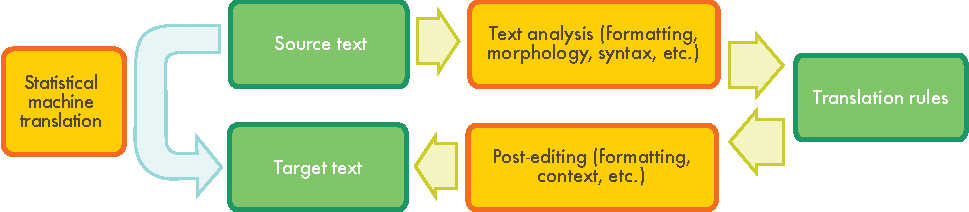
\includegraphics[width=\textwidth]{../_media/english/machine_translation}
  \caption{Machine translation (statistical; rule-based)}
  \label{fig:mtarch_en}
  \colorrule{grey3}{\textwidth}{1.5pt}
\end{figure*}

The idea of using digital computers to translate natural languages can be traced back to 1946 and was followed by substantial funding for research during the 1950s and again in the 1980s. 
Yet machine translation (MT) still cannot deliver on its initial promise of providing across-the-board automated translation.  

\boxtext{At its basic level, Machine Translation simply substitutes words in one natural language with words in another language.}

The most basic approach to machine translation is the automatic replacement of the words in a text written in one natural language with the equivalent words of another language. This can be useful in subject domains that have a very restricted, formulaic language such as weather reports.
However, in order to produce a good translation of less restricted texts, larger text units (phrases, sentences, or even whole passages) need to be matched to their closest counterparts in the target language. The major difficulty is that human language is ambiguous. Ambiguity creates challenges on multiple levels, such as word sense disambiguation on the lexical level (e.g. \emph{graven} can mean `counts',  `graves' or `to dig')  or the interpretation of relative pronouns (as subject or as object) on the syntactic level as in::

\begin{itemize}
\item De man die de vrouw zag.
\item (The man who saw the woman.) or (The man who the woman saw.)
\end{itemize}

One way to build an MT system is to use linguistic rules. For translations between closely related languages, a translation using direct substitution may be feasible in cases such as the above example. However, rule-based (or linguistic knowledge-driven) systems often analyse the input text and create an intermediary symbolic representation from which the target language text can be generated. The success of these methods is highly dependent on the availability of extensive lexicons with morphological, syntactic, and semantic information, and large sets of grammar rules carefully designed by skilled linguists. This is a very long and therefore costly process.

In the late 1980s when computational power increased and became cheaper, interest in statistical models for machine translation began to grow. Statistical models are derived from analysing bilingual text corpora, \textbf{parallel corpora}, such as the Europarl parallel corpus, which contains the proceedings of the European Parliament in 11 European languages. Given enough data, statistical MT works well enough to derive an approximate meaning of a foreign language text by processing parallel versions and finding plausible patterns of words. Unlike knowledge-driven systems, however, statistical (or data-driven) MT systems often generate ungrammatical output. Data-driven MT is advantageous because less human effort is required, and it can also cover special particularities of the language (e.\,g., idiomatic expressions) that are often ignored in knowledge-driven systems. 

The strengths and weaknesses of knowledge-driven and data-driven machine translation tend to be complementary, so that nowadays researchers focus on hybrid approaches that combine both methodologies. One such approach uses both knowledge-driven and data-driven systems, together with a selection module that decides on the best output for each sentence. However, results for sentences longer than, say, 12 words, will often be far from perfect. A more effective solution is to combine the best parts of each sentence from multiple outputs; this can be fairly complex, as corresponding parts of multiple alternatives are not always obvious and need to be aligned. 

\boxtext{Machine Translation is particularly challenging for the Dutch language.}

 For Dutch, MT is particularly challenging. The possibility of creating arbitrary new words by compounding makes dictionary analysis and dictionary coverage difficult; rather free word order, split verb constructions and R-pronouns pose problems for analysis.

    Leading commercial MT systems from the past like Systran, Globalink, LOGOS, METAL (and its spin-offs, LANT (currently Xplanation), GMS and Lucy Software), LMT developed by IBM (forming the basis for Linguatec  and Lingenio) never covered the Dutch language, probably because it was not interesting to do so from a commercial point of view. Only some research systems for Dutch were developed, partially in companies (Philips: Rosetta, BSO: Distributed Translation) and partially in academia (Utrecht University \& KU Leuven: Eurotra). Translation systems for Dutch were only produced when funded. For example, METAL produced a Dutch-French MT system for the ministries of Agriculture and Internal Affairs, and after the Dutch Language Union issued a call for the development of MT systems translating between Dutch on the one hand and English and French on the other in 1999 \cite{Cucchiarini:etal:2000},  funded by public money, Systran developed such systems in the context of the NL-Translex project.

    All systems mentioned above were knowledge-based. With the rise of statistical MT, Dutch has become a language quite generally covered. It is included in the 52 languages Google Translate offers and in the 24 languages SDL Language Weaver offers.

    The use of machine translation can significantly increase productivity provided the system is intelligently adapted to user-specific terminology and integrated into a workflow. Most MT companies stress that they can rapidly adapt their standard systems to com-pany-specific dictionaries, terminology and translation memories, thereby increasing MT quality significantly.

There is still a huge potential for improving the quality of MT systems. The challenges involve adapting language resources to a given subject domain or user area, and integrating the technology into workflows that already have term bases and translation memories. Another problem is that most of the current systems are English-centred and only support a few languages from and into Dutch. This leads to friction in the translation workflow and forces MT users to learn different lexicon coding tools for different systems.

Evaluation campaigns help to compare the quality of MT systems, the different approaches and the status of the systems for different language pairs. Figure~\ref{fig:euromatrix_de} (p.~\pageref{fig:euromatrix_de}), which was prepared during the EC Euromatrix+ project, shows the pair-wise performances obtained for 22 of the 23 official EU languages (Irish was not compared). The results are ranked according to a BLEU score, which indicates higher scores for better translations \cite{bleu1}. A human translator would normally achieve a score of around 80 points.

The best results (in green and blue) were achieved by languages that benefit from a considerable research effort in coordinated programmes and the existence of many parallel corpora (e.\,g., English, French, Dutch, Spanish and German). The languages with poorer results are shown in red. These languages either lack such development efforts or are structurally very different from other languages (e.\,g., Hungarian, Maltese and Finnish).

\subsection{Language Technology `behind the scenes'}

Building language technology applications involves a range of subtasks that do not always surface at the level of interaction with the user, but they provide significant service functionalities “behind the scenes” of the system in question. They all form important research issues that have now evolved into individual sub-disciplines of computational linguistics.  Question answering, for example, is an active area of research for which annotated corpora have been built and scientific competitions have been initiated. The concept of question answering goes beyond keyword-based searches (in which the search engine responds by delivering a collection of potentially relevant documents) and enables users to ask a concrete question to which the system provides a single answer. For example:

\textit{Question: How old was Neil Armstrong when he stepped on the moon?}\\
\textit{Answer: 38.}

While question answering is obviously related to the core area of web search, it is nowadays an umbrella term for such research issues as which different types of questions exist, and how they should be handled; how a set of documents that potentially contain the answer can be analysed and compared (do they provide conflicting answers?); and how specific information (the answer) can be reliably extracted from a document without ignoring the context. 

\boxtext{Language technology applications often provide significant service functionalities "behind the scenes” of larger software systems.}

Question answering is in turn related to information extraction (IE), an area that was extremely popular and influential when computational linguistics took a statistical turn in the early 1990s. IE aims to identify specific pieces of information in specific classes of documents, such as the key players in company takeovers as reported in newspaper stories. Another common scenario that has been studied is reports on terrorist incidents. The task here consists of mapping appropriate parts of the text to a template that specifies the perpetrator, target, time, location and results of the incident. Domain-specific template-filling is the central characteristic of IE, which makes it another example of a “behind the scenes” technology that forms a well-demarcated research area, which in practice needs to be embedded into a suitable application environment. 

    Text summarisation and \textbf{text generation} are two borderline areas that can act either as standalone applications or play a supporting role. Summarisation attempts to give the essentials of a long text in a short form, and is one of the features available in Microsoft Word. It mostly uses a statistical approach to identify the “important” words in a text (i.\,e., words that occur very frequently in the text in question but less frequently in general language use) and determine which sentences contain the most of these “important” words. These sentences are then extracted and put together to create the summary. In this very common commercial scenario, summarisation is simply a form of sentence extraction, and the text is reduced to a subset of its sentences. An alternative approach, for which some research has been carried out, is to generate brand new sentences that do not exist in the source text. 

\boxtext{For the Dutch language, research in most text technologies is much less developed than for the English language.}

For Dutch, the situation in all these research areas is much less developed than it is for English, where question answering, information extraction, and summarisation have since the 1990s been the subject of numerous open competitions, primarily those organised by DARPA/NIST in the United States. These have significantly improved the state of the art, but the focus has always been on English; some competitions have added multilingual tracks, but Dutch was never prominent, though some challenges are organised from Flanders \cite{SemEval}.  Nevertheless, work on question answering was promoted by the IMIX programme that focused on Interactive Multimodal Information eXtraction applied to Dutch resources \cite{IMIX}.  In this programme, question answering systems, with speech input and output, supporting follow-up questions were developed for the general domain and one specific for the medical domain. In addition, systems to generate textual output in combination with other modalities, and dialogue managers to connect all these systems were developed. The company RightNow (formerly Q-GO) from the Netherlands has been very successful in the area of textual question answer systems operating via chats or e-mail.  Eindhoven University (IPO) has worked on a language and speech generation system, that has later been acquired by Polderland (and probably now resides with Knowledge Concepts), but it appears hardly to have been used outside its original purpose \cite{Theune:2003}.  Tilburg University has worked on multi-document summarisation (integrating different messages on the same topic) in the STEVIN DAESO project \cite{DAESO}.  Nevertheless, there are hardly any annotated corpora or other resources for these tasks.

\subsection{LT Research and Education}

    In academia there are a number of excellent centres in the area of human language technology, e.g.  KU Leuven, Ghent university, Radboud University Nijmegen and University of Twente for speech technology, Tilburg and Antwerp universities for machine learning techniques in NLP, Utrecht University, and Leuven for NLP and machine translation, Groningen and Amsterdam for parsing, Amsterdam for sentiment mining and parsing, etc. It is, however, very difficult to attract students for the NLP field. Possible causes for this may be the relative low visibility of NLP in the university curricula and the fact that many NLP research groups are in the humanities (students there do not easily take a technical view on language, as is required for NLP).

    The academic players in the Netherlands and Flanders do not necessarily focus on the Dutch language: in research the focus is typically on English in order to be able to make sensible comparisons with researchers abroad. Nevertheless, several researchers are active in the area of Computer Aided Language Learning (CALL), where language and speech technology is used to increase language skills of first and second language learners. Relevant organisations include RU Nijmegen, University of Antwerp Linguapolis and KULAK.

  \subsection{Language Technology Industry}

 The LT field in the Netherlands and Belgium consist of many organisations, both industry (some 65) and knowledge centres (44) \cite{Orgs}.  The sector is reasonably well organised, with an active professional organisation NOTaS \cite{NOTAS} in the Netherlands consisting of 15 industrial and academic partners, the Flemish research community cooperating in CLIF \cite{CLIF}, and intense cooperation in the last decade between players from the Netherlands and Flanders, and from industry and academia in the joint Netherlands-Flanders LT programmes CGN (Spoken Dutch Corpus) \cite{CGN} and especially STEVIN \cite{STEVIN}. The SMEs in Flanders, however, are acting individually, and have not organised themselves in a sector, which makes them relatively invisible.

    Most industrial players are very small SMEs and have to struggle every day to survive, or they are small departments in a company that has a different focus for its core business activities. Nevertheless, some SMEs are quite successful and have been able to build up a stable business. Most SMEs in the area of speech technology are system integrators, application developers, or service providers. The actual development of technology, at least in speech technology, has been concentrated in a very few number of players (e.g. Nuance).

    One problem for marketing LT is that LT is not clearly visible because it is hidden as an integrated part of a more encompassing product or service, even though it is a component of products and services used by many users (e.g. search on the internet, texting on mobile phones, etc.).

    Even though there are many players in the Netherlands and Flanders, this does not imply that their focus is also on the Dutch language. For industry, the Dutch language is commercially less interesting than other languages, and the necessary investments can often not be justified by the small Dutch-language market.
    
\subsection{Language Technology Programs}

  Activities for the Dutch language have to be promoted and supported explicitly. Fortunately, this has been done in several programmes and projects over the last one and a half decade. Thus a Dutch language spoken train information system was developed as a carrier for research in speech analysis and generation, in language analysis and generation, and in dialogue management in the OVIS programme in the late nineties. The NL-Translex project was already mentioned above. Flanders had a short term programme on LT in the mid nineties. The IMIX programme, mentioned above, carried out research using systems for the Dutch language.  In the IOP MMI (Innovation Research Programme on Man Machine Interaction) and CATCH \cite{CATCH} programs language and speech technology have been used as tools for man machine interfaces and disclosing cultural heritage. Most prominent in their focus on the Dutch language are the joint Netherlands-Flanders CGN and STEVIN programmes. These have yielded significant progress in the availability of basic resources (data and tools) for the Dutch language, some initial research and several end user applications. Though some of the results achieved in these projects can be exploited in industry and in academia (e.g. in the CLARIN-NL research infrastructure \cite{CLARIN-NL} ) the prospects for optimally exploiting these results in actual research and in industry further are grim, since it appears not to have the focus of attention of the government in the Netherlands, and research has been reorganised so that it has become more difficult to get funding for discipline-specific programmes. The situation is probably a bit more positive in Flanders, though. Furthermore, some prerequisites for exploiting the potential are in place, such as visibility and accessibility of the resources produced in earlier programmes via the TST-Centrale (Dutch HLT Agency).

  The programmes mentioned also contributed significantly to bringing together the speech and language technology communities, which until recently were heterogeneous communities and operated quite separated from each other. These disciplines are distributed over computer or engineering science faculties (speech technology in Flanders, and in Twente; some language technology) and the humanities faculties (most though not all language technology) and generally meet in several separate conferences. The only exception may be the LREC conference \cite{LREC}, which however has a specific focus on language resources and evaluation.

  It is generally expected that the role of LT is going to be boosted enormously by the increasing growth of content that is ubiquitously available via an increasing amount of small mobile devices with large computational power (smart phones, iPad, etc.) and continuous access to the internet. Such devices have a relatively small screen, and no or primitive keyboards, which makes the use of speech increasingly more natural and necessary, and the amount of information they must search, summarise, translate or otherwise process requires an enormous boost in LT technology.

  It is therefore of the utmost importance that the activities started with the CGN and STEVIN programmes are continued, so that the scientific and commercial opportunities lying around the corner are optimally taken advantage of and the Dutch language and their native speakers can play a lasting role in the modern information and communication society also at the European level.

As we have seen, previous programmes have led to the development of a number of LT tools and resources for the Dutch language. The following section summarises the current state of LT support for Dutch.
  
\subsection{Availability of Tools and Resources}

Figure~\ref{fig:lrlttable_en} provides a rating for language technology support for the Dutch language. This rating of existing tools and resources was generated by leading experts in the field who provided estimates based on a scale from 0 (very low) to 6 (very high) using seven criteria.

\begin{figure*}[htb]
\centering
%\begin{tabular}{>{\columncolor{orange1}}p{.33\linewidth}ccccccc} % ORIGINAL
\begin{tabular}{>{\columncolor{orange1}}p{.33\linewidth}@{\hspace*{6mm}}c@{\hspace*{6mm}}c@{\hspace*{6mm}}c@{\hspace*{6mm}}c@{\hspace*{6mm}}c@{\hspace*{6mm}}c@{\hspace*{6mm}}c}
\rowcolor{orange1}
 \cellcolor{white}&\begin{sideways}\makecell[l]{Quantity}\end{sideways}
&\begin{sideways}\makecell[l]{\makecell[l]{Availability} }\end{sideways} &\begin{sideways}\makecell[l]{Quality}\end{sideways}
&\begin{sideways}\makecell[l]{Coverage}\end{sideways} &\begin{sideways}\makecell[l]{Maturity}\end{sideways} &\begin{sideways}\makecell[l]{Sustainability}\end{sideways} &\begin{sideways}\makecell[l]{Adaptability}\end{sideways} \\ \addlinespace
\multicolumn{8}{>{\columncolor{orange2}}l}{Language Technology: Tools, Technologies and Applications} \\ \addlinespace
 Speech Recognition&2,4&4,8&4,8&3,6&4,8&4,8&2,4\\ \addlinespace
Speech Synthesis&2,4&2,4&4,8&4,8&4,8&3,6&1,2\\ \addlinespace
Grammatical Analysis&3,6&5,4&4,8&3,6&4,8&3,6&1,8\\ \addlinespace
Semantic Analysis&0,8&4&3&3&2,4&1,6&1,6\\ \addlinespace
Text Generation&1,2&2,4&3,6&3&2,4&2,4&2,4\\ \addlinespace
Machine Translation&6&6&2,4&4,8&3,6&1,2&2,4\\ \addlinespace
  \multicolumn{8}{>{\columncolor{orange2}}l}{Sprachressourcen: Ressourcen, Daten und Wissensbanken} \\\addlinespace
Text corpora&2,4&6&4,8&2,4&4,2&4,8&2,4\\ \addlinespace
Speech corpora&2,4&4,8&6&4,8&4,8&4,8&1,2\\ \addlinespace
Parallel corpora&1,2&6&3,6&2,4&4,8&2,4&1,2\\ \addlinespace
Lexical resources&3&4,8&4,2&3,7&4,2&4,8&1,2\\ \addlinespace
Grammars&1,2&4,8&3,6&2,5&4,8&2,4&1,2\\ \addlinespace
\end{tabular}
\caption{State of language technology support for German}
\label{fig:lrlttable_en}
\end{figure*}

The key results for Dutch language technology can be summed up as follows:

\begin{itemize}
 \item Speech processing currently seems to be more mature than processing of written text (though more complex applications still pose serious challenges to speech technology).
 \item Advanced information access technologies are in their infancies (Information Extraction, Question Answering, Advanced Discourse Processing, Summarisation, etc.).
 \item The more linguistic and semantic knowledge a tool takes into account, the more gaps exist (see, e.g., information retrieval v. text semantics); more efforts for supporting deep linguistic processing are needed.
 \item	Research was successful in designing particular high quality software, but many of the resources lack standardisation and especially interoperability; concerted programs and initiatives are needed to make data and tools truly interoperable.
 \item	For Dutch, many resources created with public money in the recent LT programmes are either open source or stored, main-tained and distributed by the HLT Agency and easily and cheaply accessible. (cf. the high scores for Availability for Text Analysis, Text Interpretation, Text and Speech Corpora)
 \item 	Annotated corpora with semantic structures are available but minimal in size and depth of annotation. Annotated corpora with discourse structures are lacking almost completely, as are     Ontological resources for World Knowledge.
\item  	Parallel corpora for machine translation are available but in quantities that are too small for proper development of MT systems. MT, and especially statistical MT, needs huge amounts of (parallel) data to perform reasonably.
\item  	Multimedia data is a huge gap.
\end{itemize}

From this, it is clear that more efforts need to be directed into the creation of resources for Dutch and into research, innovation, and development. The need for large amounts of data and the high com-plexity of language technology systems make it also mandatory to develop new infrastructures for sharing and cooperation.

\subsection{Cross-language comparison}

The current state of LT support varies considerably from one language community to another. In order to compare the situation between languages, this section will present an evaluation based on two sample application areas (machine translation and speech processing) and one underlying technology (text analysis), as well as basic resources needed for building LT applications. The languages were categorised using the following five-point scale: 

\begin{enumerate}
\item Excellent support
\item Good support
\item Moderate support
\item Fragmentary support
\item Weak or no support
\end{enumerate}

LT support was measured according to the following criteria:

\textbf{Speech Processing:} Quality of existing speech recognition technologies, quality of existing speech synthesis technologies, coverage of domains, number and size of existing speech corpora, amount and variety of available speech-based applications.

\textbf{Machine Translation:} Quality of existing MT technologies, number of language pairs covered, coverage of linguistic phenomena and domains, quality and size of existing parallel corpora, amount and variety of available MT applications.

\textbf{Text Analysis:} Quality and coverage of existing text analysis technologies (morphology, syntax, semantics), coverage of linguistic phenomena and domains, amount and variety of available applications, quality and size of existing (annotated) text corpora, quality and coverage of existing lexical resources (e.\,g., WordNet) and grammars.

\textbf{Resources:} Quality and size of existing text corpora, speech corpora and parallel corpora, quality and coverage of existing lexical resources and grammars.

Figures~\ref{fig:speech_cluster_en} to~\ref{fig:resources_cluster_en} show that, thanks to large-scale LT funding in recent decades, the German language is better equipped than most other languages. It compares well with languages with a similar number of speakers, such as French, despite its greater structural complexity. But LT resources and tools for Dutch clearly do not yet reach the quality and coverage of comparable resources and tools for the English language, which is in the lead in almost all LT areas. And there are still plenty of gaps in English language resources with regard to high quality applications.

For speech processing, current technologies perform well enough to be successfully integrated into a number of industrial applications such as spoken dialogue and dictation systems. Today’s text analysis components and language resources already cover the linguistic phenomena of Dutch to a certain extent and form part of many applications involving mostly shallow natural language processing, e.\,g. spelling correction and authoring support.

However, for building more sophisticated applications, such as machine translation, there is a clear need for resources and technologies that cover a wider range of linguistic aspects and enable a deep semantic analysis of the input text. By improving the quality and coverage of these basic resources and technologies, we shall be able to open up new opportunities for tackling a broader range of advanced application areas, including high-quality machine translation.

\subsection{Conclusions}

\emph{In this series of white papers, we have made an important effort by assessing the language technology support for 30 European languages, and by providing a high-level comparison across these languages. By identifying the gaps, needs and deficits, the European language technology community and its related stakeholders are now in a position to design a large scale research and development programme aimed at building a truly multilingual, technology-enabled communication across Europe.}

The results of this white paper series show that there is a dramatic difference in language technology support for the various European languages. While there are good quality software and resources available for some languages and application areas, others, usually smaller languages, have substantial gaps. Many languages lack basic technologies for text analysis and the essential resources. Others have basic tools and resources but the implementation of for example semantic methods is still far away. Therefore a large-scale effort is needed to attain the ambitious goal of providing high-quality language technology support for all European languages, for example through high quality machine translation. 

   The situation of Dutch concerning language technology support gives rise to cautious optimism. Supported by larger research programs in the past, there exists a language technology industry and research scene in the Low Countries, which consists mostly of SMEs but is already partially organised.

    For standard Dutch, a number of technologies and resources exist, but far less than for English. As has been shown by several past studies on specific areas of language technology such as EuromatrixPlus, Dutch plays in Europe's second league together with German and French and few other languages. Still, this information has to be taken with care as even for English, language technology support today is by far not in a state that is needed for offering the support a true multilingual knowledge society needs.

    Our findings show that the Low Countries, after the successful CGN and STEVIN programmes should persist, and continue the development of language technology resources and use them to drive forward research, innovation and development. The need for large amounts of data and the extreme complexity of language technology systems makes it vital to develop a new infrastructure and a more coherent research organisation to spur greater sharing and cooperation.


Finally there is a lack of continuity in research and development funding. Short-term coordinated programmes tend to alternate with periods of sparse or zero funding. In addition, there is an overall lack of coordination with programmes in other EU countries and at the European Commission level.

The long term goal of META-NET is to enable the creation of high-quality language technology for all languages. This requires all stakeholders - in politics, research, business, and society - to unite their efforts. The resulting technology will help tear down existing barriers and build bridges between Europe’s languages, paving the way for political and economic unity through cultural diversity. 
\end{multicols}

\clearpage

\begin{figure*}[tb]
  \small
  \centering
  \begin{tabular}
  { % defines color for each column.
  >{\columncolor{corange5}}p{.13\linewidth}@{\hspace{.040\linewidth}}
  >{\columncolor{corange4}}p{.13\linewidth}@{\hspace{.040\linewidth}}
  >{\columncolor{corange3}}p{.13\linewidth}@{\hspace{.040\linewidth}}
  >{\columncolor{corange2}}p{.13\linewidth}@{\hspace{.040\linewidth}}
  >{\columncolor{corange1}}p{.13\linewidth} 
  }
  \multicolumn{1}{>{\columncolor{white}}c@{\hspace{.040\linewidth}}}{\textbf{Excellent}} & 
  \multicolumn{1}{@{}>{\columncolor{white}}c@{\hspace{.040\linewidth}}}{\textbf{Good}} &
  \multicolumn{1}{@{}>{\columncolor{white}}c@{\hspace{.040\linewidth}}}{\textbf{Moderate}} &
  \multicolumn{1}{@{}>{\columncolor{white}}c@{\hspace{.040\linewidth}}}{\textbf{Fragmentary}} &
  \multicolumn{1}{@{}>{\columncolor{white}}c}{\textbf{Weak/no}} \\ 
  \multicolumn{1}{>{\columncolor{white}}c@{\hspace{.040\linewidth}}}{\textbf{support}} & 
  \multicolumn{1}{@{}>{\columncolor{white}}c@{\hspace{.040\linewidth}}}{\textbf{support}} &
  \multicolumn{1}{@{}>{\columncolor{white}}c@{\hspace{.040\linewidth}}}{\textbf{support}} &
  \multicolumn{1}{@{}>{\columncolor{white}}c@{\hspace{.040\linewidth}}}{\textbf{support}} &
  \multicolumn{1}{@{}>{\columncolor{white}}c}{\textbf{support}} \\ \addlinespace
  
& \vspace*{0.5mm}English
& \vspace*{0.5mm}
Czech \newline 
Dutch \newline 
Finnish \newline 
French \newline 
German \newline   
Italian \newline  
Portuguese \newline 
Spanish \newline
& \vspace*{0.5mm}Basque \newline 
Bulgarian \newline 
Catalan \newline 
Danish \newline 
Estonian \newline 
Galician\newline 
Greek \newline  
Hungarian  \newline
Irish \newline  
Norwegian \newline 
Polish \newline 
Serbian \newline 
Slovak \newline 
Slovene \newline 
Swedish \newline
& \vspace*{0.5mm}
Croatian \newline 
Icelandic \newline  
Latvian \newline 
Lithuanian \newline 
Maltese \newline 
Romanian\\
\end{tabular}
\caption{Speech processing: state of language technology support for 30 European languages}
\label{fig:speech_cluster_en}
\end{figure*}

\begin{figure*}[tb]
  \small
  \centering
  \begin{tabular}
  { % defines color for each column.
  >{\columncolor{corange5}}p{.13\linewidth}@{\hspace{.040\linewidth}}
  >{\columncolor{corange4}}p{.13\linewidth}@{\hspace{.040\linewidth}}
  >{\columncolor{corange3}}p{.13\linewidth}@{\hspace{.040\linewidth}}
  >{\columncolor{corange2}}p{.13\linewidth}@{\hspace{.040\linewidth}}
  >{\columncolor{corange1}}p{.13\linewidth} 
  }
  \multicolumn{1}{>{\columncolor{white}}c@{\hspace{.040\linewidth}}}{\textbf{Excellent}} & 
  \multicolumn{1}{@{}>{\columncolor{white}}c@{\hspace{.040\linewidth}}}{\textbf{Good}} &
  \multicolumn{1}{@{}>{\columncolor{white}}c@{\hspace{.040\linewidth}}}{\textbf{Moderate}} &
  \multicolumn{1}{@{}>{\columncolor{white}}c@{\hspace{.040\linewidth}}}{\textbf{Fragmentary}} &
  \multicolumn{1}{@{}>{\columncolor{white}}c}{\textbf{Weak/no}} \\ 
  \multicolumn{1}{>{\columncolor{white}}c@{\hspace{.040\linewidth}}}{\textbf{support}} & 
  \multicolumn{1}{@{}>{\columncolor{white}}c@{\hspace{.040\linewidth}}}{\textbf{support}} &
  \multicolumn{1}{@{}>{\columncolor{white}}c@{\hspace{.040\linewidth}}}{\textbf{support}} &
  \multicolumn{1}{@{}>{\columncolor{white}}c@{\hspace{.040\linewidth}}}{\textbf{support}} &
  \multicolumn{1}{@{}>{\columncolor{white}}c}{\textbf{support}} \\ \addlinespace
  
& \vspace*{0.5mm} English 
& \vspace*{0.5mm} 
French \newline 
Spanish
& \vspace*{0.5mm}
Catalan \newline 
Dutch \newline 
German \newline 
Hungarian \newline
Italian \newline 
Polish \newline 
Romanian \newline 
& \vspace*{0.5mm}Basque \newline 
Bulgarian \newline 
Croatian \newline 
Czech \newline
Danish \newline 
Estonian \newline 
Finnish \newline 
Galician \newline 
Greek \newline 
Icelandic \newline 
Irish \newline 
Latvian \newline 
Lithuanian \newline 
Maltese \newline 
Norwegian \newline 
Portuguese \newline 
Serbian \newline 
Slovak \newline 
Slovene \newline 
Swedish \newline 
\end{tabular}
\caption{Machine translation: state of language technology support for 30 European languages}
\label{fig:mt_cluster_en}
\end{figure*}

\begin{figure*}[tb]
  \small
  \centering
  \begin{tabular}
  { % defines color for each column.
  >{\columncolor{corange5}}p{.13\linewidth}@{\hspace{.040\linewidth}}
  >{\columncolor{corange4}}p{.13\linewidth}@{\hspace{.040\linewidth}}
  >{\columncolor{corange3}}p{.13\linewidth}@{\hspace{.040\linewidth}}
  >{\columncolor{corange2}}p{.13\linewidth}@{\hspace{.040\linewidth}}
  >{\columncolor{corange1}}p{.13\linewidth} 
  }
  \multicolumn{1}{>{\columncolor{white}}c@{\hspace{.040\linewidth}}}{\textbf{Excellent}} & 
  \multicolumn{1}{@{}>{\columncolor{white}}c@{\hspace{.040\linewidth}}}{\textbf{Good}} &
  \multicolumn{1}{@{}>{\columncolor{white}}c@{\hspace{.040\linewidth}}}{\textbf{Moderate}} &
  \multicolumn{1}{@{}>{\columncolor{white}}c@{\hspace{.040\linewidth}}}{\textbf{Fragmentary}} &
  \multicolumn{1}{@{}>{\columncolor{white}}c}{\textbf{Weak/no}} \\ 
  \multicolumn{1}{>{\columncolor{white}}c@{\hspace{.040\linewidth}}}{\textbf{support}} & 
  \multicolumn{1}{@{}>{\columncolor{white}}c@{\hspace{.040\linewidth}}}{\textbf{support}} &
  \multicolumn{1}{@{}>{\columncolor{white}}c@{\hspace{.040\linewidth}}}{\textbf{support}} &
  \multicolumn{1}{@{}>{\columncolor{white}}c@{\hspace{.040\linewidth}}}{\textbf{support}} &
  \multicolumn{1}{@{}>{\columncolor{white}}c}{\textbf{support}} \\ \addlinespace

& \vspace*{0.5mm}English
& \vspace*{0.5mm}
  Dutch \newline 
  French \newline 
  German \newline 
  Italian \newline 
  Spanish
& \vspace*{0.5mm}Basque \newline 
  Bulgarian \newline 
  Catalan \newline 
  Czech \newline 
  Danish \newline 
  Finnish \newline 
  Galician \newline 
  Greek \newline 
  Hungarian \newline 
  Norwegian \newline 
  Polish \newline 
  Portuguese \newline 
  Romanian \newline 
  Slovak \newline 
  Slovene \newline 
  Swedish \newline 
& \vspace*{0.5mm}
  Croatian \newline 
  Estonian \newline 
  Icelandic \newline 
  Irish \newline 
  Latvian \newline 
  Lithuanian \newline 
  Maltese \newline 
  Serbian \\
  \end{tabular}
\caption{Text analysis: state of language technology support for 30 European languages}
\label{fig:text_cluster_en}
\end{figure*}

\begin{figure*}[tb]
  \small
  \centering
  \begin{tabular}
  { % defines color for each column.
  >{\columncolor{corange5}}p{.13\linewidth}@{\hspace{.040\linewidth}}
  >{\columncolor{corange4}}p{.13\linewidth}@{\hspace{.040\linewidth}}
  >{\columncolor{corange3}}p{.13\linewidth}@{\hspace{.040\linewidth}}
  >{\columncolor{corange2}}p{.13\linewidth}@{\hspace{.040\linewidth}}
  >{\columncolor{corange1}}p{.13\linewidth} 
  }
  \multicolumn{1}{>{\columncolor{white}}c@{\hspace{.040\linewidth}}}{\textbf{Excellent}} & 
  \multicolumn{1}{@{}>{\columncolor{white}}c@{\hspace{.040\linewidth}}}{\textbf{Good}} &
  \multicolumn{1}{@{}>{\columncolor{white}}c@{\hspace{.040\linewidth}}}{\textbf{Moderate}} &
  \multicolumn{1}{@{}>{\columncolor{white}}c@{\hspace{.040\linewidth}}}{\textbf{Fragmentary}} &
  \multicolumn{1}{@{}>{\columncolor{white}}c}{\textbf{Weak/no}} \\ 
  \multicolumn{1}{>{\columncolor{white}}c@{\hspace{.040\linewidth}}}{\textbf{support}} & 
  \multicolumn{1}{@{}>{\columncolor{white}}c@{\hspace{.040\linewidth}}}{\textbf{support}} &
  \multicolumn{1}{@{}>{\columncolor{white}}c@{\hspace{.040\linewidth}}}{\textbf{support}} &
  \multicolumn{1}{@{}>{\columncolor{white}}c@{\hspace{.040\linewidth}}}{\textbf{support}} &
  \multicolumn{1}{@{}>{\columncolor{white}}c}{\textbf{support}} \\ \addlinespace
    
& \vspace*{0.5mm}English
& \vspace*{0.5mm} 
    Czech \newline 
    Dutch \newline 
    French \newline 
    German \newline 
    Hungarian \newline
    Italian \newline
    Polish \newline
    Spanish \newline
    Swedish \newline 
& \vspace*{0.5mm} Basque\newline 
    Bulgarian\newline 
    Catalan \newline 
    Croatian \newline 
    Danish \newline 
    Estonian \newline 
    Finnish \newline 
    Galician \newline 
    Greek \newline 
    Norwegian \newline 
    Portuguese \newline 
    Romanian \newline 
    Serbian \newline 
    Slovak \newline 
    Slovene \newline
&  \vspace*{0.5mm}
    Icelandic \newline 
    Irish \newline 
    Latvian \newline 
    Lithuanian \newline 
    Maltese  \\
  \end{tabular}
  \caption{Speech and text resources: State of support for 30 European languages}  
  \label{fig:resources_cluster_en}
\end{figure*}

\cleardoublepage

% --------------------------------------------------------------------------
\ssection[About META-NET]{About META-NET}

\begin{multicols}{2}
META-NET is a Network of Excellence funded by the European Commission. The network currently consists of 54 members from 33 European countries \cite{rehm2011}. META-NET fosters the Multilingual Europe Technology Alliance (META), a growing community of language technology professionals and organisations in Europe. META-NET cooperates with other initiatives like the Common Language Resources and Technology Infrastructure (CLARIN), which is helping establish digital humanities research in Europe. META-NET fosters the technological foundations for a truly multilingual European information society that:

\begin{itemize}
\item makes communication and cooperation possible across languages;
\item provides equal access to information and knowledge in any language;
\item offers advanced and affordable networked information technology to European citizens.
\end{itemize}

META-NET stimulates and promotes multilingual technologies for all European languages. The technologies enable automatic translation, content production, information processing and knowledge management for a wide variety of applications and subject domains. The network wants to improve current approaches, so better communication and cooperation across languages can take place. Europeans have an equal right to information and knowledge regardless of language.

META-NET launched on 1 February 2010 with the goal of advancing research in language technology (LT). The network supports a Europe that unites as a single digital market and information space. META-NET has conducted several activities that further its goals. META-VISION, META-SHARE and META-RESEARCH are the network’s three lines of action.

\textbf{META-VISION} fosters a dynamic and influential stakeholder community that unites around a shared vision and a common strategic research agenda (SRA). The main focus of this activity is to build a coherent and cohesive LT community in Europe by bringing together representatives from highly fragmented and diverse groups of stakeholders. In the first year of META-NET, presentations at the FLaReNet Forum (Spain), Language Technology Days (Luxembourg), JIAMCATT 2010 (Luxembourg), LREC 2010 (Malta), EAMT 2010 (France) and ICT 2010 (Belgium) centred on public outreach. According to initial estimates, META-NET has already contacted more than 2,500 LT professionals to develop its goals and visions with them. At the META-FORUM 2010 event in Brussels, META-NET communicated the initial results of its vision building process to more than 250 participants. In a series of interactive sessions, the participants provided feedback on the visions presented by the network. 

\textbf{META-SHARE} creates an open, distributed facility for exchanging and sharing resources. The peer-to-peer network of repositories will contain language data, tools and web services that are documented with high-quality metadata and organised in standardised categories. The resources can be readily accessed and uniformly searched. The available resources include free, open source materials as well as restricted, commercially available, fee-based items. META-SHARE targets existing language data, tools and systems as well as new and emerging products that are required for building and evaluating new technologies, products and services. The reuse, combination, repurposing and re-engineering of language data and tools plays a crucial role. META-SHARE will eventually become a critical part of the LT marketplace for developers, localisation experts, researchers, translators and language professionals from small, mid-sized and large enterprises. META-SHARE addresses the full development cycle of LT—from research to innovative products and services. A key aspect of this activity is establishing META-SHARE as an important and valuable part of a European and global infrastructure for the LT community. 

\textbf{META-RESEARCH} builds bridges to related technology fields. This activity seeks to leverage advances in other fields and to capitalise on innovative research that can benefit language technology. In particular, this activity wants to bring more semantics into machine translation (MT), optimise the division of labour in hybrid MT, exploit context when computing automatic translations and prepare an empirical base for MT. META-RESEARCH is working with other fields and disciplines, such as machine learning and the Semantic Web community. META-RESEARCH focuses on collecting data, preparing data sets and organising language resources for evaluation purposes; compiling inventories of tools and methods; and organising workshops and training events for members of the community. This activity has already clearly identified aspects of MT where semantics can impact current best practices. In addition, the activity has created recommendations on how to approach the problem of integrating semantic information in MT. META-RESEARCH is also finalising a new language resource for MT, the Annotated Hybrid Sample MT Corpus, which provides data for English-German, English-Spanish and English-Czech language pairs. META-RESEARCH has also developed software that collects multilingual corpora that are hidden on the Web.
\end{multicols}

\vfill
\centerline{office@meta-net.eu -- http://www.meta-net.eu}

\cleardoublepage

\appendix
\addtocontents{toc}{\protect\bigskip}

\bsection[Literaturverweise --- References]{XXXLiteraturverweise --- References}
\bibliographystyle{unsrt} % What is the difference between "unsrt" und "is-unsrt"?
%\bibliographystyle{is-unsrt}
\bibliography{dutch}
  
\cleardoublepage

\bsection[META-NET Leden -- META-NET Members]{META-NET Leden --- META-NET Members}
\label{metanetmembers}

\small

\begin{longtable}{@{}llp{113mm}@{}}
  Belgien & \textcolor{grey1}{Belgium} & Computational Linguistics and Psycholinguistics Research Centre, University of Antwerp: Walter Daelemans\\ \addlinespace
  & & Centre for Processing Speech and Images, University of Leuven: Dirk van Compernolle \\ \addlinespace
  Bulgarien & \textcolor{grey1}{Bulgaria} & Institute for Bulgarian Language, Bulgarian Academy of Sciences: Svetla Koeva \\ \addlinespace
  Deutschland & \textcolor{grey1}{Germany} & Language Technology Lab, DFKI: Hans Uszkoreit, Georg Rehm\\ \addlinespace
  & & Human Language Technology and Pattern Recognition, RWTH Aachen University: Hermann Ney \\ \addlinespace
  & & Department of Computational Linguistics, Saarland University: Manfred Pinkal\\ \addlinespace Dänemark &  \textcolor{grey1}{Denmark} & Centre for Language Technology, University of Copenhagen: \newline Bolette Sandford Pedersen, Bente Maegaard\\ \addlinespace
  Estland & \textcolor{grey1}{Estonia} & Institute of Computer Science, University of Tartu: Tiit Roosmaa, Kadri Vider\\ \addlinespace
  Finnland & \textcolor{grey1}{Finland} & Computational Cognitive Systems Research Group, Aalto University: Timo Honkela\\ \addlinespace
  & & Department of Modern Languages, University of Helsinki: Kimmo Koskenniemi, Krister Lindén \\ \addlinespace
  Frankreich & \textcolor{grey1}{France} & Centre National de la Recherche Scientifique, Laboratoire d'Informatique pour la Mécanique et les Sciences de l'Ingénieur: Joseph Mariani \\ \addlinespace
  & & Evaluations and Language Resources Distribution Agency: Khalid Choukri\\ \addlinespace 
  Griechenland & \textcolor{grey1}{Greece} & R.C. “Athena”, Institute for Language and Speech Processing: Stelios Piperidis\\ \addlinespace
  Großbritannien & \textcolor{grey1}{UK} & 
  School of Computer Science, University of Manchester: Sophia Ananiadou \\ \addlinespace 
  & & Institute for Language, Cognition and Computation, Center for Speech Technology Research, University of Edinburgh: Steve Renals \\ \addlinespace 
  & & Research Institute of Informatics and Language Processing, University of Wolverhampton: Ruslan Mitkov \\ \addlinespace 
  Irland & \textcolor{grey1}{Ireland} & School of Computing, Dublin City University: Josef van Genabith\\ \addlinespace
  Island & \textcolor{grey1}{Iceland} & School of Humanities, University of Iceland: Eiríkur Rögnvaldsson\\ \addlinespace
  Italien & \textcolor{grey1}{Italy} & Consiglio Nazionale delle Ricerche, Istituto di Linguistica Computazionale “Antonio Zampolli”: Nicoletta Calzolari\\ \addlinespace
  & & Human Language Technology Research Unit, Fondazione Bruno Kessler:\newline Bernardo Magnini\\ \addlinespace 
  Kroatien & \textcolor{grey1}{Croatia} & Institute of Linguistics, Faculty of Humanities and Social Science, University of Zagreb: Marko Tadić \\ \addlinespace
  Lettland & \textcolor{grey1}{Latvia} & Tilde: Andrejs Vasiļjevs\\ \addlinespace 
  & & Institute of Mathematics and Computer Science, University of Latvia: Inguna Skadiņa\\ \addlinespace
  Litauen & \textcolor{grey1}{Lithuania} & Institute of the Lithuanian Language: Jolanta Zabarskaitė\\ \addlinespace
  Luxemburg & \textcolor{grey1}{Luxembourg} & Arax Ltd.: Vartkes Goetcherian\\ \addlinespace
  Malta & \textcolor{grey1}{Malta} & Department Intelligent Computer Systems, University of Malta: Mike Rosner\\ \addlinespace
  Niederlande & \textcolor{grey1}{Netherlands} & Utrecht Institute of Linguistics, Utrecht University: Jan Odijk\\ \addlinespace 
  & & Computational Linguistics, University of Groningen: Gertjan van Noord\\ \addlinespace
  Norwegen & \textcolor{grey1}{Norway} & Department of Linguistic, University of Bergen: Koenraad De Smedt\\ \addlinespace 
  & & Department of Informatics, Language Technology Group, University of Oslo:\newline Stephan Oepen \\ \addlinespace
  Österreich & \textcolor{grey1}{Austria} & Zentrum für Translationswissenschaft, Universität Wien: Gerhard Budin\\ \addlinespace 
  Polen & \textcolor{grey1}{Poland} & Institute of Computer Science, Polish Academy of Sciences: Adam Przepiórkowski, Maciej Ogrodniczuk \\ \addlinespace
  & & University of Łódź: Barbara Lewandowska-Tomaszczyk, Piotr Pęzik\\ \addlinespace
  & & Department of Computer Linguistics and Artificial Intelligence, Adam Mickiewicz University: Zygmunt Vetulani \\ \addlinespace
  Portugal & \textcolor{grey1}{Portugal} & University of Lisbon: António Branco, Amália Mendes \\ \addlinespace
  & & Spoken Language Systems Laboratory, Institute for Systems Engineering and Computers: Isabel Trancoso \\ \addlinespace
  Rumänien & \textcolor{grey1}{Romania} & Research Institute for Artificial Intelligence, Romanian Academy of Sciences:\newline Dan Tufiș \\ \addlinespace
  & & Faculty of Computer Science, University Alexandru Ioan Cuza of Iași: Dan Cristea \\ \addlinespace
  Schweden & \textcolor{grey1}{Sweden} & Department of Swedish, University of Gothenburg: Lars Borin \\ \addlinespace 
  Schweiz & \textcolor{grey1}{Switzerland} & Idiap Research Institute: Hervé Bourlard \\ \addlinespace 
  Serbien & \textcolor{grey1}{Serbia} & University of Belgrade, Faculty of Mathematics: Duško Vitas, Cvetana Krstev,\newline Ivan Obradović \\ \addlinespace
  & & Pupin Institute: Sanja Vranes \\ \addlinespace  
  Slowakei & \textcolor{grey1}{Slovakia} & Ľudovít Štúr Institute of Linguistics, Slovak Academy of Sciences: Radovan Garabík \\ \addlinespace 
  Slowenien & \textcolor{grey1}{Slovenia} & Jozef Stefan Institute: Marko Grobelnik \\ \addlinespace 
  Spanien & \textcolor{grey1}{Spain} & Barcelona Media: Toni Badia, Maite Melero \\ \addlinespace 
  & & Institut Universitari de Lingüística Aplicada, Universitat Pompeu Fabra: Núria Bel \\ \addlinespace 
  & & Aholab Signal Processing Laboratory, University of the Basque Country:\newline Inma Hernaez Rioja \\ \addlinespace 
  & & Center for Language and Speech Technologies and Applications, Universitat Politècnica de Catalunya:  Asunción Moreno \\ \addlinespace 
  & & Department of Signal Processing and Communications, University of Vigo:\newline Carmen García Mateo \\ \addlinespace 
  Tschechien & \textcolor{grey1}{Czech Republic} & Institute of Formal and Applied Linguistics, Charles University in Prague: Jan Hajič \\ \addlinespace
  Ungarn & \textcolor{grey1}{Hungary} & Research Institute for Linguistics, Hungarian Academy of Sciences: Tamás Váradi\\  \addlinespace
  & & Department of Telecommunications and Media Informatics, Budapest University of Technology and Economics: Géza Németh and Gábor Olaszy\\ \addlinespace
  Zypern & \textcolor{grey1}{Cyprus} & Language Centre, School of Humanities: Jack Burston
\end{longtable}
\normalsize

\renewcommand*{\figureformat}{}
\renewcommand*{\captionformat}{}

\begin{figure*}[htbp]
  \colorrule{grey3}{\textwidth}{1.5pt}
  \center
  %\fbox{-- META-NET group picture omitted to keep the size of the PDF file small. --}
  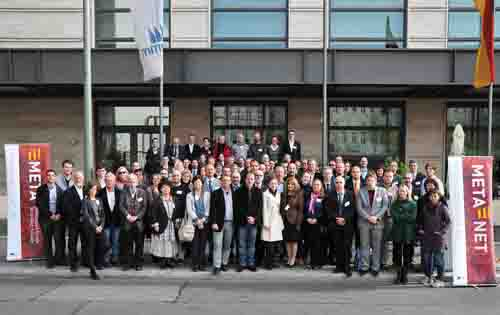
\includegraphics[width=\textwidth]{../_media/meta-net_team.jpg}
  \caption{Etwa 100 Experten des Gebiets Sprachtechnologie -- Repräsentanten der in META-NET vertretenen Länder und Sprachen -- diskutierten und finalisierten die zentralen Ergebnisse der Weißbuch-Serie bei einem META-NET-Treffen in Berlin am 21./22.~Oktober 2011. --- \textcolor{grey1}{About 100 language technology experts -- representatives of the countries and languages represented in META-NET -- discussed and finalised the key results and messages of the White Paper Series at a META-NET meeting in Berlin, Germany, on October 21/22, 2011.}}
  \medskip
  \colorrule{grey3}{\textwidth}{1.5pt}
\end{figure*}

\cleardoublepage

\bsection[Die META-NET Weissbuch-Serie -- The META-NET White Paper Series]{Die META-NET Weissbuch-Serie --- The META-NET\ \ \ \ \ \ White Paper Series}
\label{whitepaperseries}

\vspace*{-5mm}
\centering
  \setlength{\tabcolsep}{2em}
  \begin{tabularx}{\textwidth}{lllll} \toprule\addlinespace
  %\begin{tabulary}{170mm}{LLL} \toprule
  &Baskisch & Basque & euskara& \\
  &Bulgarisch & Bulgarian & български& \\
  &Dänisch & Danish & dansk& \\
  &Deutsch & German & Deutsch& \\
  &Englisch & English & English& \\
  &Estnisch & Estonian & eesti& \\
  &Finnisch & Finnish & suomi& \\
  &Französisch & French & français& \\
  &Galizisch & Galician & galego& \\
  &Griechisch & Greek & ελληνικά& \\
  &Isländisch & Icelandic & íslenska& \\
  &Irisch & Irish & Gaeilge& \\
  &Italienisch & Italian & italiano& \\
  &Katalanisch & Catalan & català& \\
  &Kroatisch & Croatian & hrvatski& \\
  &Lettisch & Latvian & latviešu valoda& \\
  &Litauisch & Lithuanian & lietuvių kalba& \\
  &Maltesisch & Maltese & Malti& \\
  &Niederländisch & Dutch & Nederlands& \\
  &Norwegisch Bokmål & Norwegian Bokmål & bokmål& \\
  &Norwegisch Nynorsk & Norwegian Nynorsk & nynorsk& \\
  &Polnisch & Polish & polski& \\
  &Portugiesisch & Portuguese & português& \\
  &Rumänisch & Romanian & română& \\
  &Serbisch & Serbian & српски& \\
  &Slowakisch & Slovak & slovenčina& \\
  &Slowenisch & Slovene & slovenščina& \\
  &Spanisch & Spanish & español& \\
  &Schwedisch & Swedish & svenska& \\
  &Tschechisch & Czech & čeština& \\
  &Ungarisch & Hungarian & magyar& \\ \addlinespace \bottomrule
\end{tabularx}

\end{document}